%% Adaptado a partir de :
%% abtex2-modelo-trabalho-academico.tex, v-1.9.2 laurocesar
%% para ser um modelo para os trabalhos no IFSP-SPO

\documentclass[
    % -- opções da classe memoir --
    12pt,               % tamanho da fonte
    openright,          % capítulos começam em pág ímpar (insere página vazia caso preciso)
    %twoside,            % para impressão em verso e anverso. Oposto a oneside
    oneside,
    a4paper,            % tamanho do papel6. 
    % -- opções da classe abntex2 --schwinn
    % Opções que não devem ser utilizadas na versão final do documento
    % draft,              % para compilar mais rápido, remover na versão final
    paginasA4,  % indica que vai utilizar paginas em A4 
    %MODELO,             % indica que é um documento modelo então precisa dos geradores de texto
    %TODO,               % indica que deve apresentar lista de pendencias 
    % -- opções do pacote babel --
    english,            % idioma adicional para hifenização
    brazil              % o último idioma é o principal do documento
    ]{ifsp-spo-inf-cemi} % ajustar de acordo com o modelo desejado para o curso

% ---
% Pacotes básicos 
% ---
\usepackage[utf8]{inputenc}     % Codificacao do documento (conversão automática dos acentos)
% ---

%\usepackage{style}
        

% --- 
% CONFIGURAÇÕES DE PACOTES ADICIONAIS UTEIS
% --- 


% ---
% Informações de dados para CAPA e FOLHA DE ROSTO
% ---
\titulo{IFriends: uma comunidade virtual}

% Trabalho individual
%\autor{AUTOR DO TRABALHO}

% Trabalho em Equipe
% ver também https://github.com/abntex/abntex2/wiki/FAQ#como-adicionar-mais-de-um-autor-ao-meu-projeto
\renewcommand{\imprimirautor}{
\begin{tabular}{lr}
ANAÍ VILLCA ROJAS & SP3029085 \\
JAMILLI VITÓRIA GIOIELLI & SP3027473 \\
JOSÉ ROBERTO CLAUDINO FERREIRA & SP3024369 \\
JULIA ROMUALDO PEREIRA & SP3023061 \\
KAIKY MATSUMOTO SILVA & SP185075X \\
\end{tabular}
}


\disciplina{PDS - Prática de Desenvolvimento de Sistemas}

\preambulo{Projeto de sistema IFriends apresentado, conforme as normas ABNT, à disciplina de Prática para Desenvolvimento de Sistemas.}

\data{2022}

% Definir o que for necessário e comentar o que não for necessário
% Utilizar o Nome Completo, abntex tem orientador e coorientador
% então vão ser utilizados na definição de professor
\renewcommand{\orientadorname }{Professor:}
\coorientador{Carlos Henrique Verissimo Pereira}
\renewcommand{\coorientadorname}{Professor:}
\orientador{Johnata Souza Santicioli}


% ---


% informações do PDF
\makeatletter
\hypersetup{
        %pagebackref=true,
        pdftitle={\@title}, 
        pdfauthor={\@author},
        pdfsubject={\imprimirpreambulo},
        pdfcreator={LaTeX with abnTeX2 using IFSP model},
        pdfkeywords={abnt}{latex}{abntex}{abntex2}{IFSP}{\ifspprefixo}{trabalho acadêmico}, 
        colorlinks=true,            % false: boxed links; true: colored links
        linkcolor=blue,             % color of internal links
        citecolor=blue,             % color of links to bibliography
        filecolor=magenta,              % color of file links
        urlcolor=blue,
        bookmarksdepth=4
}
\makeatother
% --- 


% ----
% Início do documento
% ----
\begin{document}


% Retira espaço extra obsoleto entre as frases.
\frenchspacing 

%somente para o exemplo, fica primeiro
%\newcommand{\urlmodelosimples}{https://www.overleaf.com/project/58a3a66af9bb74023ba1bd56}

\newcommand{\urlmodelo}{\url{\urlmodelosimples}}

Esse documento foi feito a partir do modelo canônico do \abnTeX, o acesso ao PDF pode ser feito em 
\urlmodelo. A estrutura utilizada aqui foi um modelo utilizado no curso de Pós Graduação em Gestão de TI do \ac{ifsp}.
\todo[inline]{Remover texto informativo inicial}


Este documento não pode ser considerado como um padrão a ser seguido em sua totalidade, ele tem como maior objetivo demonstrar como utilizar o \LaTeX\ para obter um documento atendendo ao máximo o padrão do \ac{ifsp} e \ac{abnt}.

Faça leitura dos arquivos fonte \LaTeX\ e não somente do PDF gerado.

Esse documento é, em princípio, uma cópia do utilizado na disciplina de PDS e irá sofrer alterações durante o ano letivo. Essas alterações buscam induzir os alunos à prática com o \LaTeX\ . 

Algumas bibliotecas \LaTeX\ disponíveis no overleaf estão desatualizadas, para melhores resultados é recomendável a utilização de outro compilador utilizando as ultimas versões de todas bibliotecas.

Leia com cuidado :
\begin{itemize}
    \item \url{https://dicas.ivanfm.com/aulas/textos/};
    \item \url{https://dicas.ivanfm.com/aulas/textos/revisao-de-textos.html};
    \item exemplos no \autoref{cap-exemplos};
    \item \autoref{elementos-nao-textuais} sobre elementos não textuais que fala sobre o maior problema dos alunos que é de tentar posicionar as ilustrações.
\end{itemize}


\noindent\hrulefill


% -- lista de pendencias gerada pelo todonotes
% -- altere opções do usepackage para remover na versão final....
% \textit{\listoftodos
% \todo[inline]{remover lista de todo da versão final...}
% \newpage}

% ----------------------------------------------------------
% ELEMENTOS PRÉ-TEXTUAIS
% ----------------------------------------------------------
\pretextual

% ---
% Capa
% ---
\imprimircapa

\newcounter{todocounter}
\newcommand{\todonum}[2][]
{\stepcounter{todocounter}\todo[#1]{\thetodocounter: #2}}


% ---

% ---
% Folha de rosto
% (o * indica que haverá a ficha bibliográfica)
% ---
\imprimirfolhaderosto
%\imprimirfolhaderosto*
% ---

%Caso necessário
% ----------------------------------------------------------
%\input{pre/01-pre-errata}
% ----------------------------------------------------------

%Obrigatório para trabalhos com bancas oficiais
% ----------------------------------------------------------
%\input{pre/02-pre-aprovacao}
% ----------------------------------------------------------

% ---- opcionais 
% ----------------------------------------------------------
%\input{pre/03-pre-dedicatoria}
% ----------------------------------------------------------
% ---
% Agradecimentos
% ---
\begin{agradecimentos}

Os agradecimentos principais são direcionados a Deus e aos membros da equipe Bunka Bytes, que trabalharam juntos para desenvolver está aplicação, sempre unidos e ajudando uns aos outros. 

Agradecemos também aos nossos professores orientadores da disciplina de \acs{pds}, Johnata Souza Santicioli e Carlos Henrique Veríssimo Pereira, que pacientemente nos auxiliaram e nos ajudaram a construir o presente trabalho.

E por último, mas não menos importante, aos nossos amigos e familiares por nos apoiarem neste processo de desenvolvimento e nos incentivarem a seguir firmes e fortes. 

\end{agradecimentos}
% ---
% ----------------------------------------------------------
% ---
% Epígrafe
% ---
\begin{epigrafe}
    \vspace*{\fill}
    \begin{flushright}
        \textit{``Se quer ir rápido, vá sozinho. \\
                  Se quer ir longe, vá em grupo.'' \\
                  (Provérbio africano)}
    \end{flushright}
\end{epigrafe}
% ---




% ----------------------------------------------------------

% -- resumo obrigatório
% ----------------------------------------------------------
% ---
% RESUMOS
% ---

% resumo em português
\setlength{\absparsep}{18pt} % ajusta o espaçamento dos parágrafos do resumo
\begin{resumo}

O objetivo central deste trabalho é apresentar a projeção e a implementação de um produto mínimo viável em formato de sistema Web para a construção de uma comunidade virtual, em busca da criação de um espaço de acolhimento de alunos para alunos. Propõe-se, assim, utilizar de um método ágil e de ferramentas de desenvolvimento para passar pelos processos de engenharia do sistema, além de estimular o trabalho em equipe. Sob essa perspectiva, o projeto pôde ser apresentado abordando seu tema principal e focando nas suas funcionalidades mais essenciais, como as perguntas e respostas, o perfil do usuário e a gestão de eventos.


\textbf{Palavras-chaves}: Projeto. Comunidade virtual.
\end{resumo}

% resumo em inglês
\begin{resumo}[Abstract]
\begin{otherlanguage*}{english}

The main goal of this project is to present the design and implementation of a minimum valuable product in terms of a web software, for the construction of the virtual community and in order to create a supportive environment from students to students. Hence, the team intends to use an agile methodology and development tools to go through the software engineering process and encourage the team work. Under this perspective, the project could be presented focusing on its main goal and functionalities related to the minimum user needs, such as the questions and answers, the user profile and the event management.

  \vspace{\onelineskip}
  \noindent 
  \textbf{Keywords}: Project. Virtual Community.
 \end{otherlanguage*}
\end{resumo}
% ----------------------------------------------------------

% ---
% inserir lista de ilustrações
% ---
\pdfbookmark[0]{\listfigurename}{lof}
\listoffigures*
\cleardoublepage
% ---

% % ---
% % inserir lista de tabelas
% %---
% \pdfbookmark[0]{\listtablename}{lot}
% \listoftables*
% \cleardoublepage
% % ---

% ---
% inserir lista de quadros
% ---
\pdfbookmark[0]{\listofquadrosname}{loq}
\listofquadros*
\cleardoublepage
% ---

\input{pre/07-pre-siglas}
% ----------------------------------------------------------
%\input{pre/08-pre-simbolos}
% ----------------------------------------------------------

% ---
% inserir o sumario
% ---
\pdfbookmark[0]{\contentsname}{toc}
\tableofcontents*
\cleardoublepage
% ---


% ----------------------------------------------------------
% ELEMENTOS TEXTUAIS
% ----------------------------------------------------------
\textual


% ----------------------------------------------------------
% Introdução (exemplo de capítulo sem numeração, mas presente no Sumário)
% ----------------------------------------------------------
\chapter{Introdução}
O presente documento é resultado da proposta de um projeto cujo objetivo é sustentado no planejamento e na execução de um sistema para a Web através do aprendizado obtido nas matérias técnicas do Curso Técnico de Informática, realizado no \acs{ifsp}, e como forma de trabalho de conclusão de curso.

Tendo isto em vista e diante dos desafios presentes na lista de requisitos e orientações propostas para a iniciação deste projeto, os integrantes da equipe Bunka Bytes reuniram-se em busca de encontrar a solução que melhor se encaixasse em seus objetivos e nos da disciplina de \acs{pds}.

Portanto, este documento apresenta o processo de desenvolvimento do \gls{ifriends}, desde a origem do projeto, até sua execução final, documentando o acompanhamento de todas as atividades executadas pelos membros da equipe para sua elaboração. 

%-------------------------------------------------------------------------------
\section{Origem do Projeto}
% ------------------------------------------------------------------------------
E foi pensando em soluções viáveis que a equipe voltou seu olhar para sistemas que contribuem para a criação de comunidades colaborativas na área de desenvolvimento de sistemas, que, segundo \citeonline{rosa2008identidade}, foi fortemente difundida pelas comunidades de Código Aberto (do inglês, \textsl{Open Source}), sendo primeiramente criada pela cultura \textsl{hacker}, na qual afirma que a paixão e o interesse dos \textsl{hackers} nas soluções foi uma das principais propulsoras do espírito colaborativo.

Além deles, foi trazido ao debate as possibilidades de aliar as principais dificuldades que os integrantes observaram durante sua vida acadêmica no \acs{ifsp}, a um sistema que pudesse suprir determinadas necessidades dos alunos, como os questionamentos que começam a surgir com mais frequência conforme o início dos estudos é dado, sendo eles em âmbitos diversos como: sobre a instituição de ensino, matérias e assuntos tratados no ensino médio, dúvidas sobre os conteúdos técnicos ou até mesmo a busca por um apoio educacional - como ocorrem nas monitoriais. 

O Instituto Federal de São Paulo (\acs{ifsp}), especificamente no campus São Paulo, cenário onde os integrantes da equipe estão inseridos e também público-alvo que a comunidade pretende atingir, é uma instituição de ensino que fornece ensino médio, técnicos profissionalizantes e graduações.
Por ser um ambiente novo e repleto de informações simultâneas, muitos alunos ingressantes ficam perdidos no momento de lidar com coisas cotidianas, como: funcionamento da instituição, quantidade de disciplinas, volume de atividades, novas pessoas para se conviver, liberdade e responsabilidade que é concedida ao aluno, entre muitas outras. Isso torna o \acs{ifsp} um ambiente muito desafiador que pode gerar inúmeras dúvidas entre os novos alunos. 

O \gls{ifriends} surge nesse cenário, no qual a criação de uma comunidade de estudantes que colaborassem entre si, pudesse instigar o interesse dos alunos em ajudarem uns aos outros de maneira acessível e prática, onde uma dúvida estivesse a um palmo de distância.

%-------------------------------------------------------------------------------
\section{Pesquisa de viabilidade} 
\label{pesquisa}
% ------------------------------------------------------------------------------
Foi realizada pela equipe uma pesquisa de viabilidade da aplicação, visando verificar se o público-alvo realmente estava sendo atingido, ou seja, se os alunos da instituição possuem interesse na aplicação e pretendem utilizar a mesma como ferramenta cotidiana para auxilia-los durante os estudos.

Para isto, houve a elaboração de um formulário por meio da ferramenta \gls{googleforms}, onde solicitamos que os alunos da instituição respondessem, com sinceridade, dez questões (\autoref{questões}) sobre a proposta. Sua divulgação ocorreu por meio do aplicativo de conversas \gls{WhatsApp}, onde os integrantes da equipe ficaram responsáveis por enviar o endereço de compartilhamento do formulário nos grupos de alunos conhecidos na instituição.

A realização desta pesquisa é de grande importância para a equipe avaliar a proposta que está sendo apresentada e para analisar sua viabilidade por meio dos resultados.

%-------------------------------------------------------------------------------
\subsection{Resultados}
%-------------------------------------------------------------------------------
A partir deste formulário, foram recebidas \textbf{quarenta e cinco} respostas acumuladas dentro de um período de \textbf{cinco} dias, e ao final, foi possível constatar as seguintes características na maioria das respostas:

Algumas características do maior grupo que responderam ao questionário são: 

\begin{itemize}
    \item 86,7\% dos estudantes são do ensino médio integrado ao técnico;
    \item 66,7\% dos que sentiram dificuldade ao ingressar no \glsxtrshort{ifsp}, compartilhou em forma de resposta curta suas experiências (como, adaptação com as atividades, dificuldades em matérias específicas, falta de transparência nas informações institucionais);
    \item 60\% nunca frequentaram ou vão raramente às monitorias;
    \item 85,5\% usariam o sistema e acreditam que o mesmo o ajudaria academicamente;
\end{itemize}

Com base nesses resultados, a equipe entende que a proposta cumpre seu proposito de atingir os alunos do \glsxtrshort{ifsp} com o desenvolvimento de uma comunidade de apoio aos assuntos enfrentados durante sua formação.

% ------------------------------------------------------------------------------
\section{Objetivo}
% ------------------------------------------------------------------------------
%Nesta seção serão descritos os respectivos objetivos (principal e específico) pretendidos com a iniciação deste projeto. 
%\subsection{Objetivo Principal}

Dadas as informações citadas anteriormente, o objetivo deste projeto é tentar instigar o interesse dos estudantes que compreendem o \acs{ifsp} para poderem criar espaços colaborativos, por um sistema no qual os usuários interajam entre perguntas e respostas, fornecendo caminhos para o esclarecimento de suas dúvidas sobre a instituição de ensino, as áreas e disciplinas que a ela pertence.  

Dessa forma, o objetivo será aplicado através da construção de uma plataforma de perguntas, respostas e mentorias para a Web, em que a comunidade interna poderá submeter uma pergunta para ser respondida pelos outros membros da comunidade; além de possibilitar que estudantes possam escolher se tornar mentores sobre determinados assuntos, disponibilizando recursos para a criação de anúncios de eventos de monitorias (cuja localidade a eles deve competir) dentro de seus perfis de usuário. 

Tendo isso em vista e pensando numa melhor interatividade entre os membros da comunidade, o sistema deve passar por um processo de \gls{gamificação} em algumas de suas funcionalidades, como as votações para respostas e perguntas mais relevantes e os atributos dos usuários mais ativos  - assim como outros exemplos que devem ser adicionados durante o planejamento do projeto.

%\subsection{Objetivos Específicos}
%Dado o objetivo principal do projeto, o objetivo específico descrito nesta seção dá-se em forma de proposta de implementação do sistema citado anteriormente, na qual descrevemos um resumo da aplicação e seus propósitos, tendo em vista sua importância social e suas especificações técnicas.

\section{Justificativa}
A reflexão com relação às formas complementares de aprendizagem é importante para a ampliação dos conteúdos interessados tanto aos alunos, quanto aos seus professores, pois permite que enxerguem, juntos, o ensino como um meio que evite a passagem de aprendizados de forma restrita e hierarquizada.

Por isso, \citeonline{fernandes2011redes} traz em sua pesquisa que o desafio da construção de sociedades de aprendizagem parte do pressuposto de que os recursos tecnológicos disponibilizados atualmente permitem aos estudantes aprenderem dentro e fora da escola e das mais variadas formas. Assim, para ele, a melhor forma se dá ``construindo comunidades sustentadas pelo uso de tecnologias Web''.

O autor dá continuidade na exposição desse fenômeno ao atribuir o sucesso da potencialização da aprendizagem complementar e das relações sociais à ``Web 2.0''. Isto, pois, de acordo \citeonline{fernandes2011redes}, a mesma permitiu novas formas e possibilidades de criação de conteúdos e possibilitou o enfoque a uma aprendizagem motivada pelos interesses do aluno, em que ele deve assumir um papel exploratório nessa experiência, da qual poderá colher ensinamentos significativos, explica \citeonline{fernandes2011redes}.

Visando atrair atenção para o tema, o projeto tem como principal missão, permitir que os estudantes possam usufruir de uma ferramenta gratuita que proporcione a suavização do seu processo de aprendizagem, quando seus próprios colegas contribuirão com suas experiências passadas, além de deixarem um histórico para possibilitar um caminho menos árduo aos estudantes que virão. Por isso, espera-se que, com este projeto, a instituição de ensino também seja um agente na construção de uma comunidade propícia para estudantes, onde poderão unir-se em razão de dúvidas comuns, e assim incentivarem a disseminação de uma cultura colaborativa dentro de seus espaços.

% dar mais profundidade?

\section{Análise de Concorrência}
Além disso, levou-se em consideração uma análise de concorrência com plataformas que apresentem características semelhantes ou até mesmo parecidas com as que gostaríamos de oferecer. Dessa forma, pretendemos demostrar melhor como o nosso projeto se destaca em relação à concorrência e no que ele pode agregar.

Como primeiro concorrente pensamos no \gls{moodle} já que ele faz parte da vida de muitos alunos do \acs{ifsp}, pois ele é usado como ferramenta complementar de estudos. Ele fornece, nas disciplinas criadas pelos professores, a possibilidade de criar um fórum e também dispõem uma versão mobile.

Como segundo concorrente pensou-se no \gls{scoold} devido a ser uma inspiração para o nosso projeto, já que o mesmo possui quase todas as funcionalidades pensadas para o \gls{ifriends}, mas seu foco é em fornecer um espaço de perguntas e respostas. 

Dessa forma, o \autoref{AnalisedeConcorrencia} apresenta a comparação dessas duas plataformas com o projeto de sistemas \gls{ifriends}:

\def\arraystretch{2}
\begin{quadro}[htb]
\centering
\ABNTEXfontereduzida
\caption{Análise de Concorrência}
\label{AnalisedeConcorrencia}
\resizebox{\linewidth}{!}{
\begin{tabular}{|p{8cm}|c|c|c|}
\hline
\thead{Funcionalidades} & \thead{IFriends} & \thead{Moodle} & \thead{Scoold} \\
\hline

Comunicação pública (fórum) entre as partes envolvidas & \circlemark &  & \circlemark \\ \hline
Publicação de eventos & \circlemark &  &  \\ \hline
Publicação de perguntas & \circlemark & \circlemark & \circlemark \\ \hline
Filtro de pesquisa no fórum de perguntas & \circlemark &  & \circlemark \\ \hline
Filtro de pesquisa nos eventos & \circlemark &  &  \\ \hline
Gamificação & \circlemark &  & \circlemark \\ \hline
Acesso à plataforma por aplicativo móvel &  & \circlemark &  \\ \hline

\end{tabular}}\legend{Fonte: Os autores}
\end{quadro}
\FloatBarrier

Devido ao curto tempo de desenvolvimento, uma questão que ficou em aberto, em relação às funcionalidades propostas no \autoref{AnalisedeConcorrencia} foi essa questão da versão \textit{mobile}. Mas isso não foi considerado uma questão muito prejudicial para o desenvolvimento do projeto, visto que, o que levou a tal escolha foi a priorização em desenvolver melhor as outras funcionalidades, visto que a nossa missão visa a criação de uma comunidade que facilite e quebre essa barreira de interação entre as partes envolvidas.

Além disso, boas práticas de programação serão tomadas na elaboração do projeto, logo, a versão \textit{mobile} poderá ser trabalhada futuramente sem muitos impedimentos.

% ----------------------------------------------------------
% -----------------------------------------------------------------------
\chapter{Revisão da Literatura}
% -----------------------------------------------------------------------
Os assuntos tratados nesta seção pretendem apresentar o que já é sabido na comunidade científica, a respeito do tema proposto para ser discutido durante a execução do presente projeto. 
% -----------------------------------------------------------------------
\section{Construção de comunidades e redes aprendizado virtuais}

A partir da discussão iniciada no estudo de \citeonline{sartori2004comunidades} sobre as redes virtuais de aprendizado, toma-se como base a definição da construção de comunidades em torno de tais características como manifestações dos agrupamentos humanos dentro do ciberespaço. \citeonline{sartori2004comunidades} dão continuidade na introdução ao assunto, quando explicam o funcionamento da construção inicial de comunidades virtuais:
\begin{citacao}

Seu funcionamento está diretamente ligado, num primeiro momento, às redes de conexões proporcionadas pelas tecnologias de informação e comunicação e, num segundo momento, à possibilidade de, neste espaço, pessoas com objetivos comuns, se encontrarem, estabelecerem relações, e desenvolverem novas subjetividades \cite{sartori2004comunidades}.

\end{citacao}

Neste contexto, percebe-se que as características determinantes em uma comunidade virtual giram em torno ``de um sentimento de pertencimento e de um projeto comum'' oriundo da comunicação entre os indivíduos inseridos dentro deste espaço. Por conseguinte, \citeonline{sartori2004comunidades} afirmam que os grupos formados dentro de tais comunidades possuem vínculos sociais que se originam dos fluxos informacionais e comunicacionais, além das atividades e discussões fomentadas nas interações sociais, dentro das quais as pessoas formam unidades a partir de seus interesses comuns. 

Sabendo disso, dentro de sua argumentação, as autoras compreendem o conceito de socialidade presente nas dimensões de comunidades virtuais como um fenômeno independente de regulações que deve ser viabilizado ``através de comunicação multi-direcional que permite que os indivíduos possam estar ligados coletivamente'', além de completarem dizendo que o sentimento de pertencimento nestes espaços só é possível devido a ações executadas a distância, visto que a participação das pessoas tece “uma rede de cooperação oportunizada pelo processo de comunicação bidirecional'', explicam \citeonline{sartori2004comunidades}.

Por fim, \citeonline{sartori2004comunidades} finalizam a introdução ao assunto concluindo que para potencializar novas práticas educativas, comunicacionais, culturais e formar socialidades que possibilitem o ``exercício da cidadania, do desenvolvimento da cultura e de novos saberes'' em comunidades virtuais de aprendizagem, é necessário compreender, de antemão, que:
\begin{citacao}

Para que as comunidades virtuais de aprendizagem oportunizem a sensação de pertencimento, do “estar junto”, torna-se necessário investigar quais as características que devem estar presentes para possibilitar novas experiências culturais, sociais e educativas. Aqui se encontra, sem dúvida, um programa de estudos, pesquisas e reflexões que aprofundem o papel de formação de socialidades destas comunidades, ultrapassando a compreensão de suas possibilidades técnicas e de suas práticas protocolares \cite{sartori2004comunidades}.

\end{citacao}

Dentro desde cenário, é possível tentar compreender algumas das formas de estímulo para que a socialidade característica das comunidades virtuais se manifeste. Desse modo, o autor \citeonline{kratochwill2006possibilidades} descreve como exemplo a utilização de fóruns de discussão como parte do processo.
Segundo \citeonline{kratochwill2006possibilidades}, entende-se por fórum de discussão com finalidades educacionais um determinado espaço de comunicação formado por mensagens, que podem ou não seguir um padrão de classificação. Neste espaço, os usuários podem realizar contribuições, assim como esclarecer e contrariar os demais envolvidos de forma assíncrona.

O desenvolvimento de fóruns \textit{online} surge como uma nova perspectiva de escrita colaborativa capaz de fornecer a interação, debates e favorecer na aprendizagem colaborativa, diz \citeonline{kratochwill2006possibilidades}. O autor ainda afirma que alguns possíveis motivos para abrir um fórum \textit{online} de discussão seriam: o estímulo do espírito de participação, o compartilhamento de experiências, dúvidas e conhecimentos.


Assim, ficam notórias as contribuições que os ambientes virtuais podem trazer, isto, pois, \citeonline{kratochwill2006possibilidades} afirma ser interessante o desenvolvimento da dinâmica quando comenta:

\begin{citacao}

Torna-se interessante a dinâmica desenvolvida no fórum on-line pela sua perspectiva dialógica. Todos os participantes têm a oportunidade de se expressar, interferir e receber interferências, se constituir a partir da constituição do outro e da percepção do outro sobre a expressão do primeiro. Dentro desse processo dialógico, a autonomia e a autoria se constituem em respeito à alteridade, à individualidade e, ao mesmo tempo, em que coletivamente \cite{kratochwill2006possibilidades}.

\end{citacao}

Por outro lado, seguindo a mesma linha de pensamento, outro instrumento para estimular tais características na construção de comunidades de aprendizagem, pode ser a troca de conhecimentos através de monitorias, conforme conta \citeonline{friedlander1984alunos} ao afirmar que as monitorias ``proporcionam ampla troca dos mais diversos conhecimentos entre as partes envolvidas: alunos, monitores e professores''. 
Conforme \citeonline{matoso2014importancia} conta em seu relato de experiência como monitor, a monitoria trouxera-lhe ganhos importantes inclusive em aspectos interpessoais, isto porque, devido à grande procura dos alunos à monitoria apenas no período de provas, muitos chegavam angustiados e tristes, exigindo-lhe uma postura mais séria e confiante para lidar com estes estudantes.

Portanto, a importância de ser um monitor, segundo \citeonline{lins2009importancia}, está principalmente relacionada ao fato de que a melhor forma de se aprender um conteúdo é transmitindo o conhecimento, e neste contexto, o fácil diálogo do monitor com os professores e alunos, o torna o principal receptor nesta rede de troca de conhecimentos. Com isso, é possível aproximar ainda mais os alunos de seu processo educacional, tendo em vista que a troca de conhecimentos e experiências pode ser feita entre os próprios estudantes - praticando assim a socialidade, conforme demonstrado nos argumentos de \citeonline{sartori2004comunidades}.

% -----------------------------------------------------------------------
\section{Interatividade e propostas de gamificação}
Dando continuidade na reflexão acerca de métodos de aprimoramento da experiência de aprendizagem, a gamificação se coloca como um instrumento poderoso para a criação de espaços que sejam mediados por expressões de desafios e entretenimento, conforme contam \citeonline{valentim2016interatividade} em seu artigo, onde consideram a gamificação como aliada “na direção de novas formas de ensinar e aprender, e no cenário educativo online, alia-se à perspectiva da interatividade, novas possibilidades para a prática educativa” \cite{valentim2016interatividade}.

Ainda que este campo de estudo seja relativamente novo na literatura, as autoras argumentam que, dentro do contexto da Sociedade Digital, a interatividade é potencializada pelo uso de estratégias de gamificação, que envolve “uma diversidade de tecnologias no ambiente virtual, com a multiplicidade de interfaces existente”, tendo em vista que com ela é possível criar atividades diferenciadas que motivem a participação do estudante no espaço de aprendizagem. Com isso, \citeonline{valentim2016interatividade} completam que:

\begin{citacao}

[…] A interatividade se consolida como através da possibilidade de o indivíduo intervir na mensagem (Participação-Intervenção), de colaboração e coautoria, onde não existe fronteiras entre emissão e recepção (Bidirecionalidade-Hibridação) e por fim concretiza novas possibilidades de combinar informações produzir narrativas, múltiplas redes de conexões (Potencialidade-Permutabilidade). Interatividade é mais interação, participação, trocas, autoria, coautoria, cooperação, permite o compartilhamento, enfim, aprender através do diálogo e pelas múltiplas interfaces, construir aprendizagem colaborativa […] \cite{valentim2016interatividade}.

\end{citacao}
Seguindo uma linha de raciocínio similar, \citeonline{costa2018revisao} conta que a gamificação tem como objetivo motivar os usuários no processo de aprendizagem e participação na ferramenta na qual é utilizada essa metodologia, ela possui diversos elementos e também possíveis subcomponentes que, juntos, auxiliam para o seu propósito, sendo eles: exploração, cooperação, \textit{feedback}, antecipação, inovação, conquistas, sistema de recompensas, cultura de motivação e social. 

Os autores ressaltam ainda que esses elementos não compõem obrigatoriamente a gamificação, porém, quanto maior a presença deles, mais eficaz torna-se sua ferramenta. Além disso, não existem elementos mais importantes que outros, afirmam \citeonline{costa2018revisao}. Porém, dentre os elementos descritos por \citeonline{costa2018revisao}, o  \textit{feedback}  se destaca em sua característica motivacional, visto que pode estimular o usuário a realizar determinada ação quando aliado a subcomponentes como:

\begin{citacao}

Ao acertar, errar ou conquistar algo dentro de um sistema gamificado, o usuário deve obter uma resposta rápida e precisa, ou \textit{feedback} instantâneo. Ao utilizar algo simbólico como forma de responder ao usuário, o sistema acaba com isso, aumentando ou diminuindo a motivação dele para determinada ação, pois ao ver que o sistema responde algo quando se acerta ou erra, o usuário se sente encorajado a continuar ou não a atividade proposta. São elementos que incorporam o aspecto de \textit{feedback} da gamificação \cite{costa2018revisao}.

\end{citacao}

Além disso, o artigo conta que associados a estes elementos estão os emblemas, crachás ou distintivos (também conhecidos como \textsl{badges}, que trazem uma característica mais próxima a jogos quando aliados ao uso de pontuação (acúmulo de pontos que pode ser numérico ou simbólico), sendo estes elementos possíveis de serem utilizados juntos como um sistema de níveis a serem acrescidos para o usuário, descrevem \citeonline{costa2018revisao} e completa  \citeonline{zichermann2011gamification}.

Dessa forma, de acordo com \citeonline{orrico2012mercado}, um dos motivos para a utilização da gamificação como proposta de usabilidade, se dá pela grande base de pessoas que jogam ao redor do mundo, muitos se sentem mais motivados e dão retornos positivos quando existem elementos de jogos, os quais já são algo do cotidiano de grande parcela da população. Porém, é possível concluir que, ainda que a gamificação traga diversos benefícios, é preciso partir de determinados pressupostos para que seja aplicada de maneira adequada a somar com a interatividade no processo educativo. 

Isto, pois, conforme contam \citeonline{valentim2016interatividade}, enquanto a interatividade ``é mais participação, mais trocas, autoria, colaboração, coautoria, é um mais comunicacional'', a gamificação urge como aparelho de inovação no processo de educação digital para concretizar atividades colaborativas diferenciadas, conforme completa ao descrever:

\begin{citacao}
Cruzadinhas,  produção de  podcast,  videocast,  desafios  surpresas  aliados  a  interfaces  de colaboração do  AVA  como  chat,  fórum  de  discussão,  portfólio e  elementos  dos  games  como ranking,  desafios,  colaboração,  competição, pode  possibilitar  com  que  haja  motivação  pelos discentes, engajamento no processo educativo, e assim compreendemos a gamificação como elemento que pode favorecer a concretização da interatividade \cite{valentim2016interatividade}.
\end{citacao}


% -----------------------------------------------------------------------
% ----------------------------------------------------------
% ------------------------------------------------------------
\chapter{Materiais e Métodos}
% ------------------------------------------------------------
Segundo \citeonline{Junior:2010}, engenharia de \textsl{software} é ``um conjunto integrado de métodos e ferramentas utilizadas para especificar, projetar, implementar e manter um sistema'', e que, para tanto, reúne em si metodologias, métodos e ferramentas para que o projeto seja bem definido em todas as suas etapas, variando desde sua problemática inicial e indo até sua entrega enquanto um produto de \textsl{software}. É a partir disto, que \citeonline{Junior:2010} distingue um método de uma ferramenta:

\begin{citacao}
Um método é uma prescrição explícita de como chegar a uma atividade requerida por um modelo de ciclo de vida, visando otimizar a execução das atividades que foram especificadas. Já as ferramentas proporcionam apoio automatizado ou semi-automatizado aos métodos \cite{Junior:2010}.
\end{citacao}

Ademais, \citeonline{Junior:2010} ainda separa os métodos de desenvolvimento de sistema em três categoriais que permitem visualizar e solucionar o problema de diferentes maneiras para sua modelagem. Para a composição do presente projeto, no entanto, será utilizado como método principal a metodologia escolhida para a gestão do projeto e as ferramentas poderão ou não ser relacionadas a mesma, como há de ser especificado nas próximas seções.

%-------------------------------------------------------------
\section{Ferramentas de desenvolvimento}
%-------------------------------------------------------------
Pensando no objetivo e alcance do projeto, foi optou-se pela criação de uma aplicação Web, que possa ser acessada de diferentes dispositivos de forma fácil, apenas tendo como requisito básico o acesso à Internet. Outros fatores considerados foram: a experiência da equipe com o formato, os recursos computacionais exigidos para tal desenvolvimento (sendo menores do que para desenvolvimento de aplicações móveis) e a maior disponibilidade de conteúdos gratuitos e de fácil acesso sobre desenvolvimento Web.

De modo a desenvolver essa aplicação, considerou-se o uso da biblioteca/ecossistema JavaScript, o ReactJs, como base para o \textsl{\gls{front-end}}, já as bibliotecas estilísticas que servem de auxílio são o \gls{react-bootstrap} e o \gls{ant}.

Além disso, para a internacionalização, faz-se uso da biblioteca de uso livre, a  \href{https://www.i18next.com}{i18n}, escrita em JavaScript e disponível como uma dependência no ReactJs. Essa biblioteca possui muitas funcionalidades e possibilidades de uso, porém a utilizamos para internacionalizar o site, com ela é possível traduzir texto para idiomas diversos, escolher a linguagem padrão do navegador do usuário e várias outras possibilidades.

Quanto ao banco de imagens da aplicação, utiliza-se o \href{https://pt-br.imgbb.com}{imgBB}, o qual é uma plataforma de hospedagem de imagens grátis, com ela é possível enviar uma requisição a \acs{api} do \href{https://pt-br.imgbb.com}{imgBB}, que junto de uma chave própria do usuário é possível fazer a inserção, edição, visualização e exclusão das fotos. Ele também fornece os \textsl{links} das imagens, o que possibilita o armazenamento no banco de dados apenas dos \textsl{links} das fotos enviadas pelo usuário.

Para o \textsl{\gls{back-end}} foi considerada a linguagem Java, orientada a objetos; sua escolha foi feita pelo fato de a equipe já possuir experiência com a linguagem, além de alguns já trabalharem com ela; também possui uma boa maturidade, contendo muitas informações disponíveis para ajudar no desenvolvimento. Em conjunto, está em uso o \textit{Spring Boot}: \gls{framework2} Java de código aberto, aliado ao \gls{Maven} - para a automação e gerenciamento de dependências no projeto.  Já como padrão de desenvolvimento utilizado no  \textsl{\gls{back-end}}, foi aplicado o padrão \acs{mvc}, que separa o projeto em três principais camadas: \textit{model}, \textit{view} e \textit{controller}.

No entanto, como arquitetura de sistema (\autoref{Arquitetura_Rest_API}), foi escolhido utilizar a arquitetura \gls{REST API} na qual é possível separar o código \textsl{\gls{back-end}} do \textsl{\gls{front-end}} de maneira que as duas aplicações possam determinar a troca informações entre elas com requisições via protocolo \acs{http}. Esta solução também é útil para escalonar a plataforma, já que a utilização de uma \acs{api} pode ser feita tanto por aplicações móveis, como para a Web.

\begin{figure}[htb]
\centering
\caption{Arquitetura REST API}
\label{Arquitetura_Rest_API}
\includegraphics[width=1.0\textwidth]{anexos/Imagens_Diagramas/Arquitetura-Rest-API.png}
\fonte{Os autores.}
\end{figure}
\FloatBarrier

Quanto ao banco de dados, foi utilizado o \gls{postegreSQL}: um \acs{sgbd} popular de \acs{sql}, que serve para executar comandos no banco, como consultas, e alterações nos dados ou na estrutura.

Para hospedar a aplicação, a equipe utiliza o \gls{heroku} para hospedagem da \acs{api} e o \gls{vercel} para a interface de usuário, sendo ambos plataformas em nuvem que suportam diversas linguagens de programação e permitem a implantação, escalonamento e gerenciamento do sistema.

%-------------------------------------------------------------
\section{Ferramentas de apoio}
%-------------------------------------------------------------
Nesta seção serão especificadas as ferramentas a serem utilizadas para a estruturação e organização do sistema Web.

\begin{itemize}
\item \textbf{Notion}: Foi escolhido como plataforma de organização de projetos, pois este possui métodos de gerenciamento de equipe, fornecendo uma interface para vários desenvolvedores trabalharem utilizando o quadro de kanban, assim como o compartilhamento de arquivos, vídeos e artigos; permitindo também notificações via e-mail sobre atualizações do projeto e de reuniões marcadas, por exemplo. 
    
\item \textbf{Discord}: Plataforma de comunicação online escolhida, por ser a mais utilizada e conhecida pelos membros da equipe. Nela é possível criar servidores privados para compartilhar informações e realizar reuniões sobre o projeto.
    
\item \textbf{Overleaf}: Para a preparação do documento de visão, será usado o \LaTeX, visto que este possui comando de padronização para documentos acadêmicos, facilitando a sua construção, juntamente, com editor Overleaf que oferece um ambiente compartilhado entre os membros da equipe. 
    
\item \textbf{Figma}: Na parte de modelagem do sistema e elaboração ideias de soluções de problemas, escolheu-se o Figma, visto que é uma ferramenta gratuita que possui diversas opções de edição.
    
\item \textbf{Visual Studio Code}: A \acs{ide} escolhida para realizar a edição de código-fonte na parte \textsl{\gls{front-end}} do sistema, por razões de ser um recurso da atualidade com possibilidades de várias adaptações de ambiente, principalmente as nossas tecnologias escolhidas.

\item \textbf{Eclipse}: A \acs{ide} escolhida para realizar a edição de código-fonte na parte \textsl{\gls{back-end}}, por motivo de facilidade que o ambiente de desenvolvimento proporciona para rodar aplicações com Java e, também, seus recursos que fazem a integração com o banco de dados.
\end{itemize}

%-------------------------------------------------------------
% -----------------------------------------------------------
\section{Métodos de gestão e desenvolvimento}
\label{metodologia agil}
% -----------------------------------------------------------
Tendo em vista a organização do projeto \gls{ifriends}, a equipe escolheu utilizar os princípios e valores do Manifesto Ágil como norteadores nos seus processos de planejamento, modelagem e desenvolvimento do projeto. Deste modo, elencou-se  o \gls{framework} Scrum como metodologia ágil como referência para o trabalho da Bunka Bytes.

%------------------------------------------------------------
\subsection{Metodologia ágil}
%------------------------------------------------------------
Segundo \citeonline{ambler2004modelagem}, o termo “metodologias ágeis” surgiu em fevereiro de 2001, quando  especialistas em processos de engenharia de \textsl{software} se reuniram e estabeleceram princípios comuns entre todas as metodologias, criando a Aliança Ágil e o estabelecimento do ``Manifesto Ágil'' \textsl{(Agile Manifesto)}.

O termo metodologia ágil consiste na otimização do tempo para a realização de determinado projeto, visando a rapidez na entrega e na qualidade, surgindo assim, como uma resposta mais leve, mais assertiva e menos custosa em relação aos métodos pesados que eram utilizados para a construção de sistemas. Nas metodologias ágeis, os processos, as ferramentas, as documentações, as negociações e os planejamentos, possuem prioridade secundária, pois os indivíduos e suas interações são considerados essências e indispensáveis \cite{sganderla2016aprimorando}.

Para isso, o manifesto determina quatro valores principais, sendo eles: o enfoque nos indivíduos e nas interações, e não nos processos ou algoritmos; a adaptação e maior flexibilidade a novos fatores decorrentes do desenvolvimento do projeto; o foco na funcionalidade do sistema e na documentação mais simples e objetiva, e por último, a preferência por um ambiente de trabalho mais colaborativo e menos burocrático  \cite{sganderla2016aprimorando}. 

Segundo \citeonline{cruz:2018}, o Scrum pode ser definido como ``um \textsl{\gls{framework}} para desenvolver e manter produtos complexos que também pode ser utilizado no gerenciamento ágil de projetos que se destinam também à criação de produtos''. Neste caso, sabida a escolha da utilização de uma metodologia ágil para o gerenciamento do presente projeto, foi decidido aplicá-la com base no Scrum e suas especificações, porém, como a finalidade do trabalho é acadêmica, resolveu-se adaptar algumas de suas características para que a metodologia pudesse ser implementada como uma referência na organização e gestão do projeto. Estas, por conseguinte, serão explicitadas mais a frente, conforme apresentadas as particularidades do \textsl{\gls{framework}}.

Dentre as principais características do Scrum, está a divisão do desenvolvimento em ciclos repetitivos e curtos, permitindo modificações, adaptações e correções no produto de forma iterativa e incremental, o que, segundo \citeonline{cruz:2018} permite encontrar desvios mais rápido e com menos impacto. \citeonline{cruz:2018} explica que para que os processos sejam otimizados de tal forma, o Scrum possui ainda três pilares de sustentação: transparência, a inspeção e a adaptação.

Além dos pilares da metodologia, há cinco valores importantes para sua construção e prática durante um projeto: coragem, foco, comprometimento, respeito e abertura.  De acordo com \citeonline{cruz:2018} os valores do Scrum são responsáveis por reforçar os princípios do manifesto ágil, principalmente considerando o comportamento e as pessoas maiores do que os processos e ferramentas. 

%------------------------------------------------------------
\subsubsection{O quadro de kanban}
% -----------------------------------------------------------
Segundo \citeonline{peinado2007compreendendo}, o nome kanban vem do japonês ``cartão'' e a sua origem deu-se pela seguinte razão:

\begin{citacao}
Este nome surgiu em razão do sistema de controle visual dos estoques de materiais, pois são frequentemente utilizados cartões para representar os contentores cheios ou vazios, estes cartões são retirados ou colocados em um quadro à medida que o material é utilizado, ou reposto
\cite{peinado2007compreendendo}.
\end{citacao}

E através da implantação realizada por \citeonline{silva2012beneficios}, devido aos problemas e necessidades encontrados ao longo dos \textsl{Sprints}, houve a criação de um processo ágil, baseado nas práticas do Scrum com características do kanban:

\begin{citacao}
As tarefas ou itens de trabalho foram representadas através de cartões (do inglês \textsl{post-its}) fixados em um quadro (do inglês \textsl{cardwall}). 
Esse quadro, por sua vez, era dividido em colunas que representavam as fases do fluxo de trabalho (do inglês \textsl{workflow}) da equipe. 
As tarefas eram distribuídas sequencialmente nas colunas à medida que avançavam no fluxo de trabalho \cite{silva2012beneficios}.
\end{citacao}

No projeto  a implementação do kanban foi similar, porém todo o esquema presencial foi adaptado ao quadro remoto. Para conciliar a participação contínua da equipe, a ferramenta \textsl{Notion} é utilizada como auxiliar aos processos de organização, onde também foi possível criar os quadros de kanban do projeto. 

O quadro de kanban usado pela equipe Bunka Bytes foi dividido em dois: no primeiro, encontram-se tarefas (``cartões virtuais'') relacionadas a pendências administrativas e de documentações/mídias, apresentando 5 colunas, nas quais são representadas visualmente em qual estágio a tarefa se encontra, as colunas se classificam como ``para fazer'', ``planejamento'', ``em andamento'', ``para revisar'' e ``feito''.

Já o segundo, possui uma visão global de todas as histórias de usuário que estão sendo trabalhadas na \textsl{Sprint} atual, conforme explicado na \autoref{artefatos}, portando possui raias que variam de acordo com os estados de cada história, sendo eles divididos em: ``para fazer'', ``em andamento'', ``em revisão'', ``pronta'' e ``entregue''. Tal distinção precisou ser feita devido a uma avaliação da equipe sobre demonstrar com maior clareza os itens de \textsl{Backlog} no quadro com os atributos necessários para uma história de usuário enquanto funcionalidades do sistema (como sua pontuação, tamanho, prioridade, critérios de aceitação, descrição e aquém está atribuída), tendo em vista que estes podem ser diferentes daqueles utilizados em tarefas mais administrativas.

Desse modo, para ambos a priorização é um item em comum e deve seguir um padrão, por isso foi decidido utilizar uma classificação em ordem de prioridade para cada tarefa/história, podendo ser ``alta'', representada pela cor vermelha, ``média'', representada pela cor laranja, e ``baixa'' representada pela cor verde, tais prioridades são atribuídas às tarefas/histórias assim que a entrega é planejada.

De maneira geral, o uso do quadro de kanban é beneficial ao projeto, já que através de sua aplicação a equipe consegue conciliar de maneira clara e precisa as tarefas/histórias compartilhadas. A utilização do quadro remotamente e através do Notion, faz com que a equipe possa ainda acessá-lo de qualquer lugar, facilitando o processo de transparência dos itens e faz com que todos tenham em usas mão as atividades a serem feitas, podendo ajustá-las quando preferirem. 

%------------------------------------------------------------
\section{Gestão da equipe}
% -----------------------------------------------------------
A equipe Scrum é composta por três papéis: o \textsl{Scrum Master}, o \textsl{Product Owner} e o Time de Desenvolvimento:

\begin{citacao}
O primeiro, chamado \textsl{Scrum Master}, é considerado o responsável por garantir que o Scrum seja entendido e aplicado, para que o Time Scrum esteja aderindo os valores, as práticas e as regras do Scrum, e, portanto, trabalha como um líder ou técnico da equipe. Já o \textsl{Product Owner}, é o principal responsável pelo gerenciamento do \textsl{backlog} do produto, por garantir o valor do trabalho realizado pelo Time, e pela satisfação e atendimento das necessidades do cliente. O Time de Desenvolvimento, por outro lado, é responsável por executar o desenvolvimento e transformar o \textsl{backlog} do produto em incrementos de funcionalidades, criando um sistema pronto que possa ser entregue ao cliente \cite{cruz:2018}.
\end{citacao}

Portanto, para fins de organização, o Time de Desenvolvimento deve ser dividido em subequipes, sendo elas: desenvolvimento, design e documentação, e mídias. Nelas, estão inclusas as funções de desenvolvedores \gls{front-end} e \gls{back-end}, divididas entre os integrantes Jamilli Vitória Gioielli, José Roberto Claudinho Ferreira e Kaiky Matsumoto Silva; sendo a Jamilli e o José responsáveis por supervisionar o \gls{front-end} da aplicação, e o Kaiky pela supervisão do \gls{back-end} - que também inclui a administração do banco de dados. Porém, os três atuam de formas diretas ou indiretas em ambas as partes do desenvolvimento.

Além dessas, as outras duas subequipes foram dividias entre as integrantes Anaí Villca Rojas, responsável  por supervisionar o design de experiência/interface de usuário; e Julia Romualdo Pereira, responsável pelo gerenciamento da documentação e das mídias do projeto (como o canal no \gls{youtube} e as postagens no Blog). 

De todo modo, a documentação e as mídias do projeto deverão ser revisadas, obrigatoriamente, por todo o time, de modo a manter um conhecimento sobre a aplicação melhormente distribuída. Entretanto, precisa-se compreender que a modelagem de dados e a elicitação de requisitos da aplicação foram feitas com o auxílio de todos os integrantes, visto que são partes de extrema importância para que a compreensão de todos sobre o cenário corresponda com o objetivo principal pretendido. No \autoref{distribuicao_tarefas}, é possível observar uma relação das supervisões dos integrantes em cada área do projeto. 

\begin{quadro}[htb]
\centering
\ABNTEXfontereduzida
\caption{Distribuição de tarefas}
\label{distribuicao_tarefas}
\resizebox{\linewidth}{!}{

\begin{tabular}{|l|c|c|c|c|}
\hline

\thead{Responsável} & \thead{Front-end} & 
\thead{Back-end}  & \thead{Documentação e Mídias} & \thead{Design}\\
\hline
Anaí &    &    & \circlemark & \circlemark \\
\hline
Jamilli & \circlemark &  &  & \circlemark \\
\hline
José & \circlemark &  &  &   \\
\hline
Julia &  &  &  \circlemark &  \\
\hline
Kaiky & & \circlemark &  &  \\
\hline

\end{tabular}}\legend {Fonte: Os autores.}
\end{quadro}
\FloatBarrier 

Entretanto, é importante salientar que as funções atribuídas a cada um não são exclusivas e podem variar conforme a necessidade de entrega do projeto. As subequipes são de responsabilidade de todos os integrantes e apenas foram divididas assim para fins de organização das tarefas do projeto. Levando isso em consideração, as funções de \textsl{Scrum Master ou Iteration Manager} e \textsl{Product Owner} foram adaptadas, ainda que não seja o ideal na metodologia ágil, para um único papel, representado pela integrante Jamilli Vitória Gioielli. Porém, vale ressaltar ainda que, nesse modelo escolhido, toda a equipe é responsável pela inspeção dos processos do projeto, e não somente o \textsl{Scrum Master ou Iteration Manager}:

\begin{citacao}
O Time deve ser multidisciplinar e multifuncional, possuindo todo o conhecimento necessário para criar um incremento no trabalho. [...] Não há títulos no Time, e não há exceção a esta regra. Não deve existir distinção de cargos ou funções, títulos ou senioridades, e muito menos áreas determinadas ou específicas de atuação. No Scrum todos os integrantes do Time são conhecidos como “desenvolvedores”.

Individualmente os integrantes do Time de Desenvolvimento podem ter habilidades específicas, mas, independentemente disso, a responsabilidade a respeito de uma entrega continua sendo do Time de Desenvolvimento como um todo \cite{cruz:2018}.
\end{citacao}

Para organizar a produtividade contínua de desenvolvimento do projeto, buscando seguir uma das vertentes propostas na metodologia ágil de entregas semanais, a equipe criou um cronograma de entregas por aula baseado a partir do plano de ensino da disciplina disponibilizado pelos orientadores, ou seja, a equipe busca realizar durante a semana a atividade proposta para a aula seguinte para aproveitar o tempo em sala de aula validando o que foi realizado com os orientadores. 

O cronograma de entrega semanal utilizado para o desenvolvimento do projeto \gls{ifriends} pode ser observado na \autoref{cronograma_desenvolvimento}.

\begin{figure}[htb]
\centering
\caption{Cronograma de Desenvolvimento Semanal}
\label{cronograma_desenvolvimento}
\includegraphics[width=1.0\textwidth]{anexos/Imagens_Proposta/cronograma_desenvolvimento.png}
\fonte{Os autores.}
\end{figure}
\FloatBarrier

%------------------------------------------------------------
\subsection{Artefatos e eventos utilizados}
\label{artefatos}
%------------------------------------------------------------
Tendo em vista a finalidade acadêmica do projeto, foi estipulado um valor mínimo de duas reuniões semanais dedicadas na construção, considerando a organização individual de cada membro da equipe, além da priorização para que a tomada de decisões e planejamentos sejam feitas no dia das aulas da disciplina de \acs{pds}. Sobre os artefatos e eventos do Scrum, lista-se a seguir suas funcionalidades originais, descritos por \citeonline{cruz:2018}, e como serão adaptados:

\begin{itemize}
\item \textsl{Backlog}: é descrito como uma lista de todas as características, funções, tecnologias, melhorias e correções que constituem o produto a ser entregue. É também subdividido em ``do produto'', ``da versão de entrega'' e ``da \textsl{Sprint}'';

\item \textsl{Sprint}: originalmente pensada para durar um mês ou menos e possuir uma meta estabelecida com um objetivo claro, foi pensada 
para durar até duas semanas, já que as orientações da disciplina exigem que existam entregas frequentes, isto é, todas as semanas. Portanto, o ideal é que se dê início ao trabalho a ser entregue pelo menos uma semana antes de sua entrega;

\item \textsl{Time-boxed}: é esperado que o tempo estipulado para executar uma tarefa seja cumprido e que o trabalho proposto, seja realizado. Tendo em vista os curtos prazos,
também poderá ser adaptado conforme a entrega;

\item Planejamento da \textsl{Sprint}: ainda será utilizado para definir ``o que será feito'' e ``como'', porém, ao contrário das oito horas mínimas 
estipuladas, a equipe definiu um mínimo de duas horas para tal reunião, que poderá acontecer nas segundas-feiras, durante a aula de \acs{pds} ou aos finais de semana, logo após a finalização dos entregáveis;

\item Reuniões Diárias: não serão mantidas de maneira síncrona, visto que cada membro da equipe possui horários de disponibilidade diferentes. Porém, poderão ocorrer de forma assíncrona, de modo a compreender se existem impedimentos durante a execução das tarefas planejadas para a semana;

\item Revisão da \textsl{Sprint}: seu maior objetivo é a revisão do \textsl{Product Owner}, ou do cliente, em todos os itens concluídos pelo Time. Porém, 
não terá \textsl{Time-boxed} de quatro horas, visto que a aprovação dos professores orientadores (o cliente) pode ser mais rápida e acontecer durante a execução das tarefas. No entanto, o Time a realizará em todo final de entrega, para que os retornos dos professores levem em consideração o trabalho final;

\item Retrospectiva da \textsl{Sprint}: possui originalmente \textsl{Time-boxed} de até três horas e é feita para identificação 
de medidas de melhoria no processo do time que serão aplicadas na próxima \textsl{Sprint}. Foi escolhido adaptá-la para acontecer às terças-feiras, antes do início das aulas, para que as entregas feitas às segundas-feiras estejam frescas e o processo realizado pelo time possa ser mais bem avaliado para a melhoria contínua.
\end{itemize}

Para a definição do \textsl{backlog} do produto, o Scrum conta com um recurso chamado histórias de usuário, que pode ser definido como: 

\begin{citacao}
História é uma descrição resumida, porém clara e objetiva, de alguma funcionalidade que deverá ser fornecida pelo produto a ser entregue, sempre do ponto de vista do usuário final. Uma história não é uma especificação completa da funcionalidade, mas uma promessa de discutir uma funcionalidade, ou, simplesmente, um lembrete de que a discussão já aconteceu. Um modelo simples de como escrever uma história seria: ``Como um <tipo de usuário>, eu quero <um objetivo> para que <atenda a uma necessidade>'' \cite{cruz:2018}.
\end{citacao}

% Entretanto, vale ressaltar que as histórias de usuário do presente projeto serão montadas somente na parte de desenvolvimento, isto é, quando o produto começar a ser construído pelo Time Scrum e após os principais itens de \textsl{backlog} estarem descritos. Como ainda se encontra na fase de planejamento e modelagem, tal recurso ainda não foi acionado no projeto.

Entretanto, vale ressaltar a respeito a utilização do \textsl{Scrum Poker} ou \textsl{Planning Poker Card}, que, segundo \citeonline{cruz:2018}, é definido como ``uma técnica que auxilia na estimativa de histórias e tarefas com base no consenso de todo o Time''. Para tanto, o Time utiliza um conjunto de cartas com valores representando os pontos ou horas por história. Sobre o funcionamento do \textsl{Planning Poker Card}:

\begin{citacao}
O seu uso é simples: o \textsl{Product Owner} ou um membro do Time apresenta a história, ou tarefa. Após uma breve discussão, cada um escolhe uma carta e a coloca virada sobre uma mesa, de forma que um não constate o valor da carta que o outro escolheu. Quando todos colocarem suas cartas, elas são desviradas para que todos vejam os valores.

Caso não haja consenso entre as cartas escolhidas, as diferenças são discutidas brevemente e uma nova rodada acontece, até que haja convergência e consenso \cite{cruz:2018}.
\end{citacao}

Para o presente projeto, o \textsl{Planning Poker Card} foi utilizado durante o processo de desenvolvimento do produto e após as histórias de usuário da \textsl{Sprint} estarem bem descritas. Vale ressaltar que este processo é apenas para estimar o trabalho da equipe e pode variar conforme o andamento do projeto.

%------------------------------------------------------------
\subsection{Métricas de Desenvolvimento}
%------------------------------------------------------------
De modo a fazer nosso processo de desenvolvimento o mais produtivo possível, e entregar o máximo do \textit{backlog} do produto, foram definidas as seguintes pontuações (\autoref{Métricas}) para definir o grau de complexidade das tarefas de modo a priorizar o desenvolvimento daquelas que exijam um trabalho maior. Essas pontuações foram baseadas no princípio do \textit{Planning Poker Card}, no qual a pontuação das cartas usadas para a estimativa segue a sequência de \textit{Fibonacci}. 

\def\arraystretch{2}
\begin{quadro}[htb]
\centering
\ABNTEXfontereduzida
\caption{Métricas de Organização das Histórias}
\label{Métricas}
\resizebox{\linewidth}{!}{
\begin{tabular}{|c|c|p{10cm}|}
\hline
\thead{Pontuação} & \thead{Tamanho} & \thead{Descrição} \\ \hline

< 5  & Pequeno & Pontuação usada para classificar tarefas que são de nível fácil e que podem ser realizadas em um curto período. \\ \hline
5 e 8 & Médio & Pontuação usada para classificar tarefas de nível médio e exigem um desempenho maior comparada com as de nível fácil, mas não chegam a ser muito complexas. \\ \hline
$ \geq 13 $ & Grande & Pontuação usada para classificar tarefas que são de nível difícil e exigem um grande desempenho, além de precisarem de mais tempo para serem desenvolvidas. \\ \hline

\end{tabular}}\legend{Fonte: Os autores}
\end{quadro}
\FloatBarrier

Esses critérios de pontuação foram aplicados as histórias de usuário (\autoref{historias de usuario}), portanto, com o uso dessas métricas é possível priorizar tarefas mais complexas (com maior pontuação) das mais simples (com menor pontuação) além de ajudar na execução das \textsl{Sprints}. A aplicação dessas métricas pode ser constada na figura \autoref{metricas_historias}.

\begin{figure}[htb]
\centering
\caption{Histórias no Notion}
\label{metricas_historias}
\includegraphics[width=1.0\textwidth]{anexos/Imagens_Desenvolvimento/metricas_historias.png}
\fonte{Os autores.}
\end{figure}
\FloatBarrier

A sua utilização se deu através de uma reunião realizada por todos os membros da equipe e como o auxílio do \href{https://www.scrumpoker-online.org/en/}{Scrum Poker Online} que nos forneceu as ferramentas necessárias para realizar a estimativa de pontuação.

%------------------------------------------------------------

%-------------------------------------------------------------
% ----------------------------------------------------------
%----------------------------------------------------------------------------------
\chapter{Desenvolvimento}
%----------------------------------------------------------------------------------
Baseando-se na conceituação de engenharia de \textsl{software} dada por \citeonline{SOMMERVILLE:2019}, neste capítulo é descrito o desenvolvimento do sistema, cujas etapas estão apoiadas em técnicas que vão desde sua especificação até sua evolução.

Além do presente documento, o desenvolvimento do projeto ainda pode ser acompanhado através dos outros canais de registro que fazem parte dos requisitos da disciplina, sendo eles:

\begin{itemize}
%---
    \item \textbf{Aplicação:} A aplicação do projeto já hospedada na plataforma \gls{heroku}.
    \begin{figure}[htb]
    \centering
    \caption{\href{https://app-ifriends.herokuapp.com}{Link da aplicação}}
    \qrcode{https://app-ifriends.herokuapp.com}
    \fonte{Os autores}
    \end{figure}
    \FloatBarrier
%---
    \item \textbf{Blog do projeto:} Pelo menos uma vez por semana, o blog do projeto recebe uma postagem a respeito do que foi desenvolvido naquele período. 
    
    \begin{figure}[htb]
    \centering
    \caption{\href{https://bunkabytes.blogspot.com}{Link do \textit{blog} do projeto}}
    \qrcode{https://bunkabytes.blogspot.com}
    \fonte{Os autores}
    \end{figure}
    \FloatBarrier
%---
    \item \textbf{Canal no YouTube:} Através do canal no \gls{youtube} é possível conferir as apresentações realizadas pela equipe.
    
    \begin{figure}[htb]
    \centering
    \caption{\href{https://www.youtube.com/channel/UCOJVZlclPTqngZQwPS9Fvpg}{Link do canal no \textit{Youtube}}}
    \qrcode{https://www.youtube.com/channel/UCOJVZlclPTqngZQwPS9Fvpg}
    \fonte{Os autores}
    \end{figure}
    \FloatBarrier
%---
    \item \textbf{Repositório no \textit{SVN}:} É o repositório principal do projeto, nele se encontram todos os arquivos do projeto, desde a documentação até os arquivos de desenvolvimento. 
    
    \begin{figure}[htb]
    \centering
    \caption{\href{https://svn.spo.ifsp.edu.br/svn/a6pgp/A2022-PDS-SEG/Bunka_Bytes/}{Link do repositório}}
    \qrcode{https://svn.spo.ifsp.edu.br/svn/a6pgp/A2022-PDS-SEG/Bunka_Bytes/}
    \fonte{Os autores}
    \end{figure}
    \FloatBarrier
%---
\end{itemize}

%------------------------------------------------------------
% ------------------------------------------------------------
\chapter{Materiais e Métodos}
% ------------------------------------------------------------
Segundo \citeonline{Junior:2010}, engenharia de \textsl{software} é ``um conjunto integrado de métodos e ferramentas utilizadas para especificar, projetar, implementar e manter um sistema'', e que, para tanto, reúne em si metodologias, métodos e ferramentas para que o projeto seja bem definido em todas as suas etapas, variando desde sua problemática inicial e indo até sua entrega enquanto um produto de \textsl{software}. É a partir disto, que \citeonline{Junior:2010} distingue um método de uma ferramenta:

\begin{citacao}
Um método é uma prescrição explícita de como chegar a uma atividade requerida por um modelo de ciclo de vida, visando otimizar a execução das atividades que foram especificadas. Já as ferramentas proporcionam apoio automatizado ou semi-automatizado aos métodos \cite{Junior:2010}.
\end{citacao}

Ademais, \citeonline{Junior:2010} ainda separa os métodos de desenvolvimento de sistema em três categoriais que permitem visualizar e solucionar o problema de diferentes maneiras para sua modelagem. Para a composição do presente projeto, no entanto, será utilizado como método principal a metodologia escolhida para a gestão do projeto e as ferramentas poderão ou não ser relacionadas a mesma, como há de ser especificado nas próximas seções.

%-------------------------------------------------------------
\section{Ferramentas de desenvolvimento}
%-------------------------------------------------------------
Pensando no objetivo e alcance do projeto, foi optou-se pela criação de uma aplicação Web, que possa ser acessada de diferentes dispositivos de forma fácil, apenas tendo como requisito básico o acesso à Internet. Outros fatores considerados foram: a experiência da equipe com o formato, os recursos computacionais exigidos para tal desenvolvimento (sendo menores do que para desenvolvimento de aplicações móveis) e a maior disponibilidade de conteúdos gratuitos e de fácil acesso sobre desenvolvimento Web.

De modo a desenvolver essa aplicação, considerou-se o uso da biblioteca/ecossistema JavaScript, o ReactJs, como base para o \textsl{\gls{front-end}}, já as bibliotecas estilísticas que servem de auxílio são o \gls{react-bootstrap} e o \gls{ant}.

Além disso, para a internacionalização, faz-se uso da biblioteca de uso livre, a  \href{https://www.i18next.com}{i18n}, escrita em JavaScript e disponível como uma dependência no ReactJs. Essa biblioteca possui muitas funcionalidades e possibilidades de uso, porém a utilizamos para internacionalizar o site, com ela é possível traduzir texto para idiomas diversos, escolher a linguagem padrão do navegador do usuário e várias outras possibilidades.

Quanto ao banco de imagens da aplicação, utiliza-se o \href{https://pt-br.imgbb.com}{imgBB}, o qual é uma plataforma de hospedagem de imagens grátis, com ela é possível enviar uma requisição a \acs{api} do \href{https://pt-br.imgbb.com}{imgBB}, que junto de uma chave própria do usuário é possível fazer a inserção, edição, visualização e exclusão das fotos. Ele também fornece os \textsl{links} das imagens, o que possibilita o armazenamento no banco de dados apenas dos \textsl{links} das fotos enviadas pelo usuário.

Para o \textsl{\gls{back-end}} foi considerada a linguagem Java, orientada a objetos; sua escolha foi feita pelo fato de a equipe já possuir experiência com a linguagem, além de alguns já trabalharem com ela; também possui uma boa maturidade, contendo muitas informações disponíveis para ajudar no desenvolvimento. Em conjunto, está em uso o \textit{Spring Boot}: \gls{framework2} Java de código aberto, aliado ao \gls{Maven} - para a automação e gerenciamento de dependências no projeto.  Já como padrão de desenvolvimento utilizado no  \textsl{\gls{back-end}}, foi aplicado o padrão \acs{mvc}, que separa o projeto em três principais camadas: \textit{model}, \textit{view} e \textit{controller}.

No entanto, como arquitetura de sistema (\autoref{Arquitetura_Rest_API}), foi escolhido utilizar a arquitetura \gls{REST API} na qual é possível separar o código \textsl{\gls{back-end}} do \textsl{\gls{front-end}} de maneira que as duas aplicações possam determinar a troca informações entre elas com requisições via protocolo \acs{http}. Esta solução também é útil para escalonar a plataforma, já que a utilização de uma \acs{api} pode ser feita tanto por aplicações móveis, como para a Web.

\begin{figure}[htb]
\centering
\caption{Arquitetura REST API}
\label{Arquitetura_Rest_API}
\includegraphics[width=1.0\textwidth]{anexos/Imagens_Diagramas/Arquitetura-Rest-API.png}
\fonte{Os autores.}
\end{figure}
\FloatBarrier

Quanto ao banco de dados, foi utilizado o \gls{postegreSQL}: um \acs{sgbd} popular de \acs{sql}, que serve para executar comandos no banco, como consultas, e alterações nos dados ou na estrutura.

Para hospedar a aplicação, a equipe utiliza o \gls{heroku} para hospedagem da \acs{api} e o \gls{vercel} para a interface de usuário, sendo ambos plataformas em nuvem que suportam diversas linguagens de programação e permitem a implantação, escalonamento e gerenciamento do sistema.

%-------------------------------------------------------------
\section{Ferramentas de apoio}
%-------------------------------------------------------------
Nesta seção serão especificadas as ferramentas a serem utilizadas para a estruturação e organização do sistema Web.

\begin{itemize}
\item \textbf{Notion}: Foi escolhido como plataforma de organização de projetos, pois este possui métodos de gerenciamento de equipe, fornecendo uma interface para vários desenvolvedores trabalharem utilizando o quadro de kanban, assim como o compartilhamento de arquivos, vídeos e artigos; permitindo também notificações via e-mail sobre atualizações do projeto e de reuniões marcadas, por exemplo. 
    
\item \textbf{Discord}: Plataforma de comunicação online escolhida, por ser a mais utilizada e conhecida pelos membros da equipe. Nela é possível criar servidores privados para compartilhar informações e realizar reuniões sobre o projeto.
    
\item \textbf{Overleaf}: Para a preparação do documento de visão, será usado o \LaTeX, visto que este possui comando de padronização para documentos acadêmicos, facilitando a sua construção, juntamente, com editor Overleaf que oferece um ambiente compartilhado entre os membros da equipe. 
    
\item \textbf{Figma}: Na parte de modelagem do sistema e elaboração ideias de soluções de problemas, escolheu-se o Figma, visto que é uma ferramenta gratuita que possui diversas opções de edição.
    
\item \textbf{Visual Studio Code}: A \acs{ide} escolhida para realizar a edição de código-fonte na parte \textsl{\gls{front-end}} do sistema, por razões de ser um recurso da atualidade com possibilidades de várias adaptações de ambiente, principalmente as nossas tecnologias escolhidas.

\item \textbf{Eclipse}: A \acs{ide} escolhida para realizar a edição de código-fonte na parte \textsl{\gls{back-end}}, por motivo de facilidade que o ambiente de desenvolvimento proporciona para rodar aplicações com Java e, também, seus recursos que fazem a integração com o banco de dados.
\end{itemize}

%-------------------------------------------------------------
% -----------------------------------------------------------
\section{Métodos de gestão e desenvolvimento}
\label{metodologia agil}
% -----------------------------------------------------------
Tendo em vista a organização do projeto \gls{ifriends}, a equipe escolheu utilizar os princípios e valores do Manifesto Ágil como norteadores nos seus processos de planejamento, modelagem e desenvolvimento do projeto. Deste modo, elencou-se  o \gls{framework} Scrum como metodologia ágil como referência para o trabalho da Bunka Bytes.

%------------------------------------------------------------
\subsection{Metodologia ágil}
%------------------------------------------------------------
Segundo \citeonline{ambler2004modelagem}, o termo “metodologias ágeis” surgiu em fevereiro de 2001, quando  especialistas em processos de engenharia de \textsl{software} se reuniram e estabeleceram princípios comuns entre todas as metodologias, criando a Aliança Ágil e o estabelecimento do ``Manifesto Ágil'' \textsl{(Agile Manifesto)}.

O termo metodologia ágil consiste na otimização do tempo para a realização de determinado projeto, visando a rapidez na entrega e na qualidade, surgindo assim, como uma resposta mais leve, mais assertiva e menos custosa em relação aos métodos pesados que eram utilizados para a construção de sistemas. Nas metodologias ágeis, os processos, as ferramentas, as documentações, as negociações e os planejamentos, possuem prioridade secundária, pois os indivíduos e suas interações são considerados essências e indispensáveis \cite{sganderla2016aprimorando}.

Para isso, o manifesto determina quatro valores principais, sendo eles: o enfoque nos indivíduos e nas interações, e não nos processos ou algoritmos; a adaptação e maior flexibilidade a novos fatores decorrentes do desenvolvimento do projeto; o foco na funcionalidade do sistema e na documentação mais simples e objetiva, e por último, a preferência por um ambiente de trabalho mais colaborativo e menos burocrático  \cite{sganderla2016aprimorando}. 

Segundo \citeonline{cruz:2018}, o Scrum pode ser definido como ``um \textsl{\gls{framework}} para desenvolver e manter produtos complexos que também pode ser utilizado no gerenciamento ágil de projetos que se destinam também à criação de produtos''. Neste caso, sabida a escolha da utilização de uma metodologia ágil para o gerenciamento do presente projeto, foi decidido aplicá-la com base no Scrum e suas especificações, porém, como a finalidade do trabalho é acadêmica, resolveu-se adaptar algumas de suas características para que a metodologia pudesse ser implementada como uma referência na organização e gestão do projeto. Estas, por conseguinte, serão explicitadas mais a frente, conforme apresentadas as particularidades do \textsl{\gls{framework}}.

Dentre as principais características do Scrum, está a divisão do desenvolvimento em ciclos repetitivos e curtos, permitindo modificações, adaptações e correções no produto de forma iterativa e incremental, o que, segundo \citeonline{cruz:2018} permite encontrar desvios mais rápido e com menos impacto. \citeonline{cruz:2018} explica que para que os processos sejam otimizados de tal forma, o Scrum possui ainda três pilares de sustentação: transparência, a inspeção e a adaptação.

Além dos pilares da metodologia, há cinco valores importantes para sua construção e prática durante um projeto: coragem, foco, comprometimento, respeito e abertura.  De acordo com \citeonline{cruz:2018} os valores do Scrum são responsáveis por reforçar os princípios do manifesto ágil, principalmente considerando o comportamento e as pessoas maiores do que os processos e ferramentas. 

%------------------------------------------------------------
\subsubsection{O quadro de kanban}
% -----------------------------------------------------------
Segundo \citeonline{peinado2007compreendendo}, o nome kanban vem do japonês ``cartão'' e a sua origem deu-se pela seguinte razão:

\begin{citacao}
Este nome surgiu em razão do sistema de controle visual dos estoques de materiais, pois são frequentemente utilizados cartões para representar os contentores cheios ou vazios, estes cartões são retirados ou colocados em um quadro à medida que o material é utilizado, ou reposto
\cite{peinado2007compreendendo}.
\end{citacao}

E através da implantação realizada por \citeonline{silva2012beneficios}, devido aos problemas e necessidades encontrados ao longo dos \textsl{Sprints}, houve a criação de um processo ágil, baseado nas práticas do Scrum com características do kanban:

\begin{citacao}
As tarefas ou itens de trabalho foram representadas através de cartões (do inglês \textsl{post-its}) fixados em um quadro (do inglês \textsl{cardwall}). 
Esse quadro, por sua vez, era dividido em colunas que representavam as fases do fluxo de trabalho (do inglês \textsl{workflow}) da equipe. 
As tarefas eram distribuídas sequencialmente nas colunas à medida que avançavam no fluxo de trabalho \cite{silva2012beneficios}.
\end{citacao}

No projeto  a implementação do kanban foi similar, porém todo o esquema presencial foi adaptado ao quadro remoto. Para conciliar a participação contínua da equipe, a ferramenta \textsl{Notion} é utilizada como auxiliar aos processos de organização, onde também foi possível criar os quadros de kanban do projeto. 

O quadro de kanban usado pela equipe Bunka Bytes foi dividido em dois: no primeiro, encontram-se tarefas (``cartões virtuais'') relacionadas a pendências administrativas e de documentações/mídias, apresentando 5 colunas, nas quais são representadas visualmente em qual estágio a tarefa se encontra, as colunas se classificam como ``para fazer'', ``planejamento'', ``em andamento'', ``para revisar'' e ``feito''.

Já o segundo, possui uma visão global de todas as histórias de usuário que estão sendo trabalhadas na \textsl{Sprint} atual, conforme explicado na \autoref{artefatos}, portando possui raias que variam de acordo com os estados de cada história, sendo eles divididos em: ``para fazer'', ``em andamento'', ``em revisão'', ``pronta'' e ``entregue''. Tal distinção precisou ser feita devido a uma avaliação da equipe sobre demonstrar com maior clareza os itens de \textsl{Backlog} no quadro com os atributos necessários para uma história de usuário enquanto funcionalidades do sistema (como sua pontuação, tamanho, prioridade, critérios de aceitação, descrição e aquém está atribuída), tendo em vista que estes podem ser diferentes daqueles utilizados em tarefas mais administrativas.

Desse modo, para ambos a priorização é um item em comum e deve seguir um padrão, por isso foi decidido utilizar uma classificação em ordem de prioridade para cada tarefa/história, podendo ser ``alta'', representada pela cor vermelha, ``média'', representada pela cor laranja, e ``baixa'' representada pela cor verde, tais prioridades são atribuídas às tarefas/histórias assim que a entrega é planejada.

De maneira geral, o uso do quadro de kanban é beneficial ao projeto, já que através de sua aplicação a equipe consegue conciliar de maneira clara e precisa as tarefas/histórias compartilhadas. A utilização do quadro remotamente e através do Notion, faz com que a equipe possa ainda acessá-lo de qualquer lugar, facilitando o processo de transparência dos itens e faz com que todos tenham em usas mão as atividades a serem feitas, podendo ajustá-las quando preferirem. 

%------------------------------------------------------------
\section{Gestão da equipe}
% -----------------------------------------------------------
A equipe Scrum é composta por três papéis: o \textsl{Scrum Master}, o \textsl{Product Owner} e o Time de Desenvolvimento:

\begin{citacao}
O primeiro, chamado \textsl{Scrum Master}, é considerado o responsável por garantir que o Scrum seja entendido e aplicado, para que o Time Scrum esteja aderindo os valores, as práticas e as regras do Scrum, e, portanto, trabalha como um líder ou técnico da equipe. Já o \textsl{Product Owner}, é o principal responsável pelo gerenciamento do \textsl{backlog} do produto, por garantir o valor do trabalho realizado pelo Time, e pela satisfação e atendimento das necessidades do cliente. O Time de Desenvolvimento, por outro lado, é responsável por executar o desenvolvimento e transformar o \textsl{backlog} do produto em incrementos de funcionalidades, criando um sistema pronto que possa ser entregue ao cliente \cite{cruz:2018}.
\end{citacao}

Portanto, para fins de organização, o Time de Desenvolvimento deve ser dividido em subequipes, sendo elas: desenvolvimento, design e documentação, e mídias. Nelas, estão inclusas as funções de desenvolvedores \gls{front-end} e \gls{back-end}, divididas entre os integrantes Jamilli Vitória Gioielli, José Roberto Claudinho Ferreira e Kaiky Matsumoto Silva; sendo a Jamilli e o José responsáveis por supervisionar o \gls{front-end} da aplicação, e o Kaiky pela supervisão do \gls{back-end} - que também inclui a administração do banco de dados. Porém, os três atuam de formas diretas ou indiretas em ambas as partes do desenvolvimento.

Além dessas, as outras duas subequipes foram dividias entre as integrantes Anaí Villca Rojas, responsável  por supervisionar o design de experiência/interface de usuário; e Julia Romualdo Pereira, responsável pelo gerenciamento da documentação e das mídias do projeto (como o canal no \gls{youtube} e as postagens no Blog). 

De todo modo, a documentação e as mídias do projeto deverão ser revisadas, obrigatoriamente, por todo o time, de modo a manter um conhecimento sobre a aplicação melhormente distribuída. Entretanto, precisa-se compreender que a modelagem de dados e a elicitação de requisitos da aplicação foram feitas com o auxílio de todos os integrantes, visto que são partes de extrema importância para que a compreensão de todos sobre o cenário corresponda com o objetivo principal pretendido. No \autoref{distribuicao_tarefas}, é possível observar uma relação das supervisões dos integrantes em cada área do projeto. 

\begin{quadro}[htb]
\centering
\ABNTEXfontereduzida
\caption{Distribuição de tarefas}
\label{distribuicao_tarefas}
\resizebox{\linewidth}{!}{

\begin{tabular}{|l|c|c|c|c|}
\hline

\thead{Responsável} & \thead{Front-end} & 
\thead{Back-end}  & \thead{Documentação e Mídias} & \thead{Design}\\
\hline
Anaí &    &    & \circlemark & \circlemark \\
\hline
Jamilli & \circlemark &  &  & \circlemark \\
\hline
José & \circlemark &  &  &   \\
\hline
Julia &  &  &  \circlemark &  \\
\hline
Kaiky & & \circlemark &  &  \\
\hline

\end{tabular}}\legend {Fonte: Os autores.}
\end{quadro}
\FloatBarrier 

Entretanto, é importante salientar que as funções atribuídas a cada um não são exclusivas e podem variar conforme a necessidade de entrega do projeto. As subequipes são de responsabilidade de todos os integrantes e apenas foram divididas assim para fins de organização das tarefas do projeto. Levando isso em consideração, as funções de \textsl{Scrum Master ou Iteration Manager} e \textsl{Product Owner} foram adaptadas, ainda que não seja o ideal na metodologia ágil, para um único papel, representado pela integrante Jamilli Vitória Gioielli. Porém, vale ressaltar ainda que, nesse modelo escolhido, toda a equipe é responsável pela inspeção dos processos do projeto, e não somente o \textsl{Scrum Master ou Iteration Manager}:

\begin{citacao}
O Time deve ser multidisciplinar e multifuncional, possuindo todo o conhecimento necessário para criar um incremento no trabalho. [...] Não há títulos no Time, e não há exceção a esta regra. Não deve existir distinção de cargos ou funções, títulos ou senioridades, e muito menos áreas determinadas ou específicas de atuação. No Scrum todos os integrantes do Time são conhecidos como “desenvolvedores”.

Individualmente os integrantes do Time de Desenvolvimento podem ter habilidades específicas, mas, independentemente disso, a responsabilidade a respeito de uma entrega continua sendo do Time de Desenvolvimento como um todo \cite{cruz:2018}.
\end{citacao}

Para organizar a produtividade contínua de desenvolvimento do projeto, buscando seguir uma das vertentes propostas na metodologia ágil de entregas semanais, a equipe criou um cronograma de entregas por aula baseado a partir do plano de ensino da disciplina disponibilizado pelos orientadores, ou seja, a equipe busca realizar durante a semana a atividade proposta para a aula seguinte para aproveitar o tempo em sala de aula validando o que foi realizado com os orientadores. 

O cronograma de entrega semanal utilizado para o desenvolvimento do projeto \gls{ifriends} pode ser observado na \autoref{cronograma_desenvolvimento}.

\begin{figure}[htb]
\centering
\caption{Cronograma de Desenvolvimento Semanal}
\label{cronograma_desenvolvimento}
\includegraphics[width=1.0\textwidth]{anexos/Imagens_Proposta/cronograma_desenvolvimento.png}
\fonte{Os autores.}
\end{figure}
\FloatBarrier

%------------------------------------------------------------
\subsection{Artefatos e eventos utilizados}
\label{artefatos}
%------------------------------------------------------------
Tendo em vista a finalidade acadêmica do projeto, foi estipulado um valor mínimo de duas reuniões semanais dedicadas na construção, considerando a organização individual de cada membro da equipe, além da priorização para que a tomada de decisões e planejamentos sejam feitas no dia das aulas da disciplina de \acs{pds}. Sobre os artefatos e eventos do Scrum, lista-se a seguir suas funcionalidades originais, descritos por \citeonline{cruz:2018}, e como serão adaptados:

\begin{itemize}
\item \textsl{Backlog}: é descrito como uma lista de todas as características, funções, tecnologias, melhorias e correções que constituem o produto a ser entregue. É também subdividido em ``do produto'', ``da versão de entrega'' e ``da \textsl{Sprint}'';

\item \textsl{Sprint}: originalmente pensada para durar um mês ou menos e possuir uma meta estabelecida com um objetivo claro, foi pensada 
para durar até duas semanas, já que as orientações da disciplina exigem que existam entregas frequentes, isto é, todas as semanas. Portanto, o ideal é que se dê início ao trabalho a ser entregue pelo menos uma semana antes de sua entrega;

\item \textsl{Time-boxed}: é esperado que o tempo estipulado para executar uma tarefa seja cumprido e que o trabalho proposto, seja realizado. Tendo em vista os curtos prazos,
também poderá ser adaptado conforme a entrega;

\item Planejamento da \textsl{Sprint}: ainda será utilizado para definir ``o que será feito'' e ``como'', porém, ao contrário das oito horas mínimas 
estipuladas, a equipe definiu um mínimo de duas horas para tal reunião, que poderá acontecer nas segundas-feiras, durante a aula de \acs{pds} ou aos finais de semana, logo após a finalização dos entregáveis;

\item Reuniões Diárias: não serão mantidas de maneira síncrona, visto que cada membro da equipe possui horários de disponibilidade diferentes. Porém, poderão ocorrer de forma assíncrona, de modo a compreender se existem impedimentos durante a execução das tarefas planejadas para a semana;

\item Revisão da \textsl{Sprint}: seu maior objetivo é a revisão do \textsl{Product Owner}, ou do cliente, em todos os itens concluídos pelo Time. Porém, 
não terá \textsl{Time-boxed} de quatro horas, visto que a aprovação dos professores orientadores (o cliente) pode ser mais rápida e acontecer durante a execução das tarefas. No entanto, o Time a realizará em todo final de entrega, para que os retornos dos professores levem em consideração o trabalho final;

\item Retrospectiva da \textsl{Sprint}: possui originalmente \textsl{Time-boxed} de até três horas e é feita para identificação 
de medidas de melhoria no processo do time que serão aplicadas na próxima \textsl{Sprint}. Foi escolhido adaptá-la para acontecer às terças-feiras, antes do início das aulas, para que as entregas feitas às segundas-feiras estejam frescas e o processo realizado pelo time possa ser mais bem avaliado para a melhoria contínua.
\end{itemize}

Para a definição do \textsl{backlog} do produto, o Scrum conta com um recurso chamado histórias de usuário, que pode ser definido como: 

\begin{citacao}
História é uma descrição resumida, porém clara e objetiva, de alguma funcionalidade que deverá ser fornecida pelo produto a ser entregue, sempre do ponto de vista do usuário final. Uma história não é uma especificação completa da funcionalidade, mas uma promessa de discutir uma funcionalidade, ou, simplesmente, um lembrete de que a discussão já aconteceu. Um modelo simples de como escrever uma história seria: ``Como um <tipo de usuário>, eu quero <um objetivo> para que <atenda a uma necessidade>'' \cite{cruz:2018}.
\end{citacao}

% Entretanto, vale ressaltar que as histórias de usuário do presente projeto serão montadas somente na parte de desenvolvimento, isto é, quando o produto começar a ser construído pelo Time Scrum e após os principais itens de \textsl{backlog} estarem descritos. Como ainda se encontra na fase de planejamento e modelagem, tal recurso ainda não foi acionado no projeto.

Entretanto, vale ressaltar a respeito a utilização do \textsl{Scrum Poker} ou \textsl{Planning Poker Card}, que, segundo \citeonline{cruz:2018}, é definido como ``uma técnica que auxilia na estimativa de histórias e tarefas com base no consenso de todo o Time''. Para tanto, o Time utiliza um conjunto de cartas com valores representando os pontos ou horas por história. Sobre o funcionamento do \textsl{Planning Poker Card}:

\begin{citacao}
O seu uso é simples: o \textsl{Product Owner} ou um membro do Time apresenta a história, ou tarefa. Após uma breve discussão, cada um escolhe uma carta e a coloca virada sobre uma mesa, de forma que um não constate o valor da carta que o outro escolheu. Quando todos colocarem suas cartas, elas são desviradas para que todos vejam os valores.

Caso não haja consenso entre as cartas escolhidas, as diferenças são discutidas brevemente e uma nova rodada acontece, até que haja convergência e consenso \cite{cruz:2018}.
\end{citacao}

Para o presente projeto, o \textsl{Planning Poker Card} foi utilizado durante o processo de desenvolvimento do produto e após as histórias de usuário da \textsl{Sprint} estarem bem descritas. Vale ressaltar que este processo é apenas para estimar o trabalho da equipe e pode variar conforme o andamento do projeto.

%------------------------------------------------------------
\subsection{Métricas de Desenvolvimento}
%------------------------------------------------------------
De modo a fazer nosso processo de desenvolvimento o mais produtivo possível, e entregar o máximo do \textit{backlog} do produto, foram definidas as seguintes pontuações (\autoref{Métricas}) para definir o grau de complexidade das tarefas de modo a priorizar o desenvolvimento daquelas que exijam um trabalho maior. Essas pontuações foram baseadas no princípio do \textit{Planning Poker Card}, no qual a pontuação das cartas usadas para a estimativa segue a sequência de \textit{Fibonacci}. 

\def\arraystretch{2}
\begin{quadro}[htb]
\centering
\ABNTEXfontereduzida
\caption{Métricas de Organização das Histórias}
\label{Métricas}
\resizebox{\linewidth}{!}{
\begin{tabular}{|c|c|p{10cm}|}
\hline
\thead{Pontuação} & \thead{Tamanho} & \thead{Descrição} \\ \hline

< 5  & Pequeno & Pontuação usada para classificar tarefas que são de nível fácil e que podem ser realizadas em um curto período. \\ \hline
5 e 8 & Médio & Pontuação usada para classificar tarefas de nível médio e exigem um desempenho maior comparada com as de nível fácil, mas não chegam a ser muito complexas. \\ \hline
$ \geq 13 $ & Grande & Pontuação usada para classificar tarefas que são de nível difícil e exigem um grande desempenho, além de precisarem de mais tempo para serem desenvolvidas. \\ \hline

\end{tabular}}\legend{Fonte: Os autores}
\end{quadro}
\FloatBarrier

Esses critérios de pontuação foram aplicados as histórias de usuário (\autoref{historias de usuario}), portanto, com o uso dessas métricas é possível priorizar tarefas mais complexas (com maior pontuação) das mais simples (com menor pontuação) além de ajudar na execução das \textsl{Sprints}. A aplicação dessas métricas pode ser constada na figura \autoref{metricas_historias}.

\begin{figure}[htb]
\centering
\caption{Histórias no Notion}
\label{metricas_historias}
\includegraphics[width=1.0\textwidth]{anexos/Imagens_Desenvolvimento/metricas_historias.png}
\fonte{Os autores.}
\end{figure}
\FloatBarrier

A sua utilização se deu através de uma reunião realizada por todos os membros da equipe e como o auxílio do \href{https://www.scrumpoker-online.org/en/}{Scrum Poker Online} que nos forneceu as ferramentas necessárias para realizar a estimativa de pontuação.

%------------------------------------------------------------

%-------------------------------------------------------------
%------------------------------------------------------------

%------------------------------------------------------------
\section{Análise de Requisitos}
%------------------------------------------------------------
Segundo \citeonline{machado2018analise}, ao definir as características de um requisito, é preciso salientar que não são dependentes da tecnologia empregada, visto que suas especificações estão contidas no campo do cumprimento das necessidades do usuário. Dessa forma,  \citeonline{machado2018analise} define os requisitos como ``objetivos ou restrições estabelecidas por clientes e usuários do sistema que definem suas diversas propriedades''.

Assim, tanto \citeonline{machado2018analise} como \citeonline{SOMMERVILLE:2019} concordam que a fase de definição de requisitos, a chamada engenharia de requisitos, é essencial para a tomada de decisões sobre os passos para adquirir ou desenvolver o sistema. Por outro lado, Sommerville ainda acrescenta sobre a necessidade de mudança durante o desenvolvimento:

\begin{citacao}
Naturalmente, são feitas mudanças subsequentes nos requisitos de usuário, que podem ser ampliados para requisitos de sistema mais detalhados. Às vezes, pode-se utilizar uma abordagem ágil para elicitar simultaneamente os requisitos à medida que o sistema é desenvolvido, a fim de acrescentar detalhes e refinar os requisitos de usuário \cite{SOMMERVILLE:2019}.
\end{citacao}

Tendo tais definições em vista, as próximas seções visam apresentar os requisitos funcionais e não funcionais, e as regras do negócio característicos do projeto tratado neste documento. 
% Para representar os requisitos funcionais e os requisitos não funcionais se usou as histórias de usuário. Foi com base na utilização da abordagem ágil no projeto, que se definiu três prioridades principais: alta, média e baixa. 

% A prioridade alta é aquela correspondente aos requisitos obrigatórios para o funcionamento do sistema, isto é, aqueles que caso faltem, o sistema em si não existe; já na prioridade média, por exemplo, são característicos aqueles desejáveis, ou seja, são importantes para o sistema, mas não interferem diretamente numa mudança brusca de seu comportamento. Desse modo, os requisitos de prioridade baixa, são tidos como opcionais, aqueles que podem entrar no sistema eventualmente, mas que, numa fila de produção, não serão feitos antes dos demais. Vale ressaltar, por conseguinte, que tais decisões dependem da negociação entre os envolvidos no projeto e do método de produção utilizado, como descrevem \citeonline{vazquezsimoes:2016}. Os autores ainda completam, dizendo:

% \begin{citacao}
% A priorização tem como função assegurar que os recursos do projeto sejam focados nos itens mais relevantes. Daí a importância de, na especificação, diferenciar cada requisito em termos de importância, dentre dezenas ou centenas de outros requisitos.

% A responsabilidade por definir a prioridade do requisito deveria ser da parte interessada, facilitada pelo gerente de projetos \cite{vazquezsimoes:2016}.
% \end{citacao}

%------------------------------------------------------------
\subsection{Histórias de Usuário}
%------------------------------------------------------------
Segundo \citeonline{cruz:2018} as histórias de usuário se caracterizam como uma descrição resumida, clara e objetiva de uma funcionalidade fornecida pelo produto a ser entregue, visando o ponto de vista final do usuário. Ainda segundo o autor para uma história ser tida como completa, ela deve possuir uma descrição objetiva e critérios de aceitação, esses critérios representam o que ela precisa fazer para ser considerada válida.

No projeto, a equipe aproveitou as histórias de usuário para representar os requisitos funcionais e não funcionais, dessa forma os requisitos funcionais podem ser identificados a partir do nome das histórias, e o não funcionais por meio dos critérios de aceitação definidos para tais.

Todas as histórias se encontram no \autoref{historias de usuario} e apresentam sete componentes: o seu nome, a sua descrição, seus critérios de aceitação, o épico a qual pertence, a pontuação que ela recebeu no \textsl{Planning Poker Card}, a estimativa de tamanho conforme a sua pontuação e a sua prioridade conforme o seu tamanho e pontuação. Ainda com o fim de organizá-las foram separadas por meio dos seguintes épicos:

\begin{itemize}
\item {\textbf{Gestão de Perguntas:}} Para este épico foram destinadas às histórias de usuário do \autoref{resumo: gestão de perguntas}. Logo, os devidos detalhes de cada história de usuário se encontra na \autoref{gestão_perguntas} do apêndice.

\def\arraystretch{2}
\begin{quadro}[htb]
\centering
\ABNTEXfontereduzida
\caption{Resumo: Gestão de perguntas}
\label{resumo: gestão de perguntas}
\resizebox{\linewidth}{!}{
\begin{tabular}{|p{6.5cm}|c|c|c|}
\hline
\thead{História} & \thead{Pontuação} & \thead{Tamanho} & \thead{Prioridade}\\
\hline
Manter uma pergunta & 13 & Grande & ALTA \\ \hline
Filtrar perguntas & 8 & Médio & MÉDIA \\ \hline
Adicionar assuntos & 3 & Pequeno & ALTA \\ \hline
Curtir uma pergunta & 2 & Pequeno & ALTA \\ \hline
Buscar perguntas & 2 & Pequeno & MÉDIA  \\ \hline

\end{tabular}}\legend{Fonte: Os autores}
\end{quadro}
\FloatBarrier 

Como a primeira história a ser desenvolvida pela equipe se encontrava nesse épico, era necessário considerar também a configuração de ambiente, dessa forma, ele acabou recebendo uma estimava global de esforço maior, em relação aos outros, totalizando 28 pontos.

\item {\textbf{Gestão de Respostas:}} Para este épico foram destinadas às histórias de usuário do \autoref{resumo: gestão de respostas}. Logo, os devidos detalhes de cada história de usuário se encontra na \autoref{gestão_respostas} do apêndice.

\def\arraystretch{2}
\begin{quadro}[htb]
\centering
\ABNTEXfontereduzida
\caption{Resumo: Gestão de respostas}
\label{resumo: gestão de respostas}
\resizebox{\linewidth}{!}{
\begin{tabular}{|p{6.5cm}|c|c|c|}
\hline
\thead{História} & \thead{Pontuação} & \thead{Tamanho} & \thead{Prioridade}\\
\hline
Manter uma resposta & 5 & Médio & ALTA \\ \hline
Curtir uma resposta & 1 & Pequeno & ALTA \\ \hline

\end{tabular}}\legend{Fonte: Os autores}
\end{quadro}
\FloatBarrier 

Se tratando do segundo épico a ser trabalhado, a sua estimativa global de esforço foi menor em relação ao primeiro, mas nele ainda foi mantida a prioridade alta, dessa forma, o épico totalizou 6 pontos.
    
\item {\textbf{Gestão de Eventos:}} Para este épico foram destinadas às histórias de usuário do \autoref{resumo: gestão de eventos}. Logo, os devidos detalhes de cada história de usuário se encontra na \autoref{gestão_eventos} do apêndice.

\def\arraystretch{2}
\begin{quadro}[htb]
\centering
\ABNTEXfontereduzida
\caption{Resumo: Gestão de eventos}
\label{resumo: gestão de eventos}
\resizebox{\linewidth}{!}{
\begin{tabular}{|p{6.5cm}|c|c|c|}
\hline
\thead{História} & \thead{Pontuação} & \thead{Tamanho} & \thead{Prioridade}\\
\hline
Manter evento & 3 & Pequeno & BAIXA \\ \hline
Favoritar evento & 2 & Pequeno & BAIXA \\ \hline

\end{tabular}}\legend{Fonte: Os autores}
\end{quadro}
\FloatBarrier 

O épico totalizou 5 pontos, e suas histórias foram classificadas com tamanho pequeno devido à semelhança no desenvolvimento das histórias anteriores, dessa forma, foram denotadas como histórias de usuário nível fácil.

\item {\textbf{Gestão de Usuários:}} Para este épico foi destinada à história de usuário do \autoref{resumo: gestão de usuários}. Logo, seus devidos detalhes se encontra na \autoref{gestão_usuario} do apêndice.

\def\arraystretch{2}
\begin{quadro}[htb]
\centering
\ABNTEXfontereduzida
\caption{Resumo: Gestão de usuários}
\label{resumo: gestão de usuários}
\resizebox{\linewidth}{!}{
\begin{tabular}{|p{6.5cm}|c|c|c|}
\hline
\thead{História} & \thead{Pontuação} & \thead{Tamanho} & \thead{Prioridade}\\
\hline
Autenticação do usuário & 5 & Médio & ALTA \\ \hline

\end{tabular}}\legend{Fonte: Os autores}
\end{quadro}
\FloatBarrier 

O épico é responsável pelo quesito de autenticação do sistema, no entanto, por não ser uma tarefa muito complexa totalizou 5 pontos como estimativa de esforço.

\item {\textbf{Usabilidade:}} Para este épico foi destinada à história de usuário do \autoref{resumo: usabilidade}. Logo, seus devidos detalhes se encontra na \autoref{gestão_usabilidade} do apêndice.

\def\arraystretch{2}
\begin{quadro}[htb]
\centering
\ABNTEXfontereduzida
\caption{Resumo: Usabilidade}
\label{resumo: usabilidade}
\resizebox{\linewidth}{!}{
\begin{tabular}{|p{6.5cm}|c|c|c|}
\hline
\thead{História} & \thead{Pontuação} & \thead{Tamanho} & \thead{Prioridade}\\
\hline
Internacionalização & 5 & Médio & ALTA \\ \hline

\end{tabular}}\legend{Fonte: Os autores}
\end{quadro}
\FloatBarrier 

O épico é responsável para classificar entregas relacionadas a usabilidade do sistema, sendo a única mapeada até o momento, criada para a entrega do valor de disponibilidade de tradução dos conteúdos em português e inglês. Logo, o épico totalizou 5 pontos como estimativa de esforço.

\end{itemize}

%------------------------------------------------------------
\subsection{Regras de Negócio}
%------------------------------------------------------------
Regras de negócio são requisitos de domínio de aplicação tratado no desenvolvimento de um sistema, isso significa, as declarações sobre como determinada empresa faz negócio. É a partir dessas regras que se define como o negócio funciona e quais são suas especificações, além da sua importância para o desenvolvimento de um sistema, pois, auxiliam no controle dos processos, ajudam na tomada de decisões além de afetarem diretamente os requisitos funcionais, como descrevem \citeonline{dallavalle2000regras}. Dessa forma, o \autoref{regras negocio} lista as regras de negócio levantadas para o projeto \gls{ifriends}.

\def\arraystretch{2}
\begin{quadro}[thb]
\centering
\ABNTEXfontereduzida
\caption{Regras de Negócio}
\label{regras negocio}
\resizebox{\linewidth}{!}{
\begin{tabular}{|c|p{13cm}|}
\hline
\textbf{ID} & \textbf{Descrição} \\
\hline
\acs{RN}01 & Não serão permitidos usuários com os mesmos dados, ou seja, o sistema só permitirá a criação de uma conta por usuário \\
\hline
\acs{RN}02 & A fim de garantir a segurança de nossos usuários, o sistema deverá fazer uso de algumas diretrizes da Lei Marco Civil da Internet, lei n\textdegree 12.965/2014, que tem como objetivo estabelecer princípios, garantias, direitos e deveres para o uso da internet no Brasil. \\
\hline
\acs{RN}03 & Dentro do direito a exclusão, ao excluir seu perfil, o usuário deve ter ciência de que suas perguntas e respostas serão mantidas na comunidade, porém como parte de um usuário anônimo (exemplo: user12345678). \\
\hline
\acs{RN}04 & O usuário deve levar em consideração as boas prática para o desenvolvimento de uma pergunta (\autoref{boa-pergunta}).  \\
\hline

\end{tabular}}\legend {Fonte: os autores}
\end{quadro}
\FloatBarrier 

%------------------------------------------------------------
\subsection{Partes interessadas e usuários}
%------------------------------------------------------------
Segundo \citeonline{BibEntry2021Nov} por \textit{stakeholders} ou partes interessadas se entende todas as organizações ou grupo de pessoas que possam apresentar interesse ou serem afetadas pelas ações de uma determinada empresa. Nas partes interessadas podem se classificar desde colaboradores, tidos como \textit{stakeholders} internos, até fornecedores, investidores, clientes e comunidades, tidos como externos. 

Dessa forma, no \autoref{Partes interessadas} foram representados os \textit{stakeholders} considerados para o desenvolvimento do projeto \gls{ifriends}.

\def\arraystretch{2}
\begin{quadro}[htb]
\centering
\ABNTEXfontereduzida
\caption{Partes interessadas}
\label{Partes interessadas}
\resizebox{\linewidth}{!}{
\begin{tabular}{|c|c|p{9cm}|}
\hline
\thead{Nome} & \thead{Nível de influência} & \thead{Interesses e Expectativas}\\
\hline
Discentes & Alto & Participar do fórum de perguntas e respostas, assim como gerenciar os eventos \\ \hline
Docentes & Médio & Acompanhamento extracurricular das dificuldades relacionadas a respeito do conteúdo lecionado. \\ \hline
Coordenação e Direção & Médio & Regulação no uso adequado do sistema, ou seja, se ele esta cumprindo o que foi planejado inicialmente. \\ \hline
Pais e responsáveis & Médio & Estar a par dos meios extracurriculares aderidos pela instituição. \\ \hline

\end{tabular}}\legend{Fonte: Os autores}
\end{quadro}
\FloatBarrier 

Já por usuário, segundo \citeonline{BibEntry2017Oct}, são caracterizados aqueles que usam um determinado sistema, não sendo necessário um conhecimento técnico completo para compreender e executá-lo. Dessa forma, o \autoref{usuários} apresenta todos os possíveis usuários que possam ter acesso ao projeto de sistemas \gls{ifriends}.

\def\arraystretch{2}
\begin{quadro}[htb]
\centering
\ABNTEXfontereduzida
\caption{Usuários}
\label{usuários}
\resizebox{\linewidth}{!}{
\begin{tabular}{|c|p{5cm}|p{7cm}|}
\hline
\thead{Nome} & \thead{Descrição} & \thead{Ações} \\
\hline
\glspl{friend} & Dicentes que tenham interesse no fórum e nos eventos. & Este tipo de usuário pode visualizar, respoder, curtir, denunciar, cadastrar perguntas e respostas no fórum além de poder realizar as mesmas ações na seção de eventos. \\ 
\hline
Docentes & Professores que tenham interesse em realizar acompanhamento de seus alunos por meio do \gls{ifriends}. & Este tipo de usuário possui as mesmas ações que o tipo de usuário \glspl{friend}. \\ 
\hline
Usuários externos & Pessoas que desejem conhecer a comunidade e que não façam parte da instituição. & Este tipo de usuário terá apenas a possibilidade de visualizar páginas públicas. \\
\hline

\end{tabular}}\legend{Fonte: Os autores}
\end{quadro}
\FloatBarrier 

O termo \glspl{friend} surge devido a um apelido destinado aos usuários do sistema \gls{ifriends}, além de ele nos ajudar a demostrar melhor as funcionalidades do sistema, o mesmo também nos permite demostrar a importância e o carinho desempenhado pela equipe na produção deste projeto.  

%------------------------------------------------------------
%-------------------------------------------------------------
\section{Modelagem}
%-------------------------------------------------------------
Segundo \citeonline{SOMMERVILLE:2019}, a modelagem de sistemas é definida como ``um processo de desenvolvimento de modelos abstratos de um sistema, cada um apresentando uma visão diferente do mesmo''. Para isso, descreve também que são geralmente usadas notações gráficas baseadas nos tipos de diagrama em \acs{uml} durante o processo de engenharia de requisitos ``para ajudar a derivar os requisitos detalhados de um sistema; durante o processo [...]; e depois da implementação, para documentar a estrutura e operação do sistema'' \cite{SOMMERVILLE:2019}. 

%-------------------------------------------------------------
\subsection{Diagrama de Casos de Uso}
%-------------------------------------------------------------
De acordo com \citeonline{umlGuedes}, o diagrama de casos de uso \acs{uml} é descrito como:

\begin{citacao}
O diagrama de casos de uso [...] tem por objetivo apresentar uma visão externa geral das funcionalidades que o sistema deverá oferecer aos usuários, sem se preocupar com a questão de como tais funcionalidades serão implementadas. [...] É de grande auxílio para a identificação e compreensão dos requisitos do sistema, ajudando a especificar, visualizar e documentar as características, funções e serviços do sistema desejados pelo usuário \cite{umlGuedes}.
\end{citacao}

Logo, a \autoref{diagrama_CasosUso} representa os casos de uso do projeto de sistema \gls{ifriends}.

\begin{figure}[htb]
\centering
\caption{Diagrama de Casos de Uso}
\label{diagrama_CasosUso}
\includegraphics[width=1.0\textwidth]{anexos/Imagens_Diagramas/CasosDeUso_IFriends.png}
\fonte{Os autores.}
\end{figure}
\FloatBarrier

%-------------------------------------------------------------
\subsection{Diagrama de Classes}
%-------------------------------------------------------------
Segundo \citeonline{SOMMERVILLE:2019} os diagramas de classe são usados no desenvolvimento de um sistema orientado a objetos para realizar a demostração das classes e suas associações entre elas. O autor ainda complementa com a seguinte ideia geral: 

\begin{citacao}
De maneira geral, uma classe pode ser encarada como uma definição geral de um tipo de objeto de sistema. Uma associação é um vínculo entre classes, que indica a existência de um relacionamento entre elas. Consequentemente, cada classe pode precisar de alguns conhecimentos a respeito de sua classe associada \cite{SOMMERVILLE:2019}. 
\end{citacao}

Dessa forma, a \autoref{Entidades DdC} representa as entidades do diagrama de Classes do projeto \gls{ifriends}.

% Entidades
\begin{figure}[htb]
\centering
\caption{Diagrama de Classes}
\label{Entidades DdC}
\includesvg[inkscapelatex=false,width=1\textwidth]{anexos/Imagens_Diagramas/Entidades_DiagramaClasses.svg}
\fonte{Os autores.}
\end{figure}
\FloatBarrier

Já a \autoref{Services DdC} representa as classes de serviço e seus respectivos métodos dentro da \gls{api} \gls{ifriends}.

% Services
\begin{figure}[htb]
\centering
\caption{Diagrama de Classes}
\label{Services DdC}
\includesvg[inkscapelatex=false,width=1\textwidth]{anexos/Imagens_Diagramas/Services_DiagramaClasses.svg}
\fonte{Os autores.}
\end{figure}
\FloatBarrier

%-------------------------------------------------------------
\subsection{Diagrama de Entidade e Relacionamento}
%-------------------------------------------------------------
De acordo com \citeonline{leal2015linguagem}, a abordagem entidade-relacionamento é a técnica de modelagem de dados mais difundida e utilizada e representa a modelo conceitual do banco de dados. Nela, a estrutura do banco de dados é descrita como coleção de entidades, relacionamentos e representada graficamente por meio do Diagrama Entidade Relacionamento.

Através dele, é possível descrever um subconjunto do mundo real que será retratado no banco de dados com um alto nível de abstração. Além disso, o modelo Entidade Relacionamento é um modelo formal e caracteriza-se por ter uma grande capacidade semântica, o que garante que todos possam ter o mesmo entendimento \cite{leal2015linguagem}.

A \autoref{diagrama_EntidadeRelacionamento} representa o \ac{der} do projeto de sistema \gls{ifriends}.

\begin{figure}[htb]
\centering
\caption{Diagrama de Entidade e Relacionamento}
\label{diagrama_EntidadeRelacionamento}
\includegraphics[width=1\textwidth]{anexos/Imagens_Diagramas/DER_IFriends.png}
\fonte{Os autores.}
\end{figure}
\FloatBarrier

%-------------------------------------------------------------
\subsection{Diagrama de Tabelas Relacionais}
%-------------------------------------------------------------
O Diagrama de Tabelas Relacionais \acs{dtr} representa o modelo lógico do Banco de Dados. Segundo \citeonline{utilidadepublica:201?}, através do modelo lógico é representado de maneira mais clara as entidades e os relacionamentos, pois considera algumas limitações e implementa recursos como adequação de padrão e nomenclatura, define as chaves primárias e estrangeiras, normalização, integridade referencial, entre outras.

Deste modo, a \autoref{diagrama_TabelasRelacionais} representa o \ac{dtr} do projeto de sistema \gls{ifriends}.

\begin{figure}[htb]
\centering
\caption{Diagrama de Tabelas Relacionais}
\label{diagrama_TabelasRelacionais}
\includegraphics[width=1\textwidth]{anexos/Imagens_Diagramas/DTR_IFriends.png}
\fonte{Os autores.}
\end{figure}
\FloatBarrier

%-------------------------------------------------------------
\subsection{Dicionário de Dados}
%-------------------------------------------------------------
O \ac{dd} é responsável por armazenar as informações de configuração do banco de dados e as estruturas que compõem suas respectivas tabelas. As estruturas definem os campos e suas propriedades \cite{alvesbanco}.

Conforme \citeonline{date2004introdução}, o \ac{dd} é o lugar em que, dentre outras coisas, todos os diversos esquemas (externo, conceitual, interno) e todos os mapeamentos correspondentes são mantidos.

O \ac{dd} contém os metadados, dados que explicam dados, com relação aos diversos objetos que são de interesse do próprio sistema. Exemplos desses objetos incluem índices, usuários, restrições de integridade, restrições de segurança, e assim por diante, informações que essenciais para que o sistema faça seu trabalho apropriadamente \cite{date2004introdução}.

De tal modo, no \autoref{dicionario de dados} encontram-se os quadros que representam o \ac{dd} das tabelas de banco de dados do projeto \gls{ifriends}.

%------------------------------------------------------------

%------------------------------------------------------------
%--------------------------------------------------------------
\section{Design do projeto}
%--------------------------------------------------------------
Cogitando a missão do projeto, surgiu a ideia de dar o nome \gls{ifriends} para o sistema, cuja origem é a junção de duas palavras: IF e \textsl{friends}. Isto devido a elas retratarem bem o âmbito que será atingido, já que tais palavras em conjunto transmitem o significado de ``amigos do \acs{ifsp}'', nome ideal para um projeto que visa tornar a interação dos alunos mais favorável.

A próxima etapa do desenvolvimento inicial da marca foi a elaboração de uma logo, assim como a definição das cores iniciais do sistema. A logo foi desenvolvida por meio do \gls{canva}, pois a plataforma se encontrava nos intermédios necessários para a elaboração da mesma. 

\begin{figure}[htb]
\centering
\caption{Logo do projeto}
\includegraphics[width=0.3\textwidth]{anexos/Imagens_Proposta/logo.png}
\fonte{Os autores}
\end{figure}
\FloatBarrier

Já a seleção das cores iniciais do sistema traçou um caminho através de um estudo a respeito da psicologia das cores, visto que a equipe se preocupou em passar uma boa experiência até mesmo no quesito visual. Dessa forma, se definiu o azul e suas variações como a cor principal do sistema, já que segundo \citeonline{Tornos2021Sep}, os tons de azul se associam a princípios como: proteção, tranquilidade, fidelidade, compromisso, verdade, estabilidade, criatividade, entre outros. Vale ressaltar que o sistema ainda contará com outras cores, como roxo e algumas de suas variações, cores de sistema: variações de verde e vermelho, e cores neutras: variações de preto, cinza e branco.

Ainda, outro ponto considerado na criação da proposta foi a experiência do usuário final, pois mostrado assim como na \autoref{pesquisa}, a equipe se preocupou em estudar e conhecer melhor as dores deles. Visto que, segundo \citeonline{BibEntry2020Aug}, para tornar essa experiência agradável o sistema deve recorrer aos requisitos do modelo de colmeia desenvolvido por Peter Morville, sendo eles: útil, utilizável, desejável, acessível, confiável, localizável e valioso, conforme observado na \autoref{modelo colmeia}.

\begin{figure}[htb]
\centering
\caption{\label{modelo colmeia} Modelo Colmeia}
\includegraphics[width=0.3\textwidth]{anexos/Imagens_Proposta/modelo_colmeia.jpg}
\fonte{liferay.com}
\end{figure}
\FloatBarrier

% -------------------------------------------------------------
\subsection{Prototipagem}
% -------------------------------------------------------------
Para a prototipação se considerou os apontamentos de \citeonline{ferreira:2020} qual considera que ``prototipar é trazer, para o mundo real, o mundo palpável, as ideias de negócio construídas no mundo abstrato, na teoria''. Isto é, o autor comenta que um protótipo é um recurso utilizado para demonstrar e escolher a solução para representar uma ideia, podendo ser efetuado com entregas digitais, como telas de sistema. Dado isto, a próxima seção apresentará as telas prototipadas do projeto de sistema \gls{ifriends}.

Ainda, para auxiliar na prototipação das telas, foi elaborado um mapa mental de modo a representar melhor o fluxo do nosso projeto, que pode ser conferido na \autoref{Mapa mental}.

\begin{figure}[htb]
\centering
\caption{\label{Mapa mental} Mapa mental}
\includegraphics[width=1\textwidth]{anexos/Imagens_Prototipo/Mapa_Mental.png}
\fonte{Os autores}
\end{figure}
\FloatBarrier

% -------------------------------------------------------------
\subsubsection{Protótipos de alta fidelidade}
% -------------------------------------------------------------
As figuras referentes a prototipagem de alta fidelidade podem ser encontradas no \autoref{prototipação}, onde cada tela apresenta uma breve contextualização sobre o seu conteúdo. De todo modo, a apresentação pode ser visualizada também pelo \href{https://www.figma.com/proto/GhIlybDubGmr3NkRU0a9GP/Protótipo---IFriends?node-id=73\%3A321}{Figma}.

%------------------------------------------------------------

%------------------------------------------------------------
%--------------------------------------------------------------
\section{Swagger na API}
%--------------------------------------------------------------
O Swagger, de acordo com sua documentação, é um \gls{framework} de código aberto que possui ferramentas que auxiliam na documentação dos serviços de uma \gls{REST API} com especificação \gls{openAPI}, o sistema deve apenas conter protocolos \acs{http} para aplica-lo, independente da linguagem que está sendo utilizada. O Swagger realiza a descrição de todos os recursos da \acs{api}, mostrando quais métodos \acs{http}, entidades, operações possíveis e parâmetros a serem enviados de cada \glspl{endpoint} da \gls{REST API}, por uma interface que a tecnologia disponibiliza, o Swagger UI. Portanto, este \gls{framework} facilita o entendimento do usuário em relação aos serviços de uma \acs{api}, proporcionando produtividade ao desenvolvedor.

Para a \acs{api} do projeto, está sendo utilizado a versão 3 do Swagger, pois esta versão é a mais atual e exige menos linhas de código para implementa-la, além de nos dar mais recursos, principalmente em relação à autenticidade do sistema, segundo sua documentação. O Swagger foi implementado em um arquivo dependências gerenciado pelo \gls{Maven}, após isso foi ajustada através de uma classe de configuração do \gls{SpringBoot} para geração do documento \gls{openAPI} do sistema. A \autoref{swagger API} mostra a interface do Swagger UI da \acs{api} que está sendo desenvolvida.

\begin{figure}[htb]
\centering
\caption{\label{swagger API} Swagger UI da API}
\includegraphics[width=1\textwidth]{anexos/Imagens_Swagger/API_swagger.png}
\fonte{os autores}
\end{figure}
\FloatBarrier

Como foi possível constatar na \autoref{swagger API}, no canto superior da interface indica informações gerais do projeto como o nome da \acs{api}, versão, descrição e nome da equipe. Já a parte inferior é mostrado o nome da classe de controle e a URI de cada requisição com seus métodos \acs{http}. O botão \textit{``Authorize''} é a principal função, pois este nos permite colocar o \acs{jwt} para verificar o usuário que está realizando a requisição. Após abrir um terminal, é apresentado os parâmetros, o corpo da requisição e a descrição da resposta com o código de estado, como é possível observar na \autoref{demostracao swagger API}.

\begin{figure}[htb]
\centering
\caption{\label{demostracao swagger API} Exemplo Swagger na API}
\includegraphics[width=1\textwidth]{anexos/Imagens_Swagger/API_swagger_demostracao.png}
\fonte{os autores}
\end{figure}
\FloatBarrier

%------------------------------------------------------------

%------------------------------------------------------------
%--------------------------------------------------------------
\section{Análise de segurança}
%--------------------------------------------------------------
Para a análise de segurança das aplicações, cada qual publicada no \gls{heroku} e no \gls{vercel}, através de suas URLs próprias (ifriends-api e ifriends, respectivamente), foi feita uma análise pelo \href{https://www.ssllabs.com/}{SSL Labs}, visto que o \gls{heroku} utiliza um certificado básico com suporte para \acs{tls} 1.2 e \acs{hsts}, já que o suporte completo com o \acs{acme} na comunicação via \href{https://letsencrypt.org/getting-started/}{\textsl{Let's Encrypt}} e adição de certificados manuais, o \gls{heroku} só os disponibiliza \href{https://devcenter.heroku.com/articles/ssl}{ em versões pagas}. O \acs{vercel}, por outro lado, possui suporte completo para integração com o \acs{acme}, conforme descrito em sua \href{https://vercel.com/blog/automatic-ssl-with-vercel-lets-encrypt}{documentação oficial}.

De todo modo, é possível observar que ambas as aplicações receberam a nota mínima estipulada, conforme demonstrado na \autoref{analise_ssllabs_api_heroku} e na \autoref{analise_ssllabs_frontend_heroku}.

\begin{figure}[htb]
\centering
\caption{\label{analise_ssllabs_api_heroku} Análise de segurança na API}
\includegraphics[width=1\textwidth]{anexos/Imagens_Seguranca/analise_ssllabs_api_heroku.png}
\fonte{Os autores}
\end{figure}
\FloatBarrier
A análise completa do que está descrito na \autoref{analise_ssllabs_api_heroku} também se encontra disponível para visualização \href{https://www.ssllabs.com/ssltest/analyze.html?d=ifriends-api.herokuapp.com}{aqui}.

\begin{figure}[htb]
\centering
\caption{\label{analise_ssllabs_frontend_heroku} Análise de segurança no Front-end}
\includegraphics[width=1\textwidth]{anexos/Imagens_Seguranca/analise_ssllabs_frontend_heroku.png}
\fonte{Os autores}
\end{figure}
\FloatBarrier

A análise completa do que está descrito na  \autoref{analise_ssllabs_frontend_heroku} também se encontra disponível para visualização \href{https://www.ssllabs.com/ssltest/analyze.html?d=ifriends.vercel.app}{aqui}.

Além disso, conforme os requisitos da disciplina, a \acs{api} teve suas respostas \acs{http} analisadas pelo \href{https://securityheaders.io}{\textit{Security Headers}}, e conforme observado na \autoref{analise_http_response_api}, a aplicação conseguiu configurar todos os cabeçalhos básicos de segurança requeridos na análise.

\begin{figure}[htb]
\centering
\caption{\label{analise_http_response_api} Análise de respostas HTTP na API}
\includegraphics[width=1\textwidth]{anexos/Imagens_Seguranca/analise_http_response_api.png}
\fonte{Os autores}
\end{figure}
\FloatBarrier

Foi escolhido e aplicado pela equipe o \gls{vercel} como principal servidor de hospedagem para o lado do cliente, visto que ele possui todos os requisitos de segurança exigidos pela disciplina, assim como o certificado de \acs{dns} e suporte completo ao \acs{tls} de forma gratuita. Já para o servidor, sua hospedagem foi mantida no \gls{heroku} pela facilidade que ele oferece em hospedar o sistema juntamente com \acs{sgbd} já nativo do servidor, além de ser gratuito e ainda possuir barreiras mínimas de segurança.

\section{Análise estática de código}

De acordo com \citeonline{teixeira2007avaliaccao}, a análise estática tem como objetivo diminuir o impacto dos erros originados pelos próprios programadores sobre um determinado sistema/programa, conforme explica:

\begin{citacao}
As ferramentas de análise estática facilitam a detecção de anomalias ou erros de codificação existentes numa aplicação. Estas ferramentas vêm ajudar a eliminar lapsos cometidos
pelos programadores, podendo ter um impacto significativo no ciclo de desenvolvimento de
um produto, permitindo poupar tempo e dinheiro \cite{teixeira2007avaliaccao}.
\end{citacao}

Levando em conta os apontamentos feitos pelo autor, esta seção está reservada para algumas análises estáticas feitas sobre os códigos do \gls{ifriends} até o momento.

Foi utilizado o validador \textsl{FindBugs} como analisador estático do código feito em Java, isto é, da parte \gls{back-end} do sistema. O \textsl{FindBugs} possui uma integração amigável com o \gls{Eclipse}, facilitando a sua instalação no projeto \textsl{Spring Boot} desenvolvido atualmente. Além disso, o programa possui vários critérios de análise e classificações para os erros, deixando claros os riscos, caso passem despercebidos. A \autoref{relatorio analise estatica} mostra todos os pacotes e classes, assim como a quantidade de erros encontrados e outras informações sobre o projeto.

\begin{figure}[htb]
\centering
\caption{\label{relatorio analise estatica} Relatório do FindBugs}
\includegraphics[width=1\textwidth]{anexos/Imagens_AnaliseEstatica/relatorio-findbugs.png}
\fonte{Os autores}
\end{figure}
\FloatBarrier


%------------------------------------------------------------

%------------------------------------------------------------
%--------------------------------------------------------------
\section{Plano de testes}
%--------------------------------------------------------------
Segundo \citeonline{Polo:2020}, por definição, os testes de \textit{software} visam assegurar que um sistema/programa atenda às necessidades dos seus usuários, assim como também permitem descobrir defeitos no funcionamento antes de disponibilizá-lo para uso. Na realização dos testes, segundo \citeonline{SOMMERVILLE:2019}, são usados dados artificiais para a sua execução.

\begin{citacao}
Os resultados dos testes são verificados para descoberta de erros, anomalias ou informações não funcionais sobre a sua execução, por exemplo, análise de desempenho, utilização de memória, etc. \cite{Polo:2020}
\end{citacao}

Considerando os apontamentos dos autores, e de modo a garantir um bom funcionamento do sistema \gls{ifriends} além de prevenir eventuais erros, foi planejado a realização de testes considerados necessários. Dessa forma, esta seção visa apresentar os testes aplicados no sistema \gls{ifriends}.

%--------------------------------------------------------------
\subsection{Testes unitários}
%--------------------------------------------------------------
Segundo \citeonline{SOMMERVILLE:2011}, por testes unitários se compreende o processo de testar componentes de programa, sendo eles métodos ou classes de objeto. Funções individuais ou métodos são os tipos mais simples de unidades. Seus testes devem ser chamados de para essas rotinas sob diferentes parâmetros. O autor ainda complementa dizendo: 

\begin{citacao}
Quando você está testando as classes de objeto, deve projetar os testes para fornecer uma cobertura de todas as características do objeto. Isso significa que você deve: testar todas as operações associadas ao objeto, definir e verificar o valor de todos os atributos associados ao objeto e colocar o objeto em todos os estados possíveis, o que significa simular todos os eventos que causam mudanças de estado
\cite{SOMMERVILLE:2011}.
\end{citacao}

Dessa forma, para o sistema \gls{ifriends}, cada novo método será feito pensando na criação dos testes unitários, de modo a também facilitar, posteriormente, seu planejamento. Os testes serão construídos efetivamente sempre após a criação de seus respectivos métodos ou classes, ou seja, após criar um método de cadastrar pergunta será feito o teste para verificar se todas as funcionalidades estão implementadas corretamente.

Além disso, considerando os apontamentos realizadas por \citeonline{StefanBechtold2021Apr} foi escolhido o \gls{JUnit} 5 como facilitador para execução dos testes automatizados na linguagem Java. Segundo a documentação do \gls{JUnit}, o \gls{framework} possui vários métodos para facilitar a verificação dos resultados, eles fazem parte da classe \textit{Assertions}, e funcionam através de anotações ``@Test'' para dizer ao sistema que o que está abaixo da anotação é um método ou uma classe de teste. O escopo sempre possui três divisões, sendo elas: cenário, que visa a preparação dos dados a serem testados; ação, que se refere ao que o teste deve executar, e a verificação, para conferir se o teste foi realizado conforme planejado.

A \autoref{exemplo teste} é um exemplo da estrutura de um teste, sendo este criado para o testar o método de salvar um usuário no banco de dados:

\begin{figure}[htb]
\centering
\caption{\label{exemplo teste} Teste na API}
\includegraphics[width=1\textwidth]{anexos/Imagens_Testes/API_teste.png}
\fonte{os autores}
\end{figure}
\FloatBarrier

Conforme mostrado na \autoref{exemplo teste}, é possível visualizar as anotações ``@SpyBean'' e ``@MockBean'', eles são responsáveis por dizer ao \gls{SpringBoot} quais classes ele deve gerenciar e trazer para dentro do seu próprio contexto. Com a anotação ``@Profile'' é possível definir qual arquivo de propriedades será utilizado, no caso da \autoref{exemplo teste} é o arquivo que contém as configurações para o banco de dados teste.

Já para a cobertura de testes unitários está sendo utilizado o \acs{jacoco}. De acordo com sua documentação, a tecnologia oferece recursos integráveis com o \gls{JUnit}, e o \gls{Eclipse}, \acs{ide} utilizada para construção da \acs{api}. A \autoref{grafico de testes} mostra o gráfico de cobertura de testes, realizado para a classe serviço de pergunta do \gls{ifriends}:

\begin{figure}[htb]
\centering
\caption{\label{grafico de testes} Cobertura de testes}
\includegraphics[width=1\textwidth]{anexos/Imagens_Testes/API_grafico-testes.png}
\fonte{os autores}
\end{figure}
\FloatBarrier

Após a observação feita do gráfico na \autoref{grafico de testes}, a segunda coluna é possível saber a porcentagem total do percurso testado por cada método; a terceira coluna mostra todas as operações testadas, e o restante das colunas mostram a quantidade de operações, linhas e métodos da classe.

%--------------------------------------------------------------
\subsection{Testes de usabilidade}
%--------------------------------------------------------------
Na parte de usabilidade, a equipe definiu que, primeiramente, será validada a interface de usuário, verificando se o sistema segue uma coerência baseada nas 10 heurísticas de Nielsen, ou seja, será um teste feito inicialmente pelos próprios desenvolvedores e conforme a frequência de entregas. Ainda para a interface, conforme os requisitos da disciplina,  o sistema deve ser inserido em um validador de interfaces ainda não definido. 

Posteriormente, será utilizada uma técnica de caixa preta para a preparação de teste de usabilidade, com a criação de cenários de teste, contando com a atuação de pelo menos 10 estudantes, que objetivem medir o desempenho, a precisão, a lembrança e a “resposta emocional” entre a interação do usuário com o sistema. As descrições de tais cenários estão em fase de planejamento, porém, a equipe também deseja realizar uma pesquisa de satisfação geral ao final dos testes, para verificar a satisfação geral do cliente com relação ao sistema desenvolvido.

%------------------------------------------------------------

%------------------------------------------------------------
%--------------------------------------------------------------
\chapter{Histórico de Desenvolvimento}
%--------------------------------------------------------------
Assim como mencionado na \autoref{metodologia agil}, a equipe optou pelo uso da metodologia ágil Scrum, dessa forma o processo de desenvolvimento foi organizado por meio de \glspl{Sprint}, estas foram planejadas a partir das reuniões organizadas entre os membros da equipe. Logo, a seguinte seção visa descrevê-las, assim como apresentar a sua duração.

\begin{itemize}
%---
\item {\textbf{Sprint I: 17/04 a 01/05}}
    
A primeira \gls{Sprint} do projeto em suma visou a inicialização do épico de Gestão de Perguntas, visto que após a realização de estimativas com o \textsl{Scrum Poker} das histórias de usuário, a equipe concordou que este épico era o indicado para dar início ao desenvolvimento do projeto. Dessa forma, foi planejada ainda para a mesma \gls{Sprint} a inicialização da prototipagem das telas, assim como o uma modelagem de dados inicial.
%---
\item {\textbf{Sprint II: 02/05 a 09/05}}
    
A segunda \gls{Sprint} do projeto visou a finalização de dois épicos, isto é, a Gestão de Respostas e a Gestão de Perguntas. Além disso, para esta \gls{Sprint} estava planejada a apresentação da \gls{POC}, logo, também era esperada uma apresentação bem estruturada, assim como o documento de visão/relatório da \gls{POC}. 

Porém, essa \gls{Sprint} não foi concluída completamente, visto que os épicos não foram finalizados com todos os critérios de aceitação prontos, porém foi possível entregar todos os que eram relacionados a construção da \acs{api}. Logo, passamos as tarefas faltantes para a próxima Sprint.
%---
\item {\textbf{Sprint III: 16/05 a 29/05}}
    
Após a apresentação da \gls{POC} do projeto, para a nossa terceira \gls{Sprint} planejou-se realizar os ajustes que ficaram pendentes, sendo na documentação, no \textit{deploy} e na segurança da aplicação. 
%---
\item {\textbf{Sprint IV: 30/05 a 12/06}}
    
Após concluir os ajustes pendentes, para a quarta \gls{Sprint} se planejou estabelecer de vez uma boa conexão com a API no \textsl{\gls{front-end}} para que todas as requisições do épico de Gestão de Perguntas e o épico de Gestão de Respostas tenham um bom resultado, utilizando a autenticação do usuário. Na parte da documentação se planejou fazer a organização do documento, assim como atualizar as modificações realizadas no desenvolvimento até o momento. 
%---
\item {\textbf{Sprint V: 12/06 a 20/06}}

Devido aos contratempos encontrados na disciplina de \acs{pds} foi possível criar uma \gls{Sprint} extra antes da primeira apresentação parcial, logo, a quinta \gls{Sprint} visou à finalização e melhoria das tarefas pendentes da \gls{Sprint} anterior assim como a preparação da apresentação do projeto. 
%---
\item \textbf{{Sprint VI: 31/07 a 21/08}}

A sexta \gls{Sprint} do projeto teve foco em efetuar a revisão do \textit{backlog} e realizar os ajustes necessários na documentação visando a entrega final. Além disso, a aplicação \textsl{\gls{front-end}} foi hospedada no \gls{vercel} e finalizamos as partes faltantes como a prototipação e a revisão de literatura. Vale ressaltar também que devido à revisão do \textit{backlog} foi possível desenvolver um plano de entregas (\autoref{plano_entrega}).
%---
\item \textbf{{Sprint VII: 21/08 a 04/09}}
A nossa última \gls{Sprint} prevê a entrega da documentação, anteriormente desenvolvida, o desenvolvimento do projeto, conforme as histórias de usuários definidas, assim como realizar a preparação da apresentação final. 
\end{itemize}

% -------------------------------------------------------------
%--------------------------------------------------------------
\section{Descartes}
%--------------------------------------------------------------
A seguinte seção foi criada visando fornecer informações a respeitos dos descartes realizados a partir do espoco inicial proposto para o projeto. 

O primeiro descarte a ser feito foi em relação ao uso do \gls{scoold} no desenvolvimento, inicialmente a equipe pretendia fazer uso dessa plataforma visto que as funcionalidades que ela trazia se assemelhavam a boa parte do que se pretendia desenvolver no \gls{ifriends}. 

Mas, apos fazer os estudos iniciais a respeito de como fazer essa implementação e de como fazer a integração com os outros recursos que ainda precisariam ser desenvolvidos, a equipe denotou que a tarefa se tornaria mais complexa do que o esperado, já que era necessário um estudo mais aprofundado, e como não dispomos um tempo de desenvolvimento significativo decidiu-se usar o \gls{scoold} apenas como uma inspiração. Vale lembrar que o descarte da plataforma já tinha sido previsto no escopo inicial do projeto, então o tempo aplicado no estudo não foi perdido e se tomou como aprendizado.

%--------------------------------------------------------------
% \section{Mudanças}
%--------------------------------------------------------------
% Visando também pelas mudanças, a seguinte seção tem o intuito de apresentá-las seguida dos critérios considerados para a sua aplicação no projeto. 
% -------------------------------------------------------------
%------------------------------------------------------------

% ----------------------------------------------------------
% ---
% Conclusão (outro exemplo de capítulo sem numeração e presente no sumário)
% Dependendo do trabalho desenvolvido ele pode ter uma Conclusão ou Considerações finais
% Para trabalhos de disciplina utilizar Considerações Finais

% ---------------------------------------------------------
\chapter{Considerações finais}
% ---------------------------------------------------------
Tendo em vista a jornada passada tanto através deste documento como pelo período em que este projeto foi desenvolvido, a equipe utiliza do espaço deste capítulo para
refletir sobre os aspectos mais relevantes notados pelos integrantes por todo o período de
construção do \gls{ifriends}.

Em primeiro lugar, é importante salientar que o desenvolvimento do projeto se deu em um dos anos mais desafiadores para os membros da equipe, considerando que precisamos adaptar nossa rotina de trabalho e estudos para nos adequarmos aos requisitos e regras da disciplina e do projeto, num momento em que diversas preocupações do final do ensino médio e o início da vida adulta surgem de modo mais evidente. Por isso, é necessário, incialmente, reconhecer o esforço e comprometimento de todos os integrantes para que a entrega do projeto fosse realizada, tendo em vista a parceria e companheirismo que tivemos para trabalharmos em conjunto em detrimento de soluções para o projeto.

Certamente não se pode negar que tal esforço isentou a equipe de falhas, entretanto, cabe lembrar que o processo de melhoria contínua é um dos pilares do trabalho com agilidade, e que é mais importante atentar-se a prática da essência dos princípios e valores por ela explicitados, do que ao uso de ferramentais específicos para monitorar o processo - não que estes não tenham seu valor. Portanto, a equipe acredita que o \textsl{feedback} das partes envolvidas a respeito das falhas e oportunidades de melhoria no projeto, tanto tecnicamente como processualmente, é de suma relevância para que a continuidade e o crescimento da equipe e do sistema sejam propícios.

A respeito das tecnologias e ferramentas utilizadas, a equipe entende que as escolhas tenham sido satisfatórias para o desenvolvimento do projeto, porém foi percebido que, devido à inexperiência em determinados assuntos, acabou-se descobrindo o funcionamento de alguns recursos muito depois de já ter-se iniciado a implementação do projeto, principalmente na parte de \gls{front-end}. Isso pode ser um dos motivadores, por exemplo, para o atraso da inclusão deles em determinadas partes críticas, já que foi necessário certo retrabalho para encaixá-los (dentre os que conseguiu-se incluir) dentro da estrutura do sistema.

Além disso, sentiu-se a necessidade de entender mais sobre usabilidade e interações do usuário com o sistema, para que fossem melhores planejados os recursos a serem utilizados no \gls{front-end}, todavia, houve certa dificuldade para aplicá-los de forma satisfatória num primeiro momento, e por isso, acabamos também perdendo tempo posteriormente para ajustá-los no sistema.

Nesse sentido, é possível afirmar que, de fato, ao seguir os princípios e valores da agilidade, é importante que não fiquemos presos a um escopo bem definido durante toda a execução do projeto; porém, também não devemos deixar de planejar bem as tecnologias e recursos a serem utilizados e de focarmos em testar apenas o mais crítico num primeiro momento, para que o processo de melhoria contínua não seja prejudicado com grandes impedimentos dessa natureza. 

De todo modo, a equipe acredita no potencial do projeto e gostaria de continuar a desenvolvê-lo futuramente, refinando e melhorando as histórias presentes no \autoref{outras historias de usuario}, tendo em vista que construção de uma comunidade só se torna realidade quando mantida e visitada por seus integrantes. Portanto, percebe-se que o desenvolvimento do \gls{ifriends}, além de ter sido um espaço para aprimoramento profissional dos membros da equipe, também nos mostrou a relevância por trás da construção de uma cultura colaborativa, já que, além de procurarmos demonstrar isto pelo sistema, fizemos esforços para praticar nossos princípios junto aos colegas da própria disciplina de \acs{pds} - algo que esperançamos que se fortaleça ao longo das próximas gerações de alunos.


% ----------------------------------------------------------
% Finaliza a parte no bookmark do PDF
% para que se inicie o bookmark na raiz
% e adiciona espaço de parte no Sumário
% ----------------------------------------------------------
\phantompart

% ----------------------------------------------------------
% ELEMENTOS PÓS-TEXTUAIS
% ----------------------------------------------------------
\postextual
% ----------------------------------------------------------
% ----------------------------------------------------------
% Referências bibliográficas
% ----------------------------------------------------------
\bibliography{referencias,exemplos/abntex2-doc-abnt-6023}

% ----------------------------------------------------------
\input{pos/01-pos-glossario}
%---------------------------------------------------------------------
% ----------------------------------------------------------
% Apêndices
% Documentos gerados pelo próprio autor
% ----------------------------------------------------------

% ---
% Inicia os apêndices
% ---
\begin{apendicesenv}

% Imprime uma página indicando o início dos apêndices
\partapendices

% ----------------------------------------------------------
\input{apendices/apendice-perguntas-pesquisa-viabilidade}
\chapter{Histórias de usuário}
\label{historias de usuario}
% ----------------------------------------------------------
A seguinte seção apresentará as histórias de usuário consideradas até a última \gls{Sprint} do projeto \gls{ifriends} classificadas por seus respectivos épicos.
%--------------------------------------------------------------------------------
\section{Épico - Gestão de eventos}
\label{gestão_eventos}
%--------------------------------------------------------------------------------
%%%%%%% História - Criar e exibir eventos %%%%%%%
Para a história de usuário do \autoref{História: Criar e exibir eventos} foram definidos os seguintes itens como critérios de aceitação:

\begin{itemize}
\item É necessária uma aba com a listagem de todos os eventos publicados separados em ordem cronológica;
\end{itemize}

\def\arraystretch{2}
\begin{quadro}[htb]
\centering
\ABNTEXfontereduzida
\caption[História: Criar e exibir eventos]{História: Criar e exibir eventos}
\label{História: Criar e exibir eventos}
\resizebox{\linewidth}{!}{
\begin{tabular}{|p{6.5cm}|c|c|c|c|}
\hline
\thead{Descrição} & \thead{Épico} & \thead{Pontuação} & \thead{Tamanho} & \thead{Prioridade}\\
\hline

Como \gls{friend}, eu gostaria de criar eventos para ajudar meus colegas com suas dúvidas sobre um assunto & Gestão de Eventos & 3 & Pequeno & ALTA \\ \hline

\end{tabular}}\legend{Fonte: Os autores}
\end{quadro}
\FloatBarrier 

%%%%%%% História - Editar eventos %%%%%%% 
Para a história de usuário do \autoref{História: Editar eventos} foram definidos os seguintes itens como critérios de aceitação:

\begin{itemize}
\item Abrir o campo de evento para edição;
\item Deixar o botão para salvar;
\item Deve haver uma data e hora de edição;
\item O evento deve ser sinalizado como editado;
\end{itemize}

\def\arraystretch{2}
\begin{quadro}[htb]
\centering
\ABNTEXfontereduzida
\caption[História: Editar eventos]{História: Editar eventos}
\label{História: Editar eventos}
\resizebox{\linewidth}{!}{
\begin{tabular}{|p{6.5cm}|c|c|c|c|}
\hline
\thead{Descrição} & \thead{Épico} & \thead{Pontuação} & \thead{Tamanho} & \thead{Prioridade}\\
\hline

Como \gls{friend}, eu gostaria de editar os eventos caso exista algum dado com necessidade de alteração & Gestão de Eventos & 3 & Pequeno & ALTA \\ \hline

\end{tabular}}\legend{Fonte: Os autores}
\end{quadro}
\FloatBarrier 

%%%%%%% História - Excluir eventos %%%%%%% 
Para a história de usuário do \autoref{História: Excluir eventos} foram definidos os seguintes itens como critérios de aceitação:

\begin{itemize}
\item Avisar ao \gls{friend} sobre a exclusão de um evento favoritado;
\end{itemize}

\def\arraystretch{2}
\begin{quadro}[htb]
\centering
\ABNTEXfontereduzida
\caption[História: Excluir eventos]{História: Excluir eventos}
\label{História: Excluir eventos}
\resizebox{\linewidth}{!}{
\begin{tabular}{|p{6.5cm}|c|c|c|c|}
\hline
\thead{Descrição} & \thead{Épico} & \thead{Pontuação} & \thead{Tamanho} & \thead{Prioridade}\\
\hline

Como \gls{friend}, eu gostaria de excluir um evento para removê-lo da visualiação & Gestão de Eventos & 3 & Pequeno & ALTA \\ \hline

\end{tabular}}\legend{Fonte: Os autores}
\end{quadro}
\FloatBarrier 

%%%%%%% História - Favoritar os eventos %%%%%%% 

Para a história de usuário do \autoref{História: Favoritar evento} foram definidos os seguintes itens como critérios de aceitação:

\begin{itemize}
\item  Deve haver um contador de número de interessados no evento;
\end{itemize}

\def\arraystretch{2}
\begin{quadro}[htb]
\centering
\ABNTEXfontereduzida
\caption[História: Favoritar evento]{História: Favoritar evento}
\label{História: Favoritar evento}
\resizebox{\linewidth}{!}{
\begin{tabular}{|p{6.5cm}|c|c|c|c|}
\hline
\thead{Descrição} & \thead{Épico} & \thead{Pontuação} & \thead{Tamanho} & \thead{Prioridade}\\
\hline

Como \gls{friend}, eu gostaria de favoritar um evento para expressar meu interesse em atendê-lo. & Gestão de Eventos & 2 & Pequeno & ALTA \\ \hline

\end{tabular}}\legend{Fonte: Os autores}
\end{quadro}
\FloatBarrier 

%%%%%%% História - Listagem de categorias %%%%%%% 
Para a história de usuário do \autoref{História: Listagem de categorias} foram definidos os seguintes itens como critérios de aceitação:

\begin{itemize}
\item Lista de categorias pré-definidas: ensino, estágio, esportes, entretenimento, institucional e outros;  
\end{itemize}

\def\arraystretch{2}
\begin{quadro}[htb]
\centering
\ABNTEXfontereduzida
\caption[História: Listagem de categorias]{História: Listagem de categorias}
\label{História: Listagem de categorias}
\resizebox{\linewidth}{!}{
\begin{tabular}{|p{6.5cm}|c|c|c|c|}
\hline
\thead{Descrição} & \thead{Épico} & \thead{Pontuação} & \thead{Tamanho} & \thead{Prioridade}\\
\hline

Como \gls{friend}, eu gostaria de visualizar a lista de categorias mais para facilitar a busca de temas mais relevantes & Gestão de Eventos & 5 & Médio & ALTA \\ \hline

\end{tabular}}\legend{Fonte: Os autores}
\end{quadro}
\FloatBarrier 

%--------------------------------------------------------------------------------
\section{Épico - Moderação}
\label{gestão_moderacao}
%--------------------------------------------------------------------------------
%%%%%%% História - Denúncia de perguntas, respostas e eventos - Backend %%%%%%% 
Para a história de usuário do \autoref{História: Denúncia de perguntas, respostas e eventos - Backend} foram definidos os seguintes itens como critérios de aceitação:

\begin{itemize}
\item Deve ser criado um modal para envio dos detalhes da denúncia;
\item O modal deve conter dois campos de formulário: o campo de assunto da denúncia e o campo de comentário; 
\end{itemize}

\def\arraystretch{2}
\begin{quadro}[htb]
\centering
\ABNTEXfontereduzida
\caption[História: Denúncia de perguntas, respostas e eventos - Backend]{História: Denúncia de perguntas, respostas e eventos - back-end}
\label{História: Denúncia de perguntas, respostas e eventos - Backend}
\resizebox{\linewidth}{!}{
\begin{tabular}{|p{6.5cm}|c|c|c|c|}
\hline
\thead{Descrição} & \thead{Épico} & \thead{Pontuação} & \thead{Tamanho} & \thead{Prioridade}\\
\hline

Como moderador, eu preciso receber um email com os dados da denúncia para avaliá-la. & Moderação & 5 & Médio & ALTA \\ \hline

\end{tabular}}\legend{Fonte: Os autores}
\end{quadro}
\FloatBarrier 

%%%%%%% História - Denúncia de perguntas, respostas e eventos - Frontend %%%%%%% 
Para a história de usuário do \autoref{História: Denúncia de perguntas, respostas e eventos - Frontend} foram definidos os seguintes itens como critérios de aceitação:

\begin{itemize}
\item Deve ser criado um modal para envio dos detalhes da denúncia;
\item O modal deve conter dois campos de formulário: o campo de assunto da denúncia e o campo de comentário; 
\end{itemize}

\def\arraystretch{2}
\begin{quadro}[htb]
\centering
\ABNTEXfontereduzida
\caption[História: Denúncia de perguntas, respostas e eventos - Frontend]{História: Denúncia de perguntas, respostas e eventos - front-end}
\label{História: Denúncia de perguntas, respostas e eventos - Frontend}
\resizebox{\linewidth}{!}{
\begin{tabular}{|p{6.5cm}|c|c|c|c|}
\hline
\thead{Descrição} & \thead{Épico} & \thead{Pontuação} & \thead{Tamanho} & \thead{Prioridade}\\
\hline

Como \gls{friend}, eu preciso denunciar uma pergunta, resposta ou evento para que possa contribuir e cumprir com as normas da comunidade & Moderação & 5 & Médio & ALTA \\ \hline

\end{tabular}}\legend{Fonte: Os autores}
\end{quadro}
\FloatBarrier 

%%%%%%% História - Exibir modal dos termos de uso - Frontend %%%%%%% 
Para a história de usuário do \autoref{História: Exibir modal dos termos de uso-Frontend} foram definidos os seguintes itens como critérios de aceitação:

\begin{itemize}
\item Termos de uso disponíveis para tradução;
\end{itemize}

\def\arraystretch{2}
\begin{quadro}[htb]
\centering
\ABNTEXfontereduzida
\caption[História: Exibir modal dos termos de uso - Frontend]{História: Exibir modal dos termos de uso - fron-tend}
\label{História: Exibir modal dos termos de uso-Frontend}
\resizebox{\linewidth}{!}{
\begin{tabular}{|p{6.5cm}|c|c|c|c|}
\hline
\thead{Descrição} & \thead{Épico} & \thead{Pontuação} & \thead{Tamanho} & \thead{Prioridade}\\
\hline

Como \gls{friend}, eu quero visualizar os termos de uso para saber se estou ciente com as cláusulas de uso da comunidade. & Moderação & 5 & Médio & ALTA \\ \hline

\end{tabular}}\legend{Fonte: Os autores}
\end{quadro}
\FloatBarrier

%%%%%%% História - Exibir painel de denúncias %%%%%%% 
Para a história de usuário do \autoref{História: Exibir painel de denúncias} foram definidos os seguintes itens como critérios de aceitação:

\begin{itemize}
\item Denúncias disponíveis para avaliação;
\end{itemize}

\def\arraystretch{2}
\begin{quadro}[htb]
\centering
\ABNTEXfontereduzida
\caption[História: Exibir painel de denúncias]{História: Exibir painel de denúncias}
\label{História: Exibir painel de denúncias}
\resizebox{\linewidth}{!}{
\begin{tabular}{|p{6.5cm}|c|c|c|c|}
\hline
\thead{Descrição} & \thead{Épico} & \thead{Pontuação} & \thead{Tamanho} & \thead{Prioridade}\\
\hline

Como administrador do sistema, gostaria de poder visualizar as denúncias feitas e tomar ações a partir disso. & Moderação & 8 & Médio & BAIXA \\ \hline

\end{tabular}}\legend{Fonte: Os autores}
\end{quadro}
\FloatBarrier

%--------------------------------------------------------------------------------
\section{Épico - Gestão de perguntas}
\label{gestão_perguntas}

%%%%%%% História - Adicionar tags %%%%%%%  
Para a história de usuário do \autoref{História: Adicionar tags} foram definidos os seguintes itens como critérios de aceitação:

\begin{itemize}
\item Deve existir o campo para adicionar as \textit{tags} na pergunta;
\item As tags são complementos para a categoria da pergunta; 
\end{itemize}

\def\arraystretch{2}
\begin{quadro}[htb]
\centering
\ABNTEXfontereduzida
\caption[História: Adicionar tags]{História: Adicionar tags}
\label{História: Adicionar tags}
\resizebox{\linewidth}{!}{
\begin{tabular}{|p{6.5cm}|c|c|c|c|}
\hline
\thead{Descrição} & \thead{Épico} & \thead{Pontuação} & \thead{Tamanho} & \thead{Prioridade}\\
\hline

Como \gls{friend}, eu gostaria de adicionar \textit{tags} nas minhas perguntas para encontrá-las mais facilmente & Gestão de Perguntas & 3 & Pequeno & ALTA \\ \hline

\end{tabular}}\legend{Fonte: Os autores}
\end{quadro}
\FloatBarrier 

%--------------------------------------------------------------------------------
%%%%%%% História - Buscar Perguntas %%%%%%% 
Para a história de usuário do \autoref{História: Buscar perguntas} foram definidos os seguintes itens como critérios de aceitação:

\begin{itemize}
\item O usuário precisa informar total ou parcialmente o título da pergunta desejada;
\item As perguntas serão exibidas conforme as informações passadas, podendo ser semelhantes parcial ou totalmente;
\end{itemize}

\def\arraystretch{2}
\begin{quadro}[htb]
\centering
\ABNTEXfontereduzida
\caption[História: Buscar perguntas]{História: Buscar perguntas}
\label{História: Buscar perguntas}
\resizebox{\linewidth}{!}{
\begin{tabular}{|p{6.5cm}|c|c|c|c|}
\hline
\thead{Descrição} & \thead{Épico} & \thead{Pontuação} & \thead{Tamanho} & \thead{Prioridade}\\
\hline

Como \gls{friend}, eu gostaria de buscar perguntas feitas para que possa consultar uma pergunta específica & Gestão de Perguntas & 2 & Pequeno & MÉDIA \\ \hline

\end{tabular}}\legend{Fonte: Os autores}
\end{quadro}
\FloatBarrier 

%%%%%%% História - Contagem de visualização de perguntas %%%%%%%
Para a história de usuário do \autoref{História: Contagem de visualização de perguntas} foram definidos os seguintes itens como critérios de aceitação:

\begin{itemize}
\item Visualização disponível no \textit{card} da pergunta;
\end{itemize}

\def\arraystretch{2}
\begin{quadro}[htb]
\centering
\ABNTEXfontereduzida
\caption[História: Contagem de visualização de perguntas]{História: Contagem de visualização de perguntas}
\label{História: Contagem de visualização de perguntas}
\resizebox{\linewidth}{!}{
\begin{tabular}{|p{6.5cm}|c|c|c|c|}
\hline
\thead{Descrição} & \thead{Épico} & \thead{Pontuação} & \thead{Tamanho} & \thead{Prioridade}\\
\hline

Como \gls{friend}, eu gostaria de verificar quantas vezes uma pergunta foi visualizada para identificar as perguntas mais vistas & Gestão de Perguntas & 5 & Médio & ALTA \\ \hline

\end{tabular}}\legend{Fonte: Os autores}
\end{quadro}
\FloatBarrier

%%%%%%%  História - Criar uma pergunta %%%%%%% 
Para a história de usuário do \autoref{Criar uma pergunta} foram definidos os seguintes itens como critérios de aceitação:

\begin{itemize}
\item Mostrar ``como fazer uma boa pergunta'';
\item O usuário deve conseguir somente criar uma pergunta da visualização;
\end{itemize}

\def\arraystretch{2}
\begin{quadro}[htb]
\centering
\ABNTEXfontereduzida
\caption[História: Criar uma pergunta]{História: Criar uma pergunta}
\label{Criar uma pergunta}
\resizebox{\linewidth}{!}{
\begin{tabular}{|p{6.5cm}|c|c|c|c|}
\hline
\thead{Descrição} & \thead{Épico} & \thead{Pontuação} & \thead{Tamanho} & \thead{Prioridade}\\
\hline

Como \gls{friend}, eu gostaria de criar uma pergunta na comunidade para retirar uma dúvida & Gestão de Perguntas & 13 & Grande & ALTA \\ \hline

\end{tabular}}\legend{Fonte: Os autores}
\end{quadro}
\FloatBarrier 

%%%%%%% História - Curtir uma pergunta %%%%%%% 
Para a história de usuário do \autoref{História: Curtir uma pergunta}  foram definidos os seguintes itens como critérios de aceitação:

\begin{itemize}
\item Um usuário só poderá votar uma única vez;
\item Cada voto equivale a um ponto;
\item Soma dos pontos por pergunta deve ser exibida;
\end{itemize}

\def\arraystretch{2}
\begin{quadro}[htb]
\centering
\ABNTEXfontereduzida
\caption[História: Curtir uma pergunta]{História: Curtir uma pergunta}
\label{História: Curtir uma pergunta}
\resizebox{\linewidth}{!}{
\begin{tabular}{|p{6.5cm}|c|c|c|c|}
\hline
\thead{Descrição} & \thead{Épico} & \thead{Pontuação} & \thead{Tamanho} & \thead{Prioridade}\\
\hline

Como \gls{friend}, eu gostaria de votar em uma pergunta para indicar se ela me foi útil ou não. & Gestão de Perguntas & 2 & Pequeno & ALTA \\ \hline

\end{tabular}}\legend{Fonte: Os autores}
\end{quadro}
\FloatBarrier 

%%%%%%% História - Deletar uma pergunta %%%%%%% 
Para a história de usuário do \autoref{História: Deletar uma pergunta} foram definidos os seguintes itens como critérios de aceitação:

\begin{itemize}
\item A pergunta não é deletada do banco de dados, apenas removida logicamente, isto é, não pode ser visualizada;
\end{itemize}

\def\arraystretch{2}
\begin{quadro}[htb]
\centering
\ABNTEXfontereduzida
\caption[História: Deletar uma pergunta]{História: Deletar uma pergunta}
\label{História: Deletar uma pergunta}
\resizebox{\linewidth}{!}{
\begin{tabular}{|p{6.5cm}|c|c|c|c|}
\hline
\thead{Descrição} & \thead{Épico} & \thead{Pontuação} & \thead{Tamanho} & \thead{Prioridade}\\
\hline

Como \gls{friend}, eu gostaria de excluir minha pergunta para removê-la da visualização caso necessário & Gestão de Perguntas & 3 & Pequeno & ALTA \\ \hline

\end{tabular}}\legend{Fonte: Os autores}
\end{quadro}
\FloatBarrier 

%%%%%%% História - Editar uma pergunta %%%%%%% 
Para a história de usuário do \autoref{História: Editar uma pergunta} foram definidos os seguintes itens como critérios de aceitação:

\begin{itemize}
\item Deve haver uma data e hora de edição;
\item A pergunta deve ser sinalizada como editada;
\end{itemize}

\def\arraystretch{2}
\begin{quadro}[htb]
\centering
\ABNTEXfontereduzida
\caption[História: Editar uma pergunta]{História: Editar uma pergunta}
\label{História: Editar uma pergunta}
\resizebox{\linewidth}{!}{
\begin{tabular}{|p{6.5cm}|c|c|c|c|}
\hline
\thead{Descrição} & \thead{Épico} & \thead{Pontuação} & \thead{Tamanho} & \thead{Prioridade}\\
\hline

Como \gls{friend}, eu gostaria de editar os dados da minha pergunta quando julgue necessário & Gestão de Perguntas & 5 & Médio & ALTA \\ \hline

\end{tabular}}\legend{Fonte: Os autores}
\end{quadro}
\FloatBarrier 

%%%%%%% História - Filtrar pergunta %%%%%%% 
Para a história de usuário do \autoref{História: Filtrar perguntas} foram definidos os seguintes itens como critérios de aceitação:

\begin{itemize}
\item Interface de usuário responsiva;
\item Texto disponível em inglês e português;
\item Tipos de filtros de perguntas: por tags, sem resposta (ninguém respondeu) e sem resposta aceita.
\end{itemize}

\def\arraystretch{2}
\begin{quadro}[htb]
\centering
\ABNTEXfontereduzida
\caption[História: Filtrar perguntas]{História: Filtrar perguntas}
\label{História: Filtrar perguntas}
\resizebox{\linewidth}{!}{
\begin{tabular}{|p{6.5cm}|c|c|c|c|}
\hline
\thead{Descrição} & \thead{Épico} & \thead{Pontuação} & \thead{Tamanho} & \thead{Prioridade}\\
\hline

Como \gls{friend}, eu gostaria de filtrar perguntas para que possa encontrar as mais relevantes. & Gestão de Perguntas & 8 & Médio & MÉDIA \\ \hline

\end{tabular}}\legend{Fonte: Os autores}
\end{quadro}
\FloatBarrier 

%%%%%%% História - Listagem de categorias %%%%%%% 
Para a história de usuário do \autoref{História: Listagem de categorias perguntas} foram definidos os seguintes itens como critérios de aceitação:

\begin{itemize}
\item Lista de categorias pré-definidas: ensino, estágio, esportes, entretenimento, institucional e outros;  
\end{itemize}

\def\arraystretch{2}
\begin{quadro}[htb]
\centering
\ABNTEXfontereduzida
\caption[História: Listagem de categorias]{História: Listagem de categorias}
\label{História: Listagem de categorias perguntas}
\resizebox{\linewidth}{!}{
\begin{tabular}{|p{6.5cm}|c|c|c|c|}
\hline
\thead{Descrição} & \thead{Épico} & \thead{Pontuação} & \thead{Tamanho} & \thead{Prioridade}\\
\hline

Como \gls{friend}, eu gostaria de visualizar a lista de categorias para facilitar a busca de temas mais relevantes & Gestão de Perguntas & 5 & Médio & ALTA \\ \hline

\end{tabular}}\legend{Fonte: Os autores}
\end{quadro}
\FloatBarrier 

%%%%%%% História - Marcar pergunta como resolvida %%%%%%% 
Para a história de usuário do \autoref{História: Marcar pergunta como resolvida} foram definidos os seguintes itens como critérios de aceitação:

\begin{itemize}
\item O usuário deve conseguir decidir se a resposta resolveu seu problema ou não;
\item Opção de marcar como respondida disponível no card de pergunta; 
\end{itemize}

\def\arraystretch{2}
\begin{quadro}[htb]
\centering
\ABNTEXfontereduzida
\caption[História: Marcar pergunta como resolvida]{História: Marcar pergunta como resolvida}
\label{História: Marcar pergunta como resolvida}
\resizebox{\linewidth}{!}{
\begin{tabular}{|p{6.5cm}|c|c|c|c|}
\hline
\thead{Descrição} & \thead{Épico} & \thead{Pontuação} & \thead{Tamanho} & \thead{Prioridade}\\
\hline

Como \gls{friend}, eu gostaria de marcar uma pergunta como resolvida para notificar a resolução do meu problema & Gestão de Perguntas & 5 & Médio & MÉDIA \\ \hline

\end{tabular}}\legend{Fonte: Os autores}
\end{quadro}
\FloatBarrier 

%%%%%%% História - Ordenação das perguntas %%%%%%% 
Para a história de usuário do \autoref{História: Ordenação das perguntas} foram definidos os seguintes itens como critérios de aceitação:

\begin{itemize}
\item mais curtidas;
\item mais recentes;
\end{itemize}

\def\arraystretch{2}
\begin{quadro}[htb]
\centering
\ABNTEXfontereduzida
\caption[História: Ordenação das perguntas]{História: Ordenação das perguntas}
\label{História: Ordenação das perguntas}
\resizebox{\linewidth}{!}{
\begin{tabular}{|p{6.5cm}|c|c|c|c|}
\hline
\thead{Descrição} & \thead{Épico} & \thead{Pontuação} & \thead{Tamanho} & \thead{Prioridade}\\
\hline

Como \gls{friend}, eu gostaria de ver as perguntas de acordo com uma ordenação, para encontrar as mais recentes e mais curtidas antes & Gestão de Perguntas & 5 & Médio & ALTA \\ \hline

\end{tabular}}\legend{Fonte: Os autores}
\end{quadro}
\FloatBarrier 

%--------------------------------------------------------------------------------
\section{Épico - Gestão de respostas}
\label{gestão_respostas}
%--------------------------------------------------------------------------------
%%%%%%% História - Aceitar uma resposta %%%%%%%
Para a história de usuário do \autoref{História: Aceitar uma resposta} foram definidos os seguintes itens como critérios de aceitação:

\begin{itemize}
\item Opção de marcar resposta como aceita disponível no \textit{card} de resposta. 
\end{itemize}

\def\arraystretch{2}
\begin{quadro}[htb]
\centering
\ABNTEXfontereduzida
\caption[História: Aceitar uma resposta]{História: Aceitar uma resposta}
\label{História: Aceitar uma resposta}
\resizebox{\linewidth}{!}{
\begin{tabular}{|p{6.5cm}|c|c|c|c|}
\hline
\thead{Descrição} & \thead{Épico} & \thead{Pontuação} & \thead{Tamanho} & \thead{Prioridade}\\
\hline

Como \gls{friend}, desejo marcar uma resposta como aceita para informar que ela resolveu meu problema. & Gestão de Respostas & 5 & Médio & MÉDIA \\ \hline

\end{tabular}}\legend{Fonte: Os autores}
\end{quadro}
\FloatBarrier 

%%%%%%% História - Criar uma resposta %%%%%%%
Para a história de usuário do \autoref{História: Criar uma resposta} foram definidos os seguintes itens como critérios de aceitação:

\begin{itemize}
\item As respostas mais curtidas devem ser exibidas antes das demais;
\item O usuário deve conseguir somente criar e deletar uma resposta;
\item Todas as respostas devem ser exibidas sem exceção;
\end{itemize}

\def\arraystretch{2}
\begin{quadro}[htb]
\centering
\ABNTEXfontereduzida
\caption[História: Criar uma resposta]{História: Criar uma resposta}
\label{História: Criar uma resposta}
\resizebox{\linewidth}{!}{
\begin{tabular}{|p{6.5cm}|c|c|c|c|}
\hline
\thead{Descrição} & \thead{Épico} & \thead{Pontuação} & \thead{Tamanho} & \thead{Prioridade}\\
\hline

Como \gls{friend}, eu gostaria de criar uma resposta para retirar uma dúvida de um colega. & Gestão de Respostas & 5 & Médio & ALTA \\ \hline

\end{tabular}}\legend{Fonte: Os autores}
\end{quadro}
\FloatBarrier 

%%%%%%% História - Curtir uma resposta %%%%%%% 
Para a história de usuário do \autoref{História: Curtir uma resposta} foram definidos os seguintes itens como critérios de aceitação:

\begin{itemize}
\item Um usuário só poderá curtir uma única vez;
\item Cada curtida equivale a um ponto;
\item Soma das curtidas por pergunta deve ser exibida;
\end{itemize}

\def\arraystretch{2}
\begin{quadro}[htb]
\centering
\ABNTEXfontereduzida
\caption[História: Curtir uma resposta]{História: Curtir uma resposta}
\label{História: Curtir uma resposta}
\resizebox{\linewidth}{!}{
\begin{tabular}{|p{6.5cm}|c|c|c|c|}
\hline
\thead{Descrição} & \thead{Épico} & \thead{Pontuação} & \thead{Tamanho} & \thead{Prioridade}\\
\hline

Como \gls{friend}, eu gostaria de curtir uma resposta para indicar se ela me foi útil ou não. & Gestão de Respostas & 1 & Pequeno & ALTA \\ \hline

\end{tabular}}\legend{Fonte: Os autores}
\end{quadro}
\FloatBarrier 

%%%%%%% História - Editar uma resposta %%%%%%% 
Para a história de usuário do \autoref{História: Editar uma resposta} foram definidos os seguintes itens como critérios de aceitação:

\begin{itemize}
\item Abrir o campo de resposta para edição;
\item Deixar o botão para salvar;
\item Deve haver uma data e hora de edição;
\item A resposta deve ser sinalizada como editada;
\end{itemize}

\def\arraystretch{2}
\begin{quadro}[htb]
\centering
\ABNTEXfontereduzida
\caption[História: Editar uma resposta]{História: Editar uma resposta}
\label{História: Editar uma resposta}
\resizebox{\linewidth}{!}{
\begin{tabular}{|p{6.5cm}|c|c|c|c|}
\hline
\thead{Descrição} & \thead{Épico} & \thead{Pontuação} & \thead{Tamanho} & \thead{Prioridade}\\
\hline

Como \gls{friend}, eu gostaria de excluir minha resposta para removê-la da visualização caso necessário & Gestão de Respostas & 5 & Médio & ALTA \\ \hline

\end{tabular}}\legend{Fonte: Os autores}
\end{quadro}
\FloatBarrier

%%%%%%% História - Excluir uma resposta %%%%%%% 
Para a história de usuário do \autoref{História: Excluir uma resposta} foram definidos os seguintes itens como critérios de aceitação:

\begin{itemize}
\item O \gls{friend} deve conseguir deletar (logicamente) uma resposta;
\end{itemize}

\def\arraystretch{2}
\begin{quadro}[htb]
\centering
\ABNTEXfontereduzida
\caption[História: Excluir uma resposta]{História: Excluir uma resposta}
\label{História: Excluir uma resposta}
\resizebox{\linewidth}{!}{
\begin{tabular}{|p{6.5cm}|c|c|c|c|}
\hline
\thead{Descrição} & \thead{Épico} & \thead{Pontuação} & \thead{Tamanho} & \thead{Prioridade}\\
\hline

Como \gls{friend}, eu gostaria de excluir minha resposta para removê-la da visualização caso necessário & Gestão de Respostas & 3 & Pequeno & ALTA \\ \hline

\end{tabular}}\legend{Fonte: Os autores}
\end{quadro}
\FloatBarrier 

%%%%%%% História - Listagem de categorias %%%%%%% 
Para a história de usuário do \autoref{História: Listagem de categorias respostas} foram definidos os seguintes itens como critérios de aceitação:

\begin{itemize}
\item Lista de categorias pré-definidas: ensino, estágio, esportes, entretenimento, institucional e outros;  
\end{itemize}

\def\arraystretch{2}
\begin{quadro}[htb]
\centering
\ABNTEXfontereduzida
\caption[História: Listagem de categorias]{História: Listagem de categorias}
\label{História: Listagem de categorias respostas}
\resizebox{\linewidth}{!}{
\begin{tabular}{|p{6.5cm}|c|c|c|c|}
\hline
\thead{Descrição} & \thead{Épico} & \thead{Pontuação} & \thead{Tamanho} & \thead{Prioridade}\\
\hline

Como \gls{friend}, eu gostaria de visualizar a lista de categorias para facilitar a busca de temas mais relevantes & Gestão de Respostas & 5 & Médio & ALTA \\ \hline

\end{tabular}}\legend{Fonte: Os autores}
\end{quadro}
\FloatBarrier

%%%%%%% História - Ordenação das respostas mais curtidas %%%%%%% 
Para a história de usuário do \autoref{História: Ordenação das respostas mais curtidas} foram definidos os seguintes itens como critérios de aceitação:

\begin{itemize}
\item As respostas mais curtidas devem ser exibidas antes das demais;
\end{itemize}

\def\arraystretch{2}
\begin{quadro}[htb]
\centering
\ABNTEXfontereduzida
\caption[História: Ordenação das respostas mais curtidas]{História: Ordenação das respostas mais curtidas}
\label{História: Ordenação das respostas mais curtidas}
\resizebox{\linewidth}{!}{
\begin{tabular}{|p{6.5cm}|c|c|c|c|}
\hline
\thead{Descrição} & \thead{Épico} & \thead{Pontuação} & \thead{Tamanho} & \thead{Prioridade}\\
\hline

Como \gls{friend}, eu gostaria de ver as respostas mais curtidas antes das demais, para entender quais foram mais relevantes para equela pergunta & Gestão de Respostas & 5 & Médio & ALTA \\ \hline

\end{tabular}}\legend{Fonte: Os autores}
\end{quadro}
\FloatBarrier 

%--------------------------------------------------------------------------------
\section{Épico - Usabilidade}
\label{gestão_usabilidade}
%--------------------------------------------------------------------------------
%%%%%%% História - Ajustar layout conforme novo protótipo%%%%%%% 
Para a história de usuário do \autoref{História: Ajustar layout conforme novo protótipo} foram definidos os seguintes itens como critérios de aceitação:

\begin{itemize}
\item Página de dashboard deve conter o novo banner;
\item Menu lateral excluído;
\item Menu superior reformulado;
\item Componentes fixos criados e ajuste das rotas funcionando como esperado;
\end{itemize}

\def\arraystretch{2}
\begin{quadro}[htb]
\centering
\ABNTEXfontereduzida
\caption[História: Ajustar layout conforme novo protótipo]{História: Ajustar layout conforme novo protótipo}
\label{História: Ajustar layout conforme novo protótipo}
\resizebox{\linewidth}{!}{
\begin{tabular}{|p{6.5cm}|c|c|c|c|}
\hline
\thead{Descrição} & \thead{Épico} & \thead{Pontuação} & \thead{Tamanho} & \thead{Prioridade}\\
\hline

Como mantenedor do IFriends, preciso que o layout da página principal seja atualizado para que possa melhorar a responsividade e usabilidade do sistema. & Usabilidade & 5 & Médio & ALTA \\ \hline

\end{tabular}}\legend{Fonte: Os autores}
\end{quadro}
\FloatBarrier 

%%%%%%% História - Exibir modal dos termos de uso - Frontend %%%%%%% 
Para a história de usuário do \autoref{História: Exibir modal dos termos de uso - Frontend} foram definidos os seguintes itens como critérios de aceitação:

\begin{itemize}
\item  Textos disponíveis em ambos os idiomas a qualquer momento na aplicação;
\end{itemize}

\def\arraystretch{2}
\begin{quadro}[htb]
\centering
\ABNTEXfontereduzida
\caption[História: Exibir modal dos termos de uso - Frontend]{História: Exibir modal dos termos de uso - Frontend}
\label{História: Exibir modal dos termos de uso - Frontend}
\resizebox{\linewidth}{!}{
\begin{tabular}{|p{6.5cm}|c|c|c|c|}
\hline
\thead{Descrição} & \thead{Épico} & \thead{Pontuação} & \thead{Tamanho} & \thead{Prioridade}\\
\hline

Como \gls{friend}, eu gostaria de escolher o idioma da aplicação para visualização em inglês e português. & Usabilidade & 5 & Médio & ALTA \\ \hline

\end{tabular}}\legend{Fonte: Os autores}
\end{quadro}
\FloatBarrier 

%%%%%%% História - Internacionalização%%%%%%% 
Para a história de usuário do \autoref{História: Internacionalização} foram definidos os seguintes itens como critérios de aceitação:

\begin{itemize}
\item  Textos disponíveis em ambos os idiomas a qualquer momento na aplicação;
\end{itemize}

\def\arraystretch{2}
\begin{quadro}[htb]
\centering
\ABNTEXfontereduzida
\caption[História: Internacionalização]{História: Internacionalização}
\label{História: Internacionalização}
\resizebox{\linewidth}{!}{
\begin{tabular}{|p{6.5cm}|c|c|c|c|}
\hline
\thead{Descrição} & \thead{Épico} & \thead{Pontuação} & \thead{Tamanho} & \thead{Prioridade}\\
\hline

Como \gls{friend}, eu gostaria de escolher o idioma da aplicação para visualização em inglês e português. & Usabilidade & 5 & Médio & ALTA \\ \hline

\end{tabular}}\legend{Fonte: Os autores}
\end{quadro}
\FloatBarrier 

%--------------------------------------------------------------------------------
\section{Épico - Gestão de usuários}
\label{gestão_usuario}
%--------------------------------------------------------------------------------
%%%%%%% História - Abas de criações no perfil %%%%%%% 
Para a história de usuário do \autoref{História: Abas de criações no perfil} foram definidos os seguintes itens como critérios de aceitação:

\begin{itemize}
\item Uma lista de eventos publicados;
\item Uma lista de perguntas feitas;
\item Uma lista de respostas dadas;
\end{itemize}

\def\arraystretch{2}
\begin{quadro}[htb]
\centering
\ABNTEXfontereduzida
\caption[História: Abas de criações no perfil]{História: Abas de criações no perfil}
\label{História: Abas de criações no perfil}
\resizebox{\linewidth}{!}{
\begin{tabular}{|p{6.5cm}|c|c|c|c|}
\hline
\thead{Descrição} & \thead{Épico} & \thead{Pontuação} & \thead{Tamanho} & \thead{Prioridade}\\
\hline

Como \gls{friend}, eu gostaria de ter um espaço no meu perfil para as minhas criações qual me permita ver facilmente as minhas contribuições na comunidade. & Gestão de Usuários & 5 & Médio & BAIXA \\ \hline

\end{tabular}}\legend{Fonte: Os autores}
\end{quadro}
\FloatBarrier

%%%%%%% História - Alteração de senha no perfil %%%%%%% 
Para a história de usuário do \autoref{História: Alteração de senha no perfil} foram definidos os seguintes itens como critérios de aceitação:

\begin{itemize}
\item Inserir a senha atual;
\item Informar nova senha;
\item Confirmar nova senha;
\end{itemize}

\def\arraystretch{2}
\begin{quadro}[htb]
\centering
\ABNTEXfontereduzida
\caption[História: Alteração de senha no perfil]{História: Alteração de senha no perfil}
\label{História: Alteração de senha no perfil}
\resizebox{\linewidth}{!}{
\begin{tabular}{|p{6.5cm}|c|c|c|c|}
\hline
\thead{Descrição} & \thead{Épico} & \thead{Pontuação} & \thead{Tamanho} & \thead{Prioridade}\\
\hline

Como \gls{friend}, eu gostaria de alterar a minha senha de acesso quando julgue necessário para me sentir mais seguro. & Gestão de Usuários & 5 & Médio & BAIXA \\ \hline

\end{tabular}}\legend{Fonte: Os autores}
\end{quadro}
\FloatBarrier 

%%%%%%% História - Autenticação do usuário%%%%%%% 
Para a história de usuário do \autoref{História: Autenticação do usuário} foram definidos os seguintes itens como critérios de aceitação:

\begin{itemize}
\item Verificação do \textsl{Token} da \acs{api} no \textsl{login} via \acs{jwt};
\end{itemize}

\def\arraystretch{2}
\begin{quadro}[htb]
\centering
\ABNTEXfontereduzida
\caption[História: Autenticação do usuário]{História: Autenticação do usuário}
\label{História: Autenticação do usuário}
\resizebox{\linewidth}{!}{
\begin{tabular}{|p{6.5cm}|c|c|c|c|}
\hline
\thead{Descrição} & \thead{Épico} & \thead{Pontuação} & \thead{Tamanho} & \thead{Prioridade}\\
\hline

Como \gls{friend}, eu gostaria de me autenticar no sistema para realizar ações personalizadas. & Gestão de Usuários & 5 & Médio & ALTA \\ \hline

\end{tabular}}\legend{Fonte: Os autores}
\end{quadro}
\FloatBarrier 

%%%%%%% História - Edição dos dados no perfil%%%%%%% 
Para a história de usuário do \autoref{História: Edição dos dados no perfil} foram definidos os seguintes itens como critérios de aceitação:

\begin{itemize}
\item Alteração de todos os dados do perfil básico; 
\end{itemize}

\def\arraystretch{2}
\begin{quadro}[htb]
\centering
\ABNTEXfontereduzida
\caption[História: Edição dos dados no perfil]{História: Edição dos dados no perfil}
\label{História: Edição dos dados no perfil}
\resizebox{\linewidth}{!}{
\begin{tabular}{|p{6.5cm}|c|c|c|c|}
\hline
\thead{Descrição} & \thead{Épico} & \thead{Pontuação} & \thead{Tamanho} & \thead{Prioridade}\\
\hline

Como \gls{friend}, eu gostaria de editar meus dados no perfil para que eu possa manter dados atuais na comunidade. & Gestão de Usuários & 5 & Médio & MÉDIA \\ \hline

\end{tabular}}\legend{Fonte: Os autores}
\end{quadro}
\FloatBarrier 

%%%%%%% História - Exclusão do perfil %%%%%%% 
Para a história de usuário do \autoref{História: Exclusão do perfil} foram definidos os seguintes itens como critérios de aceitação:

\begin{itemize}
\item Ao excluir o perfil, o usuário se torna um usuário anônimo, exemplo: user12345;
\end{itemize}

\def\arraystretch{2}
\begin{quadro}[htb]
\centering
\ABNTEXfontereduzida
\caption[História: Exclusão do perfil]{História: Exclusão do perfil}
\label{História: Exclusão do perfil}
\resizebox{\linewidth}{!}{
\begin{tabular}{|p{6.5cm}|c|c|c|c|}
\hline
\thead{Descrição} & \thead{Épico} & \thead{Pontuação} & \thead{Tamanho} & \thead{Prioridade}\\
\hline

Como \gls{friend}, eu gostaria de excluir meu perfil para não ser mais encontrado por outros membros da comunidade & Gestão de Usuários & 8 & Médio & BAIXA \\ \hline

\end{tabular}}\legend{Fonte: Os autores}
\end{quadro}
\FloatBarrier 

%%%%%%% História - Exibir e buscar usuários %%%%%%% 
Para a história de usuário do \autoref{Exibir e buscar usuários} foram definidos os seguintes itens como critérios de aceitação:

\begin{itemize}
\item ;
\end{itemize}

\def\arraystretch{2}
\begin{quadro}[htb]
\centering
\ABNTEXfontereduzida
\caption[História: Exibir e buscar usuários]{História: Exibição e busca de usuários}
\label{Exibir e buscar usuários}
\resizebox{\linewidth}{!}{
\begin{tabular}{|p{6.5cm}|c|c|c|c|}
\hline
\thead{Descrição} & \thead{Épico} & \thead{Pontuação} & \thead{Tamanho} & \thead{Prioridade}\\
\hline

Como \gls{friend}, Como aluno, gostaria de procurar pelos meus colegas que são membros da comunidade. & Gestão de Usuários & 5 & Médio & ALTA \\ \hline

\end{tabular}}\legend{Fonte: Os autores}
\end{quadro}
\FloatBarrier

%%%%%%% História - Exibição do ranking %%%%%%% 
Para a história de usuário do \autoref{História: Exibição do ranking} foram definidos os seguintes itens como critérios de aceitação:

\begin{itemize}
\item Exibição de todos os usuários da comunidade em uma aba, ordenados pelas suas reputações;
\end{itemize}

\def\arraystretch{2}
\begin{quadro}[htb]
\centering
\ABNTEXfontereduzida
\caption[História: Exibição do ranking de usuários]{História: Exibição do ranking de usuários}
\label{História: Exibição do ranking}
\resizebox{\linewidth}{!}{
\begin{tabular}{|p{6.5cm}|c|c|c|c|}
\hline
\thead{Descrição} & \thead{Épico} & \thead{Pontuação} & \thead{Tamanho} & \thead{Prioridade}\\
\hline

Como \gls{friend}, eu gostaria de visualizar outros membros da comunidade para conhecê-los melhor & Gestão de Usuários & 5 & Médio & BAIXA \\ \hline

\end{tabular}}\legend{Fonte: Os autores}
\end{quadro}
\FloatBarrier 

%%%%%%% História - Exibição do troféu e reputação no perfil %%%%%%% 
Para a história de usuário do \autoref{História: Exibição do troféu e reputação} foram definidos os seguintes itens como critérios de aceitação:

\begin{itemize}
\item Tipos de reputação: Bronze (80 pontos), Prata (160 pontos), Ouro (300 pontos); 
\item Meios de reputação: responder (10 pontos), perguntar (10 pontos), criar evento (20 pontos), curtir (2 pontos), descurtir (-2 pontos);
\end{itemize}

\def\arraystretch{2}
\begin{quadro}[htb]
\centering
\ABNTEXfontereduzida
\caption[História: Exibição do troféu e reputação]{História: Exibição do troféu e reputação}
\label{História: Exibição do troféu e reputação}
\resizebox{\linewidth}{!}{
\begin{tabular}{|p{6.5cm}|c|c|c|c|}
\hline
\thead{Descrição} & \thead{Épico} & \thead{Pontuação} & \thead{Tamanho} & \thead{Prioridade}\\
\hline

Como \gls{friend}, eu gostaria de visualizar meu desempenho na plataforma para melhorar a minha experiência  & Gestão de Usuários & 13 & Grande & MÉDIA \\ \hline

\end{tabular}}\legend{Fonte: Os autores}
\end{quadro}
\FloatBarrier 

%%%%%%% História - Exibição dos dados do usuário no perfil %%%%%%%
Para a história de usuário do \autoref{Exibição dos dados do usuário} foram definidos os seguintes itens como critérios de aceitação:

\begin{itemize}
\item O perfil deve exibir: nome, nome de usuário, foto de perfil, biografia, curso e ano;
\end{itemize}

\def\arraystretch{2}
\begin{quadro}[htb]
\centering
\ABNTEXfontereduzida
\caption[História: Exibição dos dados do usuário ]{História: Exibição dos dados do usuário}
\label{Exibição dos dados do usuário}
\resizebox{\linewidth}{!}{
\begin{tabular}{|p{6.5cm}|c|c|c|c|}
\hline
\thead{Descrição} & \thead{Épico} & \thead{Pontuação} & \thead{Tamanho} & \thead{Prioridade}\\
\hline

Como \gls{friend}, eu gostaria de visualizar meu perfil no site para exibir minhas informações & Gestão de Usuários & 5 & Médio & ALTA \\ \hline

\end{tabular}}\legend{Fonte: Os autores}
\end{quadro}
\FloatBarrier 

%%%%%%% História - Histórico de eventos favoritados %%%%%%% 
Para a história de usuário do \autoref{História: Histórico de eventos favoritados} foram definidos os seguintes itens como critérios de aceitação:

\begin{itemize}
\item Mais recentes são exibidos primeiro na lista;
\end{itemize}

\def\arraystretch{2}
\begin{quadro}[htb]
\centering
\ABNTEXfontereduzida
\caption[História: Histórico de eventos favoritados]{História: Histórico de eventos favoritados}
\label{História: Histórico de eventos favoritados}
\resizebox{\linewidth}{!}{
\begin{tabular}{|p{6.5cm}|c|c|c|c|}
\hline
\thead{Descrição} & \thead{Épico} & \thead{Pontuação} & \thead{Tamanho} & \thead{Prioridade}\\
\hline

Como \gls{friend}, eu gostaria de ter um espaço para visualizar os eventos que curti & Gestão de Usuários & 5 & Médio & BAIXA \\ \hline

\end{tabular}}\legend{Fonte: Os autores}
\end{quadro}
\FloatBarrier 

%%%%%%% História - Recuperação de senha %%%%%%% 
Para a história de usuário do \autoref{História: Recuperação de senha} foram definidos os seguintes itens como critérios de aceitação:

\begin{itemize}
\item Enviar link com código de autenticação para verificar o e-mail;
\item Identificar o usuário pelo código enviado e permitir a troca de senha;
\end{itemize}

\def\arraystretch{2}
\begin{quadro}[htb]
\centering
\ABNTEXfontereduzida
\caption[História: Recuperação de senha]{História: Recuperação de senha}
\label{História: Recuperação de senha}
\resizebox{\linewidth}{!}{
\begin{tabular}{|p{6.5cm}|c|c|c|c|}
\hline
\thead{Descrição} & \thead{Épico} & \thead{Pontuação} & \thead{Tamanho} & \thead{Prioridade}\\
\hline

Como \gls{friend}, eu gostaria de recuperar minha senha no site para conseguir me autenticar caso a esqueça & Gestão de Usuários & 5 & Médio & MÉDIA \\ \hline

\end{tabular}}\legend{Fonte: Os autores}
\end{quadro}
\FloatBarrier 

%%%%%%% História - Verificação de email %%%%%%% 
Para a história de usuário do \autoref{História: Verificação de e-mail} foram definidos os seguintes itens como critérios de aceitação:

\begin{itemize}
\item Enviar o link com código de autenticação para verificar o e-mail;
\item Identificar o \gls{friend} pelo código enviado e permitir a autenticação;
\end{itemize}

\def\arraystretch{2}
\begin{quadro}[htb]
\centering
\ABNTEXfontereduzida
\caption[História: Verificação de e-mail]{História: Verificação de e-mail}
\label{História: Verificação de e-mail}
\resizebox{\linewidth}{!}{
\begin{tabular}{|p{6.5cm}|c|c|c|c|}
\hline
\thead{Descrição} & \thead{Épico} & \thead{Pontuação} & \thead{Tamanho} & \thead{Prioridade}\\
\hline

Como \gls{friend}, eu preciso verificar meu e-mail para realizar meu cadastro no sistema & Gestão de Usuários & 8 & Médio & ALTA \\ \hline

\end{tabular}}\legend{Fonte: Os autores}
\end{quadro}
\FloatBarrier 

% ------------------------------------------------------------------------------------
\chapter{Outras histórias de usuário}
\label{outras historias de usuario}
% ------------------------------------------------------------------------------------
Já a seguinte seção apresentará as demais histórias de usuário discutidas pela equipe que não entraram nas \glspl{Sprint} do projeto \gls{ifriends} classificadas por seus respectivos épicos.

%--------------------------------------------------------------------------------
\section{Épico - Gestão de perguntas}
\label{outro_gestão_perguntas}
%--------------------------------------------------------------------------------
%%%%%%% História - Filtragem de tags %%%%%%% 
Para a história de usuário do \autoref{História: Filtragem de tags} foram definidos os seguintes itens como critérios de aceitação:

\begin{itemize}
\item Deve haver um filtro por tag;
\item A tag do filtro pode ser pesquisada em um campo de \textit{input}; 
\end{itemize}

\def\arraystretch{2}
\begin{quadro}[htb]
\centering
\ABNTEXfontereduzida
\caption[História: Filtragem de tags]{História: Filtragem de tags}
\label{História: Filtragem de tags}
\resizebox{\linewidth}{!}{
\begin{tabular}{|p{6.5cm}|c|c|c|c|}
\hline
\thead{Descrição} & \thead{Épico} & \thead{Pontuação} & \thead{Tamanho} & \thead{Prioridade}\\
\hline

Como \gls{friend}, eu quero utilizar uma tag como campo de filtragem para facilitar a busca por perguntas relacionadas & Gestão de Perguntas & 8 & Médio & MÉDIA \\ \hline

\end{tabular}}\legend{Fonte: Os autores}
\end{quadro}
\FloatBarrier 

\chapter{Boas práticas para uma pergunta}
\label{boa-pergunta}
% ----------------------------------------------------------
 
Para auxiliar na elaboração de perguntas, foi disponibilizado aos \glspl{friend} um pequeno tutorial de como pode ser feita uma pergunta. 

\begin{enumerate}
%---
\item \textbf{Resuma o seu problema:} 
%---
\begin{itemize}
\item Antes de fazer uma pergunta tenha em mente "qual é o problema". Para isso é recomendado que primeiramente se atente a reunir detalhes e informações que poderão ser uteis.
\item Considere que uma pergunta não se caracteriza como boa devido ao seu tamanho, mas sim devido às informações fornecidas.
\item Opte por um título sucinto e detalhado, e recorra a termos chaves, as tags podem ajudar nesse sentido.
\end{itemize}
%---
\item \textbf{Descreva o seu problema:}
%---
\begin{itemize}
\item Apresente seu problema com o máximo de detalhes, o que você já tentou e conte-nos o que você conseguiu até então.
\item Lembre-se que conseguirá melhores respostas quando você fornecer e detalhar melhor os seus dados.
\item Quando for apropriado, recorra a imagens para exemplificar melhor o problema.
\end{itemize}
%---
\item \textbf{Objetivo final:}
%---
\begin{itemize}
\item O que é preciso para chegar a um resultado viável, tente ser o mais claro possível em expressar qual é o seu objetivo.
\end{itemize}

\end{enumerate}
\chapter{Dicionário de Dados}
\label{dicionario de dados}
% -------------------------------------------------------------------------------
A seguinte seção apresentará o \ac{dd} das tabelas de banco de dados do projeto \gls{ifriends}.

%--Tabela usuario---%
\def\arraystretch{1.5}

\begin{quadro}[htb]
\centering
\ABNTEXfontereduzida
\caption[Usuário]{Usuário.}
\begin{tabular}{|>{\Centering}m{3cm}|>{\Centering}m{1.75cm}|>{\Centering}m{1.6cm}|>{\Centering}m{1.15cm}|>{\Centering}m{1.25cm}|m{4.5cm}|}
\hline
\thead{Atributo} & \thead{Tipo} & \thead{Tamanho} & \thead{Nulo} & \thead{Chave} & \thead{Descrição}\\
\hline

id\_usuario & INT & 11 & N & PK & Chave primária do usuário \\ \hline
nome & VARCHAR & 150 & N &  & Nome do usuário \\ \hline
email & VARCHAR & 100 & N &  & E-mail institucional do usuário \\ \hline
senha & VARCHAR & 255 & N &  & Senha de acesso ao sistema \\ \hline
link\_img\_usuario & VARCHAR & 255 & S &  & link da imagem de perfil \\ \hline
curso & VARCHAR & 20 & S &  & Curso atual \\ \hline
ano & SMALLINT & 1 & S &  & Ano que o usuário cursa, ex.: 1\textdegree ano \\ \hline
reputacao\_total & INT & 11 & N  &  & Pontuação da reputação do usuário \\ \hline

\end{tabular}\legend{Fonte: Os autores}
\end{quadro}
\FloatBarrier 

%---Tabela usuario_pergunta---%
\def\arraystretch{1.5}

\begin{quadro}[htb]
\centering
\ABNTEXfontereduzida
\caption[Usuário\_Pergunta]{Curte\_Perg.}
\label{quadro-dicionario-dados}
\begin{tabular}{|>{\Centering}m{3cm}|>{\Centering}m{1.75cm}|>{\Centering}m{1.6cm}|>{\Centering}m{1.15cm}|>{\Centering}m{1.25cm}|m{4.5cm}|}
\hline
\thead{Atributo} & \thead{Tipo} & \thead{Tamanho} & \thead{Nulo} & \thead{Chave} & \thead{Descrição}\\
\hline

id\_curte\_perg & INT & 11 & N & PK & Chave primária da curte\_perg \\ \hline
id\_usuario & INT & 11 & N & FK & Chave estrangeira no usuário \\ \hline
id\_pergunta & INT & 11 & N & FK & Chave estrangeira na pergunta \\ \hline

\end{tabular}\legend{Fonte: Os autores}
\end{quadro}
\FloatBarrier 

%---Tabela usuario_resposta---%
\def\arraystretch{1.5}

\begin{quadro}[htb]
\centering
\ABNTEXfontereduzida
\caption[Usuário\_Resposta]{Curte\_Resp.}
\label{quadro-dicionario-dados}
\begin{tabular}{|>{\Centering}m{3cm}|>{\Centering}m{1.75cm}|>{\Centering}m{1.6cm}|>{\Centering}m{1.15cm}|>{\Centering}m{1.25cm}|m{4.5cm}|}
\hline
\thead{Atributo} & \thead{Tipo} & \thead{Tamanho} & \thead{Nulo} & \thead{Chave} & \thead{Descrição}\\
\hline

id\_curte\_resp & INT & 11 & N & PK & Chave primária da curte\_resp \\ \hline
id\_usuario & INT & 11 & N & FK & Chave estrangeira no usuário \\ \hline
id\_resposta & INT & 11 & N & FK & Chave estrangeira na resposta \\ \hline

\end{tabular}\legend{Fonte: Os autores}
\end{quadro}
\FloatBarrier 

%---Tabela usuario_titulo---%
\def\arraystretch{1.5}

\begin{quadro}[htb]
\centering
\ABNTEXfontereduzida
\caption[Usuário\_Título]{Usuário\_Título.}
\label{quadro-dicionario-dados}
\begin{tabular}{|>{\Centering}m{3cm}|>{\Centering}m{1.75cm}|>{\Centering}m{1.6cm}|>{\Centering}m{1.15cm}|>{\Centering}m{1.25cm}|m{4.5cm}|}
\hline
\thead{Atributo} & \thead{Tipo} & \thead{Tamanho} & \thead{Nulo} & \thead{Chave} & \thead{Descrição}\\
\hline

id\_usuario & INT & 11 & N & FK & Chave estrangeira no usuário \\ \hline
id\_titulo & INT & 11 & N & FK & Chave estrangeira no titulo \\ \hline

\end{tabular}\legend{Fonte: Os autores}
\end{quadro}
\FloatBarrier 


%---Tabela titulo---%
\def\arraystretch{1.5}

\begin{quadro}[htb]
\centering
\ABNTEXfontereduzida
\caption[Título]{Título.}
\label{quadro-dicionario-dados}
\begin{tabular}{|>{\Centering}m{3cm}|>{\Centering}m{1.75cm}|>{\Centering}m{1.6cm}|>{\Centering}m{1.15cm}|>{\Centering}m{1.25cm}|m{4.5cm}|}
\hline
\thead{Atributo} & \thead{Tipo} & \thead{Tamanho} & \thead{Nulo} & \thead{Chave} & \thead{Descrição}\\
\hline

id\_titulo & INT & 11 & N & PK & Chave primária do título \\ \hline
nome\_titulo & VARCHAR & 50 & N &  & Nome do título \\ \hline
reputacao & INT & 11 & N & & Acúmulo da pontuação \\\hline

\end{tabular}\legend{Fonte: Os autores}
\end{quadro}
\FloatBarrier 

%---Tabela Curso ---%
\def\arraystretch{1.5}

\begin{quadro}[htb]
\centering
\ABNTEXfontereduzida
\caption[Curso]{Curso.}
\label{quadro-dicionario-dados}
\begin{tabular}{|>{\Centering}m{3cm}|>{\Centering}m{1.75cm}|>{\Centering}m{1.6cm}|>{\Centering}m{1.15cm}|>{\Centering}m{1.25cm}|m{4.5cm}|}
\hline
\thead{Atributo} & \thead{Tipo} & \thead{Tamanho} & \thead{Nulo} & \thead{Chave} & \thead{Descrição}\\
\hline

sigla\_curso & VARCHAR & 20 & N & PK & Sigla e chave primária do curso \\ \hline
nome\_curso & VARCHAR & 50 & N &  & Nome do curso \\ \hline

\end{tabular}\legend{Fonte: Os autores}
\end{quadro}
\FloatBarrier 

%---Tabela Resposta---%
\def\arraystretch{1.5}

\begin{quadro}[htb]
\centering
\ABNTEXfontereduzida
\caption[Resposta]{Resposta.}
\label{quadro-dicionario-dados}
\begin{tabular}{|>{\Centering}m{3cm}|>{\Centering}m{2.2cm}|>{\Centering}m{1.6cm}|>{\Centering}m{1.15cm}|>{\Centering}m{1.25cm}|m{4.5cm}|}
\hline
\thead{Atributo} & \thead{Tipo} & \thead{Tamanho} & \thead{Nulo} & \thead{Chave} & \thead{Descrição}\\ \hline

id\_resposta & INT & 11 & N & PK & Chave primária da resposta \\ \hline
id\_usuario & INT & 11 & N & FK  & Chave estrangeira de usuário \\ \hline
id\_pergunta & INT & 11 & N & FK & Chave estrangeira de pergunta \\ \hline
texto\_resp & VARCHAR & 800 & N &  & Conteúdo da resposta \\ \hline
deletado & BOOLEAN & & N & & Resposta foi deletada ou não \\ \hline
link\_img\_resp & VARCHAR & 255 & S & & Imagem da resposta \\ \hline
aceita & BOOLEAN & & N & & Se a resposta foi aceita como solução válida para o autor da pergunta \\ \hline
dt\_resp & TIMESTAMP &  & N & & Data em que a resposta foi publicada \\ \hline

\end{tabular}\legend{Fonte: Os autores}
\end{quadro}
\FloatBarrier 

%---Tabela Tag---%
\def\arraystretch{1.5}

\begin{quadro}[htb]
\centering
\ABNTEXfontereduzida
\caption[Tag]{Tag.}
\label{quadro-dicionario-dados}
\begin{tabular}{|>{\Centering}m{3cm}|>{\Centering}m{1.75cm}|>{\Centering}m{1.6cm}|>{\Centering}m{1.15cm}|>{\Centering}m{1.25cm}|m{4.5cm}|}
\hline
\thead{Atributo} & \thead{Tipo} & \thead{Tamanho} & \thead{Nulo} & \thead{Chave} & \thead{Descrição}\\
\hline

id\_tag & INT & 11 & N & PK & Chave primária da tag \\ \hline
nome\_tag & VARCHAR & 20 & N &  & Nome da tag \\ \hline

\end{tabular}\legend{Fonte: Os autores}
\end{quadro}
\FloatBarrier 

%---Tabela Pergunta---%
\def\arraystretch{1.5}

\begin{quadro}[htb]
\centering
\ABNTEXfontereduzida
\caption[Pergunta]{Pergunta.}
\label{quadro-dicionario-dados}
\begin{tabular}{|>{\Centering}m{3cm}|>{\Centering}m{2.2cm}|>{\Centering}m{1.6cm}|>{\Centering}m{1.15cm}|>{\Centering}m{1.25cm}|m{4.5cm}|}
\hline
\thead{Atributo} & \thead{ Tipo }  & \thead{Tamanho} & \thead{Nulo} & \thead{Chave} & \thead{Descrição}\\ \hline

id\_pergunta & INT & 11 & N & PK & Chave primária da pergunta \\ \hline
id\_usuario & INT & 11 & N & FK  & Chave estrangeira de usuário \\ \hline
dt\_perg & TIMESTAMP &  & S & & Data da pergunta \\ \hline
titulo\_perg & VARCHAR & 50 & N & & Título da pergunta \\ \hline
texto\_perg & VARCHAR & 800 & N & & Descrição da pergunta \\ \hline
deletado & BOOLEAN & & N & & Pergunta foi deletada ou não \\ \hline
link\_img\_perg & VARCHAR & 255 & S & & Link da imagem da pergunta \\ \hline
respondida & BOOLEAN & & N & & Se a pergunta já teve uma resposta útil a quem perguntou \\ \hline
visualizações & INT & 11 & S & & Quantidade de visualizações da pergunta \\ \hline

\end{tabular}\legend{Fonte: Os autores}
\end{quadro}
\FloatBarrier 


%---Tabela tag_pergunta---%
\def\arraystretch{1.5}

\begin{quadro}[htb]
\centering
\ABNTEXfontereduzida
\caption[Tag\_Pergunta]{Tag\_Perg.}
\label{quadro-dicionario-dados}
\begin{tabular}{|>{\Centering}m{3cm}|>{\Centering}m{1.75cm}|>{\Centering}m{1.6cm}|>{\Centering}m{1.15cm}|>{\Centering}m{1.25cm}|m{4.5cm}|}
\hline
\thead{Atributo} & \thead{Tipo} & \thead{Tamanho} & \thead{Nulo} & \thead{Chave} & \thead{Descrição}\\ \hline

id\_tag\_perg & INT & 11 & N & PK & Chave primária da tag\_perg \\ \hline
id\_assunto & INT & 11 & N & FK & Chave estrangeira no assunto \\ \hline
id\_pergunta & INT & 11 & N & FK & Chave estrangeira na pergunta \\ \hline

\end{tabular}\legend{Fonte: Os autores}
\end{quadro}
\FloatBarrier 

%---Tabela tag_evento---%
\def\arraystretch{1.5}

\begin{quadro}[htb]
\centering
\ABNTEXfontereduzida
\caption[Tag\_Evento]{Tag\_Evento.}
\label{quadro-dicionario-dados}
\begin{tabular}{|>{\Centering}m{3cm}|>{\Centering}m{1.75cm}|>{\Centering}m{1.6cm}|>{\Centering}m{1.15cm}|>{\Centering}m{1.25cm}|m{4.5cm}|}
\hline
\thead{Atributo} & \thead{Tipo} & \thead{Tamanho} & \thead{Nulo} & \thead{Chave} & \thead{Descrição}\\ \hline

id\_tag\_evento & INT & 11 & N & PK & Chave primária do tag\_evento \\ \hline
id\_assunto & INT & 11 & N & FK & Chave estrangeira no assunto \\ \hline
id\_evento & INT & 11 & N & FK & Chave estrangeira no evento \\ \hline

\end{tabular}\legend{Fonte: Os autores}
\end{quadro}
\FloatBarrier 

%---Tabela evento---%
\def\arraystretch{1.5}

\begin{quadro}[htb]
\centering
\ABNTEXfontereduzida
\caption[Evento]{Evento.}
\label{quadro-dicionario-dados}
\begin{tabular}{|>{\Centering}m{3cm}|>{\Centering}m{1.75cm}|>{\Centering}m{1.6cm}|>{\Centering}m{1.15cm}|>{\Centering}m{1.25cm}|m{4.5cm}|}
\hline
\thead{Atributo} & \thead{Tipo} & \thead{Tamanho} & \thead{Nulo} & \thead{Chave} & \thead{Descrição}\\
\hline

id\_evento & INT & 11 & N & PK & Chave primária do evento \\ \hline
id\_usuario & INT & 11 & N & FK  & Chave estrangeira de usuário \\ \hline
presencial & BOOLEAN & 1 & N & & Local do evento, sendo presencial \\ \hline
nome\_evento & VARCHAR & 50 & N & & Nome do evento \\ \hline
texto\_evento & VARCHAR & 800 & N & & Descrição sobre o evento \\ \hline
dt\_evento & DATE & & N & & Data que o evento ocorrerá \\ \hline
img\_evento & VARCHAR & 255 & S & & Imagem do evento \\ \hline
local & VARCHAR & 50 & N & & Local onde será realizado, tanto presencial como online \\ \hline
\end{tabular}\legend{Fonte: Os autores}
\end{quadro}
\FloatBarrier 

%---Tabela Categoria---%
\def\arraystretch{1.5}

\begin{quadro}[htb]
\centering
\ABNTEXfontereduzida
\caption[Categoria]{Categoria.}
\label{quadro-dicionario-dados}
\begin{tabular}{|>{\Centering}m{3cm}|>{\Centering}m{1.75cm}|>{\Centering}m{1.6cm}|>{\Centering}m{1.15cm}|>{\Centering}m{1.25cm}|m{4.5cm}|}
\hline
\thead{Atributo} & \thead{Tipo} & \thead{Tamanho} & \thead{Nulo} & \thead{Chave} & \thead{Descrição}\\
\hline

id\_categoria & INT & 11 & N & PK & Chave primária da categoria \\ \hline
nome\_categoria & VARCHAR & 50 & N & FK & Nome da categoria \\ \hline

\end{tabular}\legend{Fonte: Os autores}
\end{quadro}
\FloatBarrier 

\chapter{Prototipação das telas}
\label{prototipação}
% ----------------------------------------------------------
A seguinte seção apresentará as figuras referentes a prototipagem de alta fidelidade do projeto \gls{ifriends}. Para a prototipação levou-se em consideração, dois estados, sendo eles o do usuário com \textit{login} e o do usuário sem \textit{login}. 

%--------------------------------------------------------------
\section{Friend sem login}
%--------------------------------------------------------------
Quando um usuário externo ou até mesmo um \gls{friend} que ainda não tenha cadastro na aplicação decidir visualizar ou conhecer a comunidade, ele pode, mas terá algumas funcionalidades bloqueadas, podendo apenas visualizar o sistema.

Dessa forma, a \autoref{cadastro} representa a página de cadastro, na qual o \gls{friend} efetua seu cadastro.

\begin{figure}[htb]
\centering
\caption{\label{cadastro} Página de cadastro}
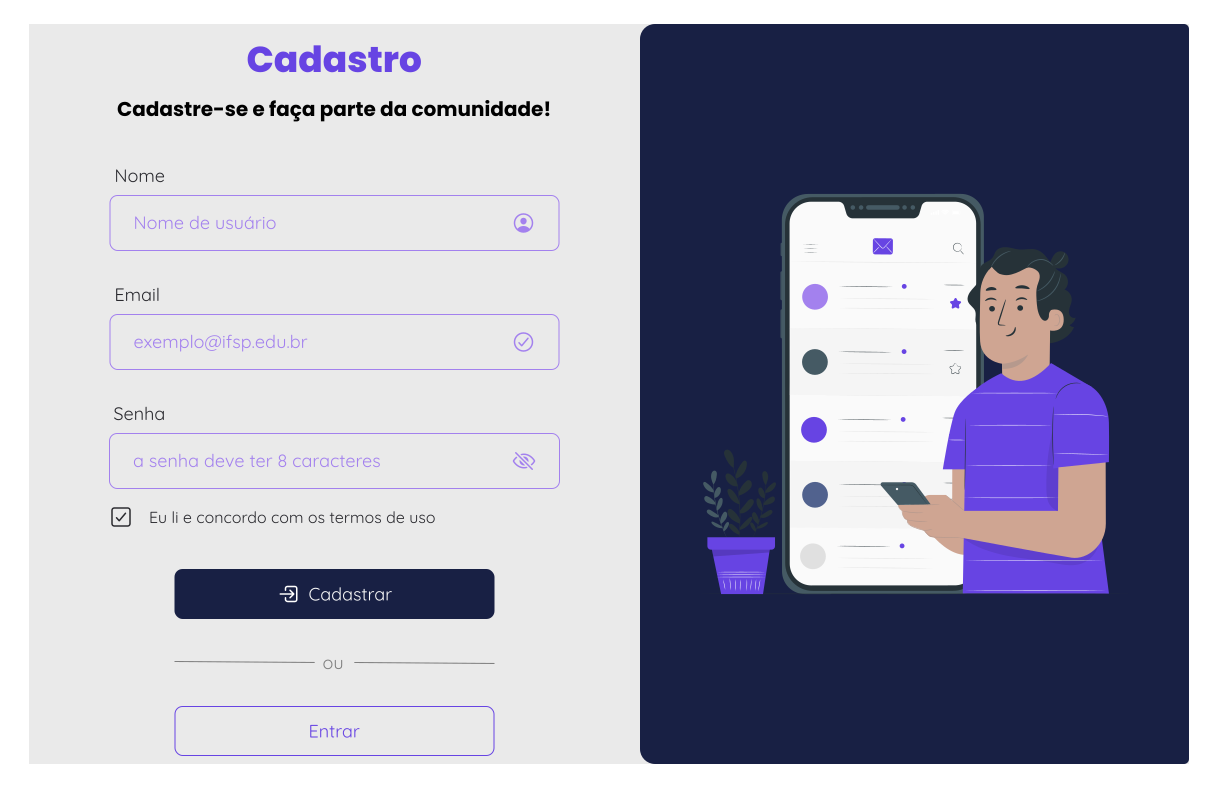
\includegraphics[width=0.8\textwidth]{anexos/Imagens_Prototipo/intro/cadastro.png}
\fonte{Os autores.}
\end{figure}
\FloatBarrier

A \autoref{login} representa a página de login. 

\begin{figure}[htb]
\centering
\caption{\label{login} Página de login}
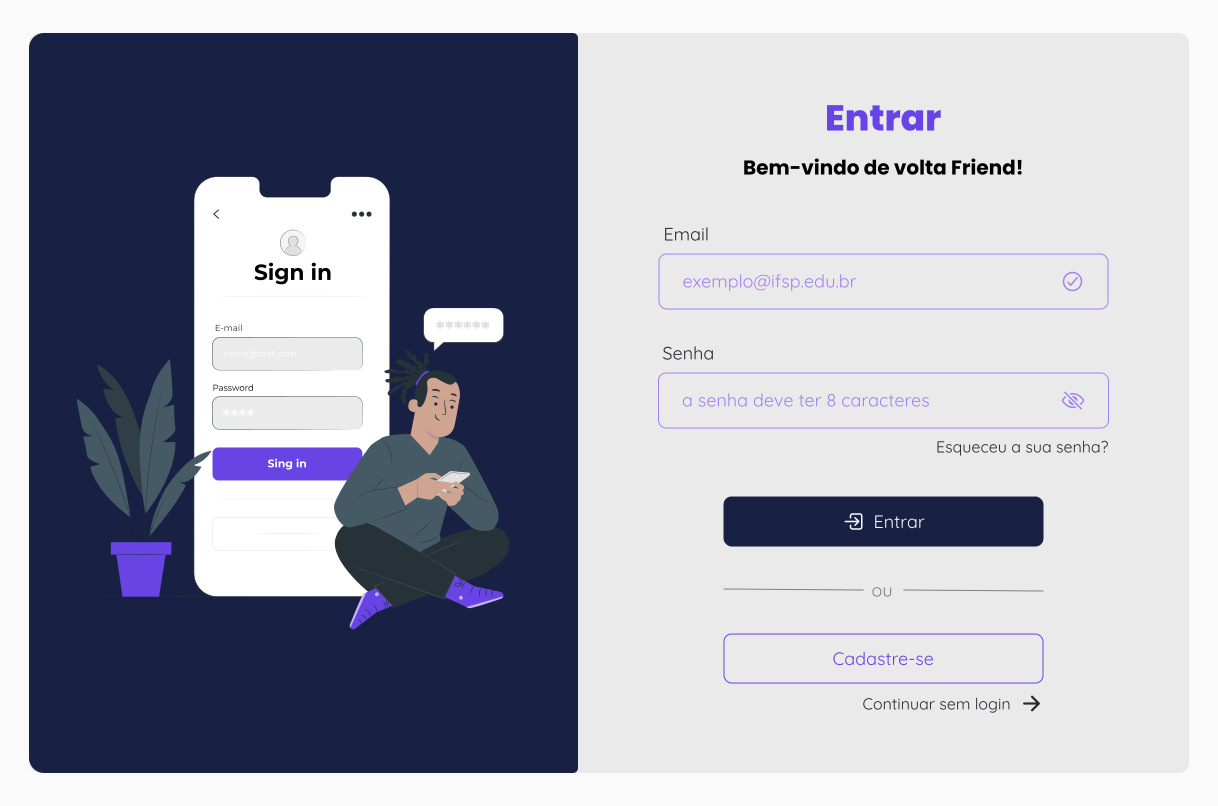
\includegraphics[width=1\textwidth]{anexos/Imagens_Prototipo/intro/login.png}
\fonte{Os autores.}
\end{figure}
\FloatBarrier

A \autoref{sl_perguntas} representa a página de perguntas, nela o \gls{friend} pode navegar por meio do menu superior ou através do filtro de categorias. 

\begin{figure}[htb]
\centering
\caption{\label{sl_perguntas} Página de perguntas}
\includegraphics[width=0.8\textwidth]{anexos/Imagens_Prototipo/sem_login/perguntas.png}
\fonte{Os autores.}
\end{figure}
\FloatBarrier

A \autoref{sl_detalhes_pergunta} representa a página de detalhes da pergunta, nela é possível visualizar as respostas que aquela pergunta recebeu.

\begin{figure}[htb]
\centering
\caption{\label{sl_detalhes_pergunta} Página de detalhes da pergunta}
\includegraphics[width=0.8\textwidth]{anexos/Imagens_Prototipo/sem_login/pergunta_respostas.png}
\fonte{Os autores.}
\end{figure}
\FloatBarrier

A \autoref{sl_detalhes_pergunta-erro} representa um erro gerado quando o \gls{friend} tenta responder à pergunta no modo visitante, dessa forma, são apresentadas as opções de fazer \textit{login} ou fazer cadastro. 

\begin{figure}[htb]
\centering
\caption{\label{sl_detalhes_pergunta-erro} Página de detalhes da pergunta com erro}
\includegraphics[width=0.8\textwidth]{anexos/Imagens_Prototipo/sem_login/pergunta_respostas-erro.png}
\fonte{Os autores.}
\end{figure}
\FloatBarrier

A \autoref{sl_eventos} representa a página de eventos, nela o \gls{friend} pode navegar por meio do menu superior ou através do filtro de categorias. 

\begin{figure}[htb]
\centering
\caption{\label{sl_eventos} Página de eventos}
\includegraphics[width=1\textwidth]{anexos/Imagens_Prototipo/sem_login/eventos.png}
\fonte{Os autores.}
\end{figure}
\FloatBarrier

A \autoref{sl_usuarios} representa a página de usuários.

\begin{figure}[htb]
\centering
\caption{\label{sl_usuarios} Página de usuários}
\includegraphics[width=1\textwidth]{anexos/Imagens_Prototipo/sem_login/usuarios.png}
\fonte{Os autores.}
\end{figure}
\FloatBarrier

%--------------------------------------------------------------
\section{Friend com login}
%--------------------------------------------------------------
Já para o \gls{friend} \textit{logado} no sistema, não há restrições de funcionalidades, então desde que as use com responsabilidade e da forma certa, a aplicação cumprirá o que foi proposto.

Por tanto, a \autoref{cl_perguntas} apresenta a página de perguntas, repare que diferentemente da visão do \gls{friend} sem \textit{login} agora foi inserido o ícone de perfil do usuário, no qual se encontra a internacionalização, configurações do perfil e também a opção de sair.

\begin{figure}[htb]
\centering
\caption{\label{cl_perguntas} Página de perguntas}
\includegraphics[width=0.8\textwidth]{anexos/Imagens_Prototipo/com_login/perguntas.png}
\fonte{Os autores.}
\end{figure}
\FloatBarrier

Quando o \gls{friend} clica em uma pergunta ou em ``Responder'' ele é direcionado à página dessa pergunta como mostra a \autoref{cl_detalhes_pergunta}, nela ele pode encontrar as respostas já fornecidas por outros membros da comunidade, obter mais informações sobre a pergunta (no caso dela ter imagem), assim como também pode deixar a sua contribuição.

\begin{figure}[htb]
\centering
\caption{\label{cl_detalhes_pergunta} Página de detalhes da pergunta}
\includegraphics[width=0.8\textwidth]{anexos/Imagens_Prototipo/com_login/detalhes_perguntas.png}
\fonte{Os autores.}
\end{figure}
\FloatBarrier

Caso o \gls{friend} identifique algum comportamento inadequado ou que viole a política da comunidade, ele tem a possibilidade de reportar o ocorrido, como mostra a \autoref{cl_pergunta-reportar_respostas}.

\begin{figure}[htb]
\centering
\caption{\label{cl_pergunta-reportar_respostas} Página de reportar}
\includegraphics[width=0.8\textwidth]{anexos/Imagens_Prototipo/com_login/pergunta-reportar_respostas.png}
\fonte{Os autores.}
\end{figure}
\FloatBarrier

Já a \autoref{cadastro_perguntas} corresponde a página de cadastro de perguntas, nessa tela são apresentados todos os elementos necessários para a sua realização, assim como o manual de uma boa pergunta (\autoref{boapergunta}), elaborado com o intuito de auxiliar o \gls{friend}. 

\begin{figure}[htb]
\centering
\caption{\label{cadastro_perguntas} Página de cadastro de perguntas}
\includegraphics[width=0.8\textwidth]{anexos/Imagens_Prototipo/com_login/cadastro_perguntas.png}
\fonte{Os autores.}
\end{figure}
\FloatBarrier

A \autoref{cl_eventos} representa a página de eventos, repare que outro elemento introduzido foi o botão de ``Criar'', nele o \gls{friend} consegue facilmente ser direcionado a página de criação de um evento ou de uma pergunta.

\begin{figure}[htb]
\centering
\caption{\label{cl_eventos} Página de eventos}
\includegraphics[width=0.8\textwidth]{anexos/Imagens_Prototipo/com_login/eventos.png}
\fonte{Os autores.}
\end{figure}
\FloatBarrier

A \autoref{cl_detalhes_evento} representa a página de detalhes do evento, nela é possível visualizar mais detalhes do evento.

\begin{figure}[htb]
\centering
\caption{\label{cl_detalhes_evento} Página de detalhes do evento}
\includegraphics[width=0.8\textwidth]{anexos/Imagens_Prototipo/com_login/detalhes_eventos.png}
\fonte{Os autores.}
\end{figure}
\FloatBarrier

Já a \autoref{cadastro_evento} corresponde a página de cadastro de eventos, nessa tela são pedidos informações importantes para realizar o cadastro. 

\begin{figure}[htb]
\centering
\caption{\label{cadastro_evento} Página de cadastro de eventos}
\includegraphics[width=0.8\textwidth]{anexos/Imagens_Prototipo/com_login/cadastro_eventos.png}
\fonte{Os autores.}
\end{figure}
\FloatBarrier

A \autoref{cl_usuarios} representa a página de usuários, nela o \gls{friend} pode visualizar ou pesquisar por usuários da comunidade. 

\begin{figure}[htb]
\centering
\caption{\label{cl_usuarios} Página de usuários}
\includegraphics[width=0.8\textwidth]{anexos/Imagens_Prototipo/com_login/usuarios.png}
\fonte{Os autores.}
\end{figure}
\FloatBarrier

A \autoref{perfil_usuario} representa a página de perfil do usuário, nela são encontrados mais elementos sobre o \gls{friend}, como seus dados, a \gls{gamificação}, suas contribuições, ou seja, suas perguntas, suas respostas e os eventos que publicou. 

\begin{figure}[htb]
\centering
\caption{\label{perfil_usuario} Página de perfil do usuário}
\includegraphics[width=0.8\textwidth]{anexos/Imagens_Prototipo/com_login/perfil_usuario.png}
\fonte{Os autores.}
\end{figure}
\FloatBarrier

Clicando no botão ``Editar perfil'' o \gls{friend} é direcionado a página para editar o perfil (\autoref{editar_perfil}).

\begin{figure}[htb]
\centering
\caption{\label{editar_perfil} Página de atualização de perfil}
\includegraphics[width=0.8\textwidth]{anexos/Imagens_Prototipo/com_login/editar_perfil.png}
\fonte{Os autores.}
\end{figure}
\FloatBarrier

Vale ressaltar que as páginas prototipadas tem um fim norteador, logo pode ocorrer que alguns elementos não fiquem totalmente iguais. 
\chapter{Atas das Reuniões}
\label{atasReunioes}
%----------------------------------------------------------------------------------

\section{1\textordmasculine bimestre}
\subsection{Planejamento - 15/03/2022}
\noindent Integrantes: Anaí Rojas, Jamilli Gioielli, José Roberto, Julia Romualdo, Kaiky Matsumoto \\
Local: \gls{discord}. \\
Pauta(s): Primeira reunião realizada pela equipe com o objetivo de planejar os passos iniciais do projeto, nela a equipe estabeleceu um contrato social na plataforma \gls{figma} contendo os combinados essenciais para o convívio social entre os componentes da equipe e também iniciou-se um \textsl{board} de ideias iniciais para o projeto.

\subsection{Planejamento/Alinhamento - 17/03/2022}
\noindent Integrantes:\,Anaí Rojas, Jamilli Gioielli, José Roberto, Julia Romualdo, Kaiky Matsumoto \\
Local: \gls{discord}.\\
Pauta(s): Reunião de planejamento e alinhamento, onde o foco da equipe esteve em discutir as ideias pré-selecionadas na reunião anterior para o projeto. Desde este primeiro momento a atenção da equipe se voltava principalmente para uma comunidade de dúvidas entre os estudantes do IF. \\
Para organização das tarefas e da equipe a plataforma \gls{notion}, onde o quadro de \textsl{kanban} se encontra, foi criado e organizado inicialmente. \\
A equipe decidiu inicialmente que realizará reuniões nos dias e horários das janelas entre as aulas, permitidas pela grade curricular.

\subsection{Planejamento/Alinhamento - 18/03/2022}
\noindent Integrantes: Anaí Rojas, Jamilli Gioielli, José Roberto, Julia Romualdo, Kaiky Matsumoto \\
Local: \gls{discord}.\\
Pauta(s): Reunião de planejamento onde a equipe discutiu as tarefas a serem realizadas e discutiu outras ferramentas de organização. \\
Criamos o canal do \gls{youtube}.\\
Realizamos a primeira postagem para o \textsl{blog} da equipe.\\
Amadurecemos ainda mais a ideia da comunidade, pensando em mais funcionalidades para agregar na aplicação e anotando as dúvidas a respeito do tema e do funcionamento.

\subsection{Alinhamento - 21/03/2022}
\noindent Integrantes: Anaí Rojas, Jamilli Gioielli, José Roberto, Julia Romualdo, Kaiky Matsumoto \\
Local: Saguão \acs{ifsp}.\\
Pauta(s): Reunião realizada antes da aula de \acs{pds} para a equipe discutir algumas dúvidas, perspectivas e ideias sobre o projeto, visando otimizar o tempo em sala de aula.

\subsection{Alinhamento - 25/03/2022}
\noindent Integrantes: Anaí Rojas, Jamilli Gioielli, José Roberto, Julia Romualdo, Kaiky Matsumoto \\
Local: \gls{discord}.\\
Pauta(s): Reunião de alinhamento, onde a equipe pesquisou em trabalhos anteriores a formatação do documento da proposta inicial para preparar as etapas. 
Aproveitamos também para melhorar o \textsl{layout} do \textsl{blog} da equipe.

\subsection{Planejamento/Alinhamento - 28/03/2022}
\noindent Integrantes:\,Anaí Rojas, Jamilli Gioielli, José Roberto, Julia Romualdo, Kaiky Matsumoto\\
Local: Laboratório \acs{ifsp}.\\
Pauta(s): Reunião de alinhamento e planejamento, onde a equipe conversou com os orientadores sobre soluções e funcionalidades para a proposta da comunidade. Neste ponto, resolvemos um problema antigo, validar que o usuário seja de fato aluno da instituição, a solução encontrada foi enviar um \textsl{e-mail} de validação para o \textsl{e-mail} institucional do aluno. Foi citado também outra proposta de projeto para a equipe realizar, uma plataforma de controle e gestão financeira. Porém, a equipe optou por seguir na proposta da comunidade.\\
Partimos para as tarefas, iniciando o desenvolvimento de um questionário direcionado aos alunos do instituto para estudar a viabilidade de criação do projeto.\\
Sobre o \textsl{blog}, finalizamos a melhoria de seu \textsl{layout} e definimos que as publicações serão realizadas aos sábados pela manhã.

\subsection{Planejamento/Retrospectiva - 02/04/2022}
\noindent Integrantes:\,Anaí Rojas, Jamilli Gioielli, José Roberto, Julia Romualdo, Kaiky Matsumoto \\
Local: \gls{discord}.\\
Pauta(s): Reunião de retrospectiva e planejamento das atividades, onde revisamos a publicação da semana no \textsl{blog} e as perguntas para a pesquisa de viabilidade. Realizamos a entrega sobre as tecnologias que serão utilizadas no desenvolvimento do projeto no \gls{moodle} da disciplina e definimos duas tarefas: divulgação da pesquisa de viabilidade a partir de segunda-feira para alunos e ex-alunos da instituição e gerenciamento do \textsl{backlog} para cada parte do projeto.

\subsection{Planejamento - 04/04/2022}
\noindent Integrantes:\,Anaí Rojas, Jamilli Gioielli, José Roberto, Julia Romualdo, Kaiky Matsumoto \\
Local: Laboratório \acs{ifsp}.\\
Pauta(s): Reunião de planejamento, onde a equipe após receber as orientações para a apresentação da proposta inicial, organizou as tarefas a serem realizadas por cada componente, organizou a formatação do documento para a proposta inicial e iniciou a divulgação do formulário para pesquisa de viabilidade da proposta.

\subsection{Alinhamento - 09/04/2022}
\noindent Integrantes: Anaí Rojas, Jamilli Gioielli, José Roberto, Julia Romualdo, Kaiky Matsumoto \\
Local: \gls{discord}.\\
Pauta(s): Reunião de alinhamento, onde a equipe se reuniu para realizar as atividades destinadas a apresentação da proposta inicial.

\subsection{Alinhamento - 10/04/2022}
\noindent Integrantes: Anaí Rojas, Jamilli Gioielli, José Roberto, Julia Romualdo, Kaiky Matsumoto \\
Local: \gls{discord}.\\
Pauta(s): Reunião de alinhamento, onde a equipe se reuniu para realizar as atividades destinadas a apresentação da proposta inicial.

\subsection{Retrospectiva - 12/04/2022}
\noindent Integrantes:\,Anaí Rojas, Jamilli Gioielli, José Roberto, Julia Romualdo, Kaiky Matsumoto \\
Local: Biblioteca \acs{ifsp}.\\
Pauta(s): Reunião retrospectiva, onde a equipe analisou como foi o processo para realizar a entrega da proposta inicial, desta forma foram levantados os pontos positivos: todos estarem reunidos em chamada para realizar as tarefas, conseguimos entregar o que era esperado e apesar das dificuldades enfrentadas a apresentação fluiu bem. Os pontos negativos: realizar muitas tarefas no final de semana ficou puxado para a equipe e não ter realizado um ensaio antes da apresentação, como melhoria, queremos marcar mais reuniões com os professores.

\subsection{Planejamento/Alinhamento - 17/04/2022}
\noindent Integrantes: Anaí Rojas, Jamilli Gioielli, José Roberto, Julia Romualdo, Kaiky Matsumoto \\
Local: \gls{discord}.\\
Pauta(s): Reunião de planejamento e alinhamento para a semana, onde a equipe planejou as próximas \textsl{sprints} da \acs{POC} juntamente com os professores e aproveitou para conversar sobre as avaliações das equipes em relação a apresentação da proposta inicial. 

\subsection{Planejamento - 18/04/2022}
\noindent Integrantes:\,Anaí Rojas, Jamilli Gioielli, José Roberto, Julia Romualdo, Kaiky Matsumoto. \\
Local: Laboratório \acs{ifsp}.\\
Pauta(s): Reunião de planejamento onde a equipe criou o \textsl{backlog} do produto com o uso das histórias de usuário e definiu as tarefas da semana, preparando-se para os dois épicos para a \acs{POC}.

\subsection{Alinhamento - 21/04/2022}
\noindent Integrantes: Anaí Rojas, Jamilli Gioielli, José Roberto, Julia Romualdo, Kaiky Matsumoto \\
Local: \gls{discord}.\\
Pauta(s): Reunião de alinhamento, onde a equipe terminou de elaborar as histórias de usuário, definiu as prioridades para a \acs{POC} e votou por meio do \textsl{Planning Poker} - descrito pela metodologia Scrum - para estimarmos os esforços necessários para a conclusão de cada história. Durante as discussões da equipe para a execução desta tarefa, muitos pontos sutis, mas que poderiam ser perigosos no futuro, foram levantados e anotados para discutirmos com os orientadores. 

\subsection{Alinhamento - 25/04/2022}
\noindent Integrantes: Anaí Rojas, Jamilli Gioielli, José Roberto, Julia Romualdo, Kaiky Matsumoto \\
Local: Laboratório \acs{ifsp}.\\
Pauta(s): Reunião de alinhamento onde a equipe conversou com os orientadores sobre as dúvidas levantadas na reunião anterior, durante a elaboração da tarefa de definição das histórias de usuários, apresentou os diagramas de entidade e relacionamento e o diagrama de casos de uso para serem alinhados corretamente. Iniciamos também as configurações para criação do vídeo do \gls{gource}.

\subsection{Alinhamento - 01/05/2022}
\noindent Integrantes: Anaí Rojas, Jamilli Gioielli, José Roberto, Julia Romualdo, Kaiky Matsumoto \\
Local: \gls{discord}.\\
Pauta(s): Reunião de alinhamento onde a equipe finalizou as histórias de usuário com base na discussão realizada em aula com os orientadores, alinhou o fluxo de usuário no sistema, os requisitos funcionais, não funcionais e as regras de negócio. Iniciamos o planejamento para realização da apresentação da \acs{POC} e como orientação dos professores, decidimos deixar para desenvolver o épico de Gestão de Eventos apenas se sobrar tempo. 

\subsection{Alinhamento - 03/05/2022}
\noindent Integrantes: Anaí Rojas, Jamilli Gioielli, José Roberto, Julia Romualdo, Kaiky Matsumoto \\
Local: \gls{discord}. \\
Pauta(s): Realização de tarefas para a \acs{POC}, configurações de ambiente e alinhamento da documentação.

\section{2\textordmasculine bimestre}

\subsection{Retrospectiva - 16/05/2022}
\noindent Integrantes: Anaí Rojas, Jamilli Gioielli, José Roberto, Julia Romualdo, Kaiky Matsumoto \\
Local: Laboratório \acs{ifsp}. \\
Pauta(s): Reunião retrospectiva referente ao desenvolvimento e entrega da \acs{POC}, onde a equipe chegou as seguintes conclusões: do que foi bom, entrega da \acs{api} completa; do que foi ruim, falta de tempo, pois mesmo sabendo como desenvolver um dos requisitos não sobrou tempo para fazer; e um problema enfrentado por nós e pelas outras equipes da turma foi a incerteza e a definição errada que construímos sobre a \acs{POC}, isso gerou uma dificuldade na definição do que era extremamente essencial para a entrega. Como plano de ação, a equipe buscará definir melhor o que é simples e objetivo para as próximas entregas, evitando perca de tempo e desgaste com tarefas que não são prioridade.

\subsection{Planejamento - 29/05/2022}
\noindent Integrantes: Anaí Rojas, Jamilli Gioielli, José Roberto, Julia Romualdo, Kaiky Matsumoto \\
Local: \gls{discord}. \\
Pauta(s): Reunião de planejamento onde a equipe encerrou a \gls{Sprint} que tinha como objetivo melhorar aquilo que tinha sido desenvolvido na \acs{POC} e descreveu as tarefas que foram realizadas por cada membro da equipe.

\subsection{Planejamento - 06/06/2022}
\noindent Integrantes: Anaí Rojas, Jamilli Gioielli, José Roberto, Julia Romualdo, Kaiky Matsumoto \\
Local: Laboratório \acs{ifsp}. \\
Pauta(s): Reunião de planejamento onde a equipe após ser orientada pelos professores definiu os tópicos que serão abordados na apresentação da primeira versão e a partir disso, definiu as tarefas a serem desenvolvidas por cada membro.

\subsection{Planejamento 13/06/2022}
\noindent Integrantes: Anaí Rojas, Jamilli Gioielli, José Roberto, Julia Romualdo, Kaiky Matsumoto \\
Local: \gls{discord}. \\
Pauta(s): Reunião de planejamento onde a equipe conversou e definiu melhor alguns pontos do cadastro, como: definição dos requisitos para uma senha válida e quais domínios de e-mails estarão disponíveis para que o usuário selecione. Como a entrega da primeira versão está prevista para a próxima semana, o objetivo é que até quinta feira esteja tudo documentado e até domingo as tarefas estejam concluídas. 

\noindent Iniciamos uma discussão sobre abordagens para utilizarmos num futuro plano de testes e usabilidade. Também aproveitamos para tirar do caminho uma tarefa pendente que tínhamos, da gravação do vídeo referente a apresentação da \acs{POC}.

\subsection{Retrospectiva 23/06/2022}
\noindent Integrantes: Anaí Rojas, Jamilli Gioielli, José Roberto, Julia Romualdo,\,Kaiky Matsumoto \\
Local: Sala \acs{ifsp}. \\
Reunião retrospectiva onde a equipe teve um momento dinâmico de conversa sobre a entrega e apresentação da primeira versão do sistema. Definiu-se como pontos positivos: a comunicação assíncrona através do \gls{WhatsApp} que ajudou a resolver os imprevistos de maneira mais rápida, a apresentação como um todo e o \textit{feedback} positivos dos professores sobre ela. De pontos negativos: falta de um escopo definido sobre a apresentação,  insegurança sobre o que era realmente esperado, o tempo de apresentação passou um pouco do que era estipulado para cada equipe, os \textit{commits} não frequentes durante o desenvolvimento e as histórias de usuário muito grandes durante a \gls{Sprint}. Em pontos a serem melhorados: alimentar mais o \textit{blog} e o canal do \gls{youtube}, usar o \gls{github} como repositório secundário, ter comunicação transparente sobre o que está acontecendo no projeto e preparar uma estratégia de apresentação de acordo com o que for esperado. E um elogio levantado de maneira geral pela equipe é o empenho e dedicação de todos os integrantes, que querem fazer este projeto da melhor maneira possível para que o sistema realmente seja útil para outros alunos. 

\subsection{Planejamento 26/06/2022}
\noindent Integrantes: Anaí Rojas, Jamilli Gioielli, José Roberto, Julia Romualdo,\,Kaiky Matsumoto \\
Local: \gls{discord}. \\
Reunião de planejamento onde a equipe criou uma \gls{Sprint} com melhorias pequenas e detalhes que pudessem ser realizados sem muito esforço, visto que o tempo hábil a ser investido no projeto estava curto devido as outras disciplinas. Em um segundo momento um \textit{backlog} foi elaborado com detalhes e planejamento dos próximos passos a serem realizados no sistema e da documentação que vão ser usados para criar as próximas \glspl{Sprint} com objetivo de serem executadas durante as férias.

\subsection{Planejamento 23/07/2022}
\noindent Integrantes: Anaí Rojas, Jamilli Gioielli, José Roberto, Julia Romualdo, Kaiky Matsumoto \\
Local: \gls{discord}. \\
Reunião de planejamento onde a equipe mediu quantas semanas restam até a próxima entrega, que pode ser considerada a final e quantas horas cada integrante consegue se dedicar ao projeto diariamente durante o período de férias e de aulas. Com essa métrica foi elaborado um plano de entregas para que toda semana uma entrega pequena seja feita. Por último, os tópicos a serem adicionados na revisão de literatura foram abordados e organizados de forma que façam sentido no escopo do documento.

\subsection{Planejamento 28/07/2022}
\noindent Integrantes: Anaí Rojas, Jamilli Gioielli, José Roberto, Julia Romualdo,\,Kaiky Matsumoto \\
Local: \gls{discord}. \\
Reunião de planejamento onde a equipe elaborou, quebrou e refinou algumas histórias de usuário. Aproveitou-se para definir quais histórias são essenciais para a próxima entrega, para que elas já possam começar a ser desenvolvidas durante as férias. Em um segundo momento uma maior atenção foi dada ao protótipo, pensou-se que a usabilidade do sistema não fazia muito sentido, muitos elementos poderiam ser retirados ou substituídos e por isso uma maior atenção será dada a reorganização do \textit{layout} do sistema. Além disso, as categorias foram definidas nos tópicos: ensino, esportes, estágio, entretenimento, institucional e outros.

\subsection{Planejamento 04/08/2022}
\noindent Integrantes: Anaí Rojas, Jamilli Gioielli, José Roberto, Julia Romualdo, Kaiky Matsumoto \\
Local: \gls{discord}. \\
Reunião de planejamento onde a equipe pesquisou e definiu as alterações principais para o protótipo e consequentemente, \textit{layout} do sistema. Foi definido que as pesquisas iniciais para a revisão de literatura deviam começar no final de semana. E por último, as histórias de usuário foram medidas por meio do \textit{planing poker}.  

\section{3\textordmasculine bimestre}

\subsection{Planejamento 08/08/2022}
\noindent Integrantes: Anaí Rojas, Jamilli Gioielli, José Roberto, Julia Romualdo,\,Kaiky Matsumoto \\
Local: Laboratório \acs{ifsp}. \\
Reunião de planejamento realizada pela equipe com a participação de um dos professores onde a equipe apresentou as mudanças realizadas no \textit{layout} do sistema e discutiu o funcionamento dos filtros por categoria. Além disso, com o tempo restante em aula, a equipe quebrou mais histórias de usuário para que o desenvolvimento seja facilitado o máximo possível.

\subsection{Planejamento/Alinhamento 15/08/2022}
\noindent Integrantes: Anaí Rojas, Jamilli Gioielli, José Roberto, Julia Romualdo, Kaiky Matsumoto \\
Local: Laboratório \acs{ifsp}. \\
Reunião de planejamento e alinhamento onde juntamente com os professores a equipe foi convencida de que precisava implantar um sistemas de denúncias no site para a próxima entrega, por isso trabalhou para que a questão fosse solucionada de forma rápida. Assim, definiu-se que um botão será adicionado ao sistema onde o usuário pode enviar um \textit{ e-mail} aos administradores contendo sua denúncia. 

\section{4\textordmasculine bimestre}
\subsection{Retrospectiva 17/10/2022}
\noindent Integrantes: Anaí Rojas, Jamilli Gioielli, José Roberto, Julia Romualdo, Kaiky Matsumoto \\
Local: Laboratório \acs{ifsp}. \\
Reunião retrospectiva relativa à entrega e apresentação final do projeto, onde foi definido o que foi bom: reuniões menos frequentes e maior foco na realização das tarefas, como muito tempo havia sido dedicado em reuniões de planejamento para definição do \textit{backlog}, economizou-se esse tempo que foi utilizado para desenvolvimento das tarefas. O que poderia melhorar: comunicação assíncrona pelo \gls{WhatsApp}, os quadros no \gls{notion} eram  atualizados mas a equipe falhou na comunicação interna sobre o andamento do projeto durante a semana. O plano de ação definido foi: enviar mensagem no grupo do \gls{WhatsApp} no sábado ou domingo, falando sobre as tarefas desenvolvidas durante a semana.


\chapter{Publicações no blog da equipe}
\label{postsBlog}
%------------------------------------------------------------------

\section{1\textordfeminine \, Semana - 14/03 à 20/03}

\begin{figure}[htb]
\centering
\caption{Logo da equipe Bunka Bytes}
\includegraphics[width=0.3\textwidth]{anexos/Imagens_Blog/LogoBunkaPDS.png}
\fonte{Os autores.}
\end{figure}
\FloatBarrier

Primeiramente, bem vindos à primeira postagem da equipe! O principal objetivo deste blog é dar aos leitores a possibilidade de acompanhar nosso "diário semanal" de desenvolvimento dentro da disciplina de Prática de Desenvolvimento de Sistemas (ou \acs{pds} para os mais íntimos).

Mas antes de dar continuidade ao texto, precisamos apresentá-los a equipe Bunka Bytes, cujo nome é parte inspirado no tema do trabalho anterior (em \acs{tds}), já que este possuía um foco cultural e "Bunka" em japonês significa "cultura"; e outra parte se deve a uma referência/trocadilho com a área de informática, pois falando, é quase como se estivéssemos dizendo "Boom Kabytes". 

Integrantes da equipe:

\begin{itemize}
    \item Anai Rojas
    \item Jamilli Gioielli
    \item José Roberto
    \item Julia Romualdo
    \item Kaiky Matsumoto
\end{itemize}

Dos integrantes, escolhemos a Jamilli como nossa representação de gerente, devido a seus conhecimentos em organização, metodologias e ferramentas de gerenciamento e por sua facilidade comunicativa. 

Tendo isso em vista, nesta primeira semana da disciplina, realizamos três reuniões pela plataforma \gls{discord}, nas quais conhecemos melhor nossos colegas de equipe, fizemos um Contrato Social e criamos um \textsl{Brainstorming} utilizando conceitos de \textsl{Design Thinking} na plataforma \gls{figma}, que ajudou numa melhor visualização das ideias centrais para o projeto.  Também tivemos acesso aos trabalhos anteriores e consultamos dois trabalhos que eram mais semelhantes ao nosso tema principal. 

A partir do \textsl{Brainstorm}, a ideia que mais se consolidou foi a proposta de criação de uma comunidade de \acs{Q/A} e mentorias como forma de apoio aos estudantes do \acs{ifsp}. Pensamos em muitas outras, mas esta acabou sendo nossa favorita, com base nos requisitos da disciplina de \acs{pds}. Portanto, nosso objetivo para a segunda semana é conversar com os professores sobre a ideia e a desenvolver melhor com base nas nossas discussões e dúvidas a serem sanadas.

Por último, ao final dessa semana, criamos um \textsl{e-mail} conjunto para a criação deste \textsl{blog} e o canal no \gls{youtube}, também conseguimos acessar o Subversion, criar um canal no \gls{discord}, uma página de gerenciamento no \gls{notion} e uma logo para a equipe.


 \textbf{Por: Jamilli Gioielli e Julia Romualdo}

\section{2\textordfeminine \, Semana - 21/03 à 27/03}

Estamos de volta, leitor!

No início dessa semana, voltamos às atividades presenciais e tivemos um primeiro contato com a disciplina neste formato. A partir daí, separamos as 5 ideias que mais se destacaram do nosso \textsl{Brainstorm} da semana anterior e as compartilhamos com os professores. Recebemos algumas sugestões sobre a ideia de comunidade e nos foi recomendado documentar as ideias para enviar no ambiente do \gls{moodle} da disciplina. 

Tendo isso em vista, precisamos nos reunir durante os próximos dias para passar a construção dos nossos pensamentos em formato textual e explicativo. Entretanto, enfrentamos algumas dificuldades nesse sentido, estando a maioria delas em torno do curto tempo que temos entre trabalho e escola para fazer as reuniões. Tentamos conversar na hora anterior às aulas, mas percebemos que faltava apenas documentar melhor o que havíamos conversado. Não foi possível realizar isto na escola devido aos problemas de conexão de rede, então optamos por fazermos aos poucos durante a semana e nos reunirmos depois da aula, via \gls{discord}, para revisar o conteúdo. De todo modo, conseguimos fazer a entrega das duas tarefas da semana no \gls{moodle}.

Nossos objetivos para próxima semana são: definir a proposta para o projeto com base no \textsl{feedback} dos professores e planejar melhor nossos dias e horários para reuniões.

\textbf{Por:  Jamilli Gioielli} 

\section{3\textordfeminine \, Semana - 28/03 à 03/04}
Estamos de volta, Bunkers!

Nesta semana, trabalhamos na viabilidade da nossa proposta. Em aula, discutimos com os professores as funcionalidades que a comunidade pode ter, encontramos uma solução para validar os alunos cadastrados nela, enviando um \textsl{e-mail} de confirmação apenas ao \textsl{e-mail} institucional, que é de posse dos alunos, garantindo assim que os usuários sejam apenas alunos do instituto e por fim, falamos também sobre uma segunda proposta da equipe, que os professores gostaram bastante e deram forte impulso em desenvolve-la por atingir um grupo maior de usuários e ser algo que todos precisam cotidianamente, que é um sistema baseado em controlar gastos e auxiliar na organização financeira.

Entretanto, optamos por continuar com a comunidade, a qual batizamos com o nome: \gls{ifriends}, principalmente porque é mais próximo da nossa realidade como alunos do instituto e por não termos experiência em desenvolvimento de aplicações \textsl{mobile}, o modelo que enxergamos ser o ideal para a criação da segunda proposta. E como análise prática da viabilidade do \gls{ifriends}, elaboramos um formulário, via \gls{googleforms}, para no início da próxima semana, enviarmos aos nossos colegas e alunos do instituto com o intuito de investigar se eles fariam uso da comunidade.

Falando agora sobre a nossa organização como equipe, ainda estamos nos adaptando com nossos horários entre estudos, trabalho e locomoção, então nosso foco será realizar reuniões rápidas e objetivas principalmente nos horários disponíveis antes das aulas começarem.

Resumo das atividades de cada membro da equipe:

\begin{itemize}
    \item Anai - Elaborou formulário da pesquisa de viabilidade
    \item Jamilli - Organizou as atividades a serem realizadas pela equipe 
    \item José, Julia e Kaiky - Trabalharam em melhorias de layout e postagens do blog
\end{itemize}

Para a próxima semana a equipe tem como objetivo estudar as tecnologias e linguagens a serem utilizadas no desenvolvimento do projeto, estruturar um \textsl{backlog} para gerenciamento eficiente das atividades, trabalhar na identidade visual e design da marca \gls{ifriends}.    

\textbf{Por: Julia Romualdo}

\section{4\textordfeminine \, Semana - 04/04 à 10/04}
Estamos de volta, Bunkers!

No inicio desta semana, realizamos a pesquisa de viabilidade da nossa proposta inicial da comunidade, para isto, elaboramos um formulário via \gls{googleforms}, que ficou disponível para receber respostas de segunda-feira (04/04) à sexta-feira (08/04) e todos os integrantes da equipe ficaram responsáveis por enviar o endereço de compartilhamento - \textsl{link} - nos grupos de \gls{WhatsApp} para os alunos da instituição - público-alvo da nossa proposta - respondessem a dez perguntas e compartilharem algumas experiências como alunos do \acs{ifsp} que ajudassem a equipe a compreender se a proposta era ou não viável.

Ainda nesta semana, recebemos dos professores as orientações para apresentação da proposta inicial, juntamente com a entrega da documentação e estudo de dois projetos anteriores. Para realização desta tarefa, durante a semana a equipe se organizou da seguinte forma:
\begin{itemize}
    \item Anai -  Criou \textsl{branchmarketing} para a aplicação e estudou o projeto WebLab.
    \item Jamilli - Organizou as atividades a serem realizadas pela equipe e estruturou as documentações.
    \item José - Estudou as tecnologias a serem utilizadas no projeto e também do projeto Monitorando.
    \item Julia - Compilou dados da pesquisa de viabilidade de proposta e estudou o  projeto Monitorando.
    \item Kaiky -  Estudou as tecnologias a serem utilizadas no projeto e também do projeto WebLab.
\end{itemize}
Para a próxima semana a equipe tem como objetivo apresentar a proposta e estudar os \textsl{feedbacks} fornecidos pelos professores e colegas durante a apresentação.

\textbf{Por: Julia Romualdo} 

\section{5\textordfeminine \, Semana - 11/04 à 17/04}
 Estamos de volta, Bunkers!

Iniciamos esta semana com a apresentação da proposta inicial da comunidade \gls{ifriends} aos nossos professores e colegas de classe, dos quais recebemos orientações e \textsl{feedbacks}. Neste mesmo cenário, também participamos da apresentação das outras equipes e compartilhamos nossos \textsl{feedbacks} aos mesmos.

Após a apresentação, a equipe se reuniu na biblioteca do \acs{ifsp} para realizar uma retrospectiva, com o objetivo de avaliar o funcionamento da equipe durante a intensa semana de trabalhos que tivemos para realizar a entrega da proposta inicial. Aproveitamos este momento, para decidir os pontos a serem melhorados na apresentação para realizarmos a gravação e entrega do vídeo da proposta e também ajustamos alguns pontos que faltavam ser encaixados sobre as tecnologias que serão utilizadas no projeto.

Além disso, aproveitamos o feriado para revisar alguns conceitos que tínhamos dúvidas e procurar possíveis melhorias para nossa apresentação e documentação. Uma das coisas que percebemos era que ainda precisávamos validar o arquivo equipe.yaml no yamllint, já que ele não estava sendo refletido na página de Blogs de Trabalhos, por isso aproveitamos para ajustá-lo de acordo com os apontamentos que foram dados pelo validador.

De todo modo, a equipe tem como meta para a próxima semana a atualização das fontes do projeto de acordo com o \textsl{feedback} que será dado pelos demais colegas e pelos professores após a apresentação da proposta. Além disso, pretendemos postar o vídeo da proposta - já com as melhorias - e também entregar nossas avaliações sobre as demais equipes.

Por isso, contamos com os feriados para adiantar o máximo de atividades possíveis e já pensar em alguns itens de \textsl{backlog} para que possamos iniciar a primeira \textsl{sprint} com o cronograma do projeto já bem definido. Pensando nisso também, a equipe não se dividiu como na semana anterior para a execução das tarefas, já que neste primeiro feriado focaremos juntos em tratar das melhorias, estudar as tecnologias propostas e trabalhar no planejamento do projeto.

\textbf{Por: Julia Romualdo e Jamilli Gioielli}

\section{6\textordfeminine \, Semana - 18/04 à 24/04}
Estamos de volta, Bunkers!

Nesta semana, iniciamos a aula de segunda-feira de forma bem produtiva, pois conversamos bastante com os orientadores a respeito das próximas \textsl{sprints} a serem planejadas e executadas pela equipe. Assim partimos para a criação do \textsl{backlog} do produto com o uso das histórias de usuário, depois definimos as tarefas da semana já nos planejando para os três épicos a serem elaborados para a entrega da Prova de Conceito, sendo eles: Gestão de Perguntas, Gestão de respostas e Gestão de Eventos.

Além disso, aproveitamos o feriado de Tiradentes para nos reunirmos através da plataforma \gls{discord}, com o objetivo de terminar a definição das histórias de usuário, neste momento muitos pontos sutis sobre a aplicação, que poderiam se tornar inimigos da equipe futuramente, foram levantados e anotados para discutir com os professores. Também votamos por meio do \textsl{Planning Poker} - descrito pela metodologia \textsl{Scrum} - para entendermos sobre uma estimativa de esforço para que cada história seja concluída. Junto a isso, também podemos elencar alguns requisitos não funcionais e regras de negócio.

Desta forma, as tarefas realizadas pela equipe durante esta semana foram organizadas da seguinte forma:

\begin{itemize}
    \item Anai e Jamilli - Iniciar a prototipagem das telas.
    \item José e Kaiky - Iniciar a modelagem de dados.
    \item Julia - Iniciar os ajustes na documentação.
\end{itemize}

Para a próxima semana, além de dar início as tarefas da \textsl{sprint}, a equipe tem o objetivo de terminar as tarefas de planejamento e apresenta-las aos orientadores para que possamos esclarecer dúvidas e saber os pontos a serem melhorados.

\textbf{Por: Julia Romualdo}

\section{7\textordfeminine \, Semana - 25/04 à 01/05}
Estamos de volta, Bunkers!

Iniciamos esta semana validando com os professores as atividades que a equipe esteve realizando desde a semana passada, fomos orientados quanto a melhor organização dos tópicos do documento, a remover algumas histórias dos épicos para a \acs{POC}, - pois alguns pontos estavam fugindo da ideia da \acs{POC}, que é provar que o conceito principal, ou seja, o fluxo principal da aplicação está funcionando -, a realizar a entrega do épico de Gestão de Eventos, na \acs{POC}, apenas se sobrar tempo, ajustar o diagrama de entidade relacionamento e o diagrama de casos de uso. Aproveitamos este momento ainda em aula para iniciar as configurações do \gls{gource}, pensando em futuras entregas da disciplina.

Devido ao final de bimestre, a equipe esteve ocupada com as atividades de outras disciplinas e não conversou muito durante esta semana, mas os componentes continuaram no desenvolvimento - visando o termino - das atividades propostas na semana passada, organizadas da seguinte forma:
\begin{itemize}
    \item Anai - Terminar a prototipagem das telas.
    \item José e Kaiky - Ajustar a modelagem de dados.
    \item Jamilli - Terminar a prototipagem das telas e ajustar os tópicos de gerenciamento e metodologias da documentação. 
    \item Julia - Adicionar os apêndices na documentação e pesquisar sobre o \gls{gource}.
\end{itemize}
\noindent Para a próxima semana a equipe tem como objetivo desenvolver a Prova de Conceito e a documentação relacionada a mesma.

\textbf{Por: Julia Romualdo}

\section{8\textordfeminine \, Semana - 02/05 à 08/05}
Estamos de volta, Bunkers!

Esta semana devido a problemas na infraestrutura do encanamento do campus \acs{ifsp} não tivemos aulas de maneira presencial e poucos professores ministraram no formato \acs{ead}, aproveitamos então o plantão de segunda-feira com os orientadores para alinharmos o fluxo de usuário e o protótipo para a \acs{POC}. No decorrer da semana utilizamos os horários que seriam destinados às aulas para realizarmos as tarefas de desenvolvimento da \acs{POC} (desenvolvimento, documentação e apresentação), para isto a equipe ficou organizada da seguinte maneira: 
\begin{itemize}
    \item Anai - Realizar ajustes finais no prototipo e ajustar a documentação.
    \item José e Jamilli - Configurar o ambiente e desenvolver o \gls{front-end}
    \item Julia - Realizar ajustes na documentação e gerar vídeo do \gls{gource}.
    \item Kaiky - Configurar o ambiente e desenvolver \gls{back-end} e Banco de Dados.
\end{itemize}
\noindent Para a próxima semana a equipe tem como objetivo apresentar a Prova de Conceito e realizar reunião retrospectiva sobre o desenvolvimento da \gls{POC}.

\textbf{Por: Julia Romualdo}

\section{9\textordfeminine \, Semana - 09/05 à 15/05}
Estamos de volta, Bunkers!

Iniciamos esta semana com a apresentação da Prova de Conceito para a turma e orientadores, e devemos dizer que nosso maior inimigo para esta entrega com certeza foi o tempo, pois deixamos de cumprir alguns requisitos da bíblia do Ivan porque nos faltou tempo hábil para concluir alguns tópicos ali estipulados. Ainda assim, acreditamos que conseguimos demonstrar que o fluxo principal da nossa aplicação estava funcionando. 

Por outro lado, pudemos cumprir grande parte dos requisitos necessários para as entregas do primeiro bimestre, faltando apenas nossa planilha de avaliação da equipe, que foi postada no \gls{svn} nessa semana, um pouco tarde devido a um imprevisto ocorrido com o sistema (que ficou fora do ar durante algumas horas). 

A equipe tinha como um dos objetivos para essa semana a realização da reunião retrospectiva referente ao desenvolvimento da \gls{POC}, porém devido a alta demanda que as outras disciplinas exigiram durante a semana - provas, apresentações e outras atividades -, não encontramos um bom momento para nos reunirmos, ficando isso como uma meta para a próxima semana, juntamente com o planejamento para as próximas etapas do desenvolvimento do \gls{ifriends}. Além disso, precisamos atualizar nosso canal no \gls{youtube} com os vídeos para o segundo bimestre, visto que não conseguimos gravá-los e editá-los até o momento. 

\textbf{Por: Julia Romualdo e Jamilli Gioielli}

\section{10\textordfeminine \, Semana - 16/05 à 22/05}
Estamos de volta, Bunkers!

Podendo respirar um pouco mais após a intensa semana de entrega de atividades que tivemos durante a semana passada, iniciamos os trabalhos novamente com a reunião de retrospectiva referente a entrega da \gls{POC}, com isso chegamos as seguintes conclusões: do que foi bom, consideramos a entrega da \acs{api} completa;  para o que foi ruim, por outro lado, consideramos a falta de tempo, pois por mais que soubéssemos como desenvolver um requisito, como a internacionalização ou o vídeo de demonstração, não sobrou tempo para fazer; e por último, outro problema, enfrentado não apenas por nossa equipe mas de maneira geral na turma, foi a incerteza e a definição errada que construímos sobre a \gls{POC} a partir de experiências anteriores, por isso percebemos que não conseguimos definir o que seria extremamente essencial para essa entrega e pode ser que tenhamos focado mais em coisas adicionais do que no principal. Assim, como plano de ação escolhemos que precisamos definir melhor o que é simples e objetivo para nossas entregas, para evitar que tenhamos confusões desnecessárias que acabem dificultando a entregarmos o que era necessário.

Os professores também realizaram alguns apontamentos a partir das nossas entregas relativas do primeiro bimestres, para que possamos realizar os alinhamentos necessários, tais como: representar o \gls{heroku} na arquitetura, postar os vídeos da apresentação da \gls{POC} no \gls{youtube}, realizar \textit{commits} com mais frequência e enviar os arquivos do \LaTeX que estamos usando no Overleaf.

Além disso, os professores separaram uma parte da aula para assistirmos a alguns projetos dos alunos da turma 231 em \acs{pji}, e permitiu que fizemos apontamentos e sugestões para os colegas sobre suas ideias.

Tendo realizado esses dois momentos de alinhamento a equipe documentou tudo, organizou as tarefas e ajustes que deveriam ser realizados durante a semana e partimos para os ajustes. Conseguimos enviar e ajustar o que faltava para o primeiro bimestre, como a questão do \gls{gource} e ainda incluímos alguns requisitos que faltavam na aplicação e na \gls{api} (como a inclusão do \textit{Swagger UI} e criptografia da autenticação). Como a próxima semana será de conselhos de classe, a equipe espera poder trabalhar mais no projeto e dar continuidade no desenvolvimento do mesmo, além de reavaliarmos o que for necessário conforme os demais \textit{feedbacks} dos professores (que ainda serão feitos sobre a \acs{POC}).

\textbf{Por: Julia Romualdo e Jamilli Gioielli}

\section{Como utilizar o Yamllint: validador de arquivos .yaml}

Um dos primeiros itens necessários para iniciar os trabalhos na disciplina de \acs{pds} é  que "após a criação da pasta no repositório \href{https://dicas.ivanfm.com/programacao/scm/controle-de-versao/subversion.html}{Subversion} um arquivo \textbf{equipe.yaml} deve ser criado com os dados da equipe e projeto de acordo com modelo no repositório". Estes dados nada mais são do que aqueles existentes na página \href{https://dicas.ivanfm.com/aulas/blogs-de-trabalhos.html}{Blogs de Trabalhos do Dicas Ivan}, mas para que os trabalhos criados sejam expostos nesta página é preciso seguir alguns critérios na criação do arquivo, e o primeiro deles é a utilização de um validador de arquivos com extensão \textit{.yaml}, isto é, o \href{https://yamllint.readthedocs.io/en/stable/quickstart.html}{yamllint}.

\begin{figure}[htb]
\centering
\caption{\label{Yamillint} Logo Yamillint}
\includesvg[inkscapelatex=false,width=0.3\textwidth]{anexos/Imagens_Blog/yamillint.svg}
\fonte{Icons For Free.com}
\end{figure}
\FloatBarrier

Diante da dificuldade de alguns colegas em validar o arquivo e após fazer algumas pesquisas sobre o validador, percebi que a maior parte dos conteúdos sobre o assunto está em inglês e, arquivos dessa natureza possuem muitas especificações minuciosas para serem validadas, e muitas vezes a documentação do \gls{Yamllint} não as deixa tão claras ao leitor. Por isso, resolvi compartilhar um pouco do que entendi sobre o processo de validação do arquivo, o que inclui a instalação do validador, erros comuns após a validação e a espera até que o projeto apareça na página de \href{https://dicas.ivanfm.com/aulas/blogs-de-trabalhos.html}{Blogs de Trabalhos}.\\

\textbf{O que é o yamllint e por que devo validar um arquivo .yaml?}

Segundo a documentação do \gls{Yamllint}, o validador é inspirado no \textit{\href{https://eslint.org/}{eslint}} do JavaScript, uma ferramenta para análise \textbf{estática do código}. Isso quer dizer que seu objetivo é acusar erros (de programação e de estilo), \textit{bugs} e construções suspeitas sem precisar executar o programa. Ou seja, a análise estática de um validador tem como objetivo trazer uma lista de erros, \textit{warnings} e pontos de melhorias do seu código. 

O que o \gls{Yamllint} faz, basicamente, é este processo de \textit{linting}/análise estática do conteúdo presente em um arquivo .yaml (ou .yml), procurando, não só problemas de sintaxe, como estranhezas e problemas estilísticos. 

Ademais, a linguagem utilizada nesses arquivos, o YAML, é uma "linguagem de serialização de dados" e por isso é muito usada para arquivos de configuração, pois gerenciar configurações de um projeto é importante para manter a consistência do seu sistema e para documentar mudanças nas aplicações - mas isso é assunto pra outro \textit{post}.

No final, o que você precisa saber é que a formatação do seu arquivo é necessária para que o sistema que vai "lê-lo" entenda corretamente as instruções que você deseja passar. Veja algumas coisas importantes sobre a formatação de arquivos.yaml:

\begin{itemize}
    \item O YAML utiliza recuo no estilo \gls{Python} para alinhamento;
    \item Caracteres de tabulação (os chamados "$\backslash$t" ou apenas "TAB")  não são permitidos, por isso utilize espaços em branco;
    \item A forma que os espaços em branco estão dispostos faz diferença na formatação do arquivo e pode apontar erros no validador. Por exemplo: esquecer de colocar um espaço após o caractere ":";
    \item Não há símbolos de formatos comuns, como chaves, colchetes, tags de fechamento, etc;
    \item Os arquivos .yaml são estruturados em mapas ou listas;
    \item As listas têm ordem específica e sua sequência começa com um traço (-) seguido de um espaço.
\end{itemize}

Existem outras coisas a se atentar, mas isso você vai descobrir quando rodar o \gls{Yamllint}. Se quiser saber mais sobre o YAML, recomendo ler \href{https://www.redhat.com/pt-br/topics/automation/what-is-yaml}{este artigo da Red Hat} (tirei algumas coisinhas de lá).\\

\textbf{Como instalar o Yamllint?}

Antes de começar a falar da instalação propriamente dita, considerando que você esteja utilizando o sistema operacional \textbf{Windows}, é importante que você \textbf{se certifique se possui o} \href{https://nodejs.org/en/}{Node.js} (com npm) \textbf{ou o} \href{https://python.org.br/instalacao-windows/}{Python} (com o pip) instalados em sua máquina. Caso esteja utilizando algum sistema operacional baseado em \textbf{\href{https://www.tecmundo.com.br/macos/10556-unix-o-pai-de-todos-os-sistemas-operacionais.htm}{Unix}}, você pode verificar se possui o gerenciador de pacotes mais utilizado nele e seguir as orientações da documentação do \href{https://yamllint.readthedocs.io/en/stable/quickstart.html}{yamllint} para instalar; ou utilizar o \gls{Python} mesmo (também funcionará). Mas, se preferir um caminho alternativo, siga as próximas instruções.\\


\textbf{Em sistemas tipo Unix (alternativa)}

\begin{enumerate}
  \item Primeiro, abra seu terminal Bash e verifique já se possui, na sua pasta \$HOME, o arquivo \textbf{.bash\_profile} (é nele que ficam suas variáveis de ambiente), com o comando: 
    \lstset{language=Fortran,
             basicstyle=\ttfamily\small
    }
        \begin{lstlisting}
            open $HOME/.bash_profile; 
        \end{lstlisting}
  
  \item Caso ele não exista, crie-o na sua pasta de usuário e depois siga os passos para a instalação do gerenciador de pacotes \href{https://brew.sh/index_pt-br}{Homebrew};
  
  \item Dependendo do seu tipo de \acs{SO}, pode ser que o comando: \textbf{brew} não funcione após a instalação, isso acontece porque você precisa criar uma variável de ambiente para ele no seu arquivo .bash\_profile;
  
  \item Para isso, se o próprio instalador não lhe alertar sobre os próximos passos, insira com o comando:  
    \lstset{language=Fortran,
                 basicstyle=\ttfamily\small,
                 showstringspaces=false
        }
        \begin{lstlisting} 
echo 'eval "$(/home/linuxbrew/.linuxbrew/bin/brew shellenv)"'
>> $HOME/.bash_profile
        \end{lstlisting}
        
  \item Depois, insira o comando para atualizar o arquivo
    \lstset{language=Fortran,
             basicstyle=\ttfamily\small
    }
        \begin{lstlisting} 
            source \$HOME/.bash\_profile 
        \end{lstlisting}
        
  \item Agora, basta instalar o yamllint com o comando 
    \lstset{language=Fortran,
            basicstyle=\ttfamily\small
        }
        \begin{lstlisting} 
            brew install yamllint. 
        \end{lstlisting}
  
\end{enumerate}

Dica: se o sistema for muito rebelde e não reconhecer os comandos, tente fechar e abrir novamente o terminal após a instalação. Para ter mais certeza se a variável foi inserida, abra seu arquivo .bash\_profile e verifique se ela está lá. Veja mais dicas de instalação \href{https://livreeaberto.com/homebrew-linux}{aqui}. \\

\textbf{No Windows}

Antes, já deixe seu Prompt de Comando/cmd aberto e vamos lá!

Dica: para essas instalações, prefira utilizar o \acs{cmd} (executando como administrador) ao invés do \textit{Windows PowerShell}, pois o segundo apresentou um erro inesperado durante a instalação do pacote.

\textbf{Para usuários de Node.js}
\begin{enumerate}
  \item Baixar o pacote via 
    \lstset{language=Fortran,
             basicstyle=\ttfamily\small,
             showstringspaces=false
    }
        \begin{lstlisting} 
            npm install -g yaml-lint
        \end{lstlisting}
  \item Verificar se a instalação foi feita com sucesso inserindo o comando
    \lstset{language=Fortran,
             basicstyle=\ttfamily\small,
             showstringspaces=false
    }
        \begin{lstlisting} 
            yammlint -v ou yammlint --version
        \end{lstlisting}  
\end{enumerate}

"\textbf{Obs.:} Nesse caso, você deve tomar cuidado se seu arquivo constar como válido, mesmo não estando, pois a versão do yamllint para \gls{Node.js}, até este momento, vem \href{https://github.com/rasshofer/yaml-lint/issues/31}{apresentando algumas instabilidades} que ainda estão sendo corrigidas. Por isso, tente atualizar sempre para a versão mais recente ou prefira utilizar o \gls{Python}"

\textbf{Para usuários de Python}
\begin{enumerate}
  \item Instale a última versão do gerenciador de pacotes pip, com o comando
    \lstset{language=Fortran,
             basicstyle=\ttfamily\small,
             showstringspaces=false
    }
        \begin{lstlisting} 
            pip install yamllint
        \end{lstlisting}
        depois, verifique a instalação foi inserido o comando
    \lstset{language=Fortran,
             basicstyle=\ttfamily\small,
             showstringspaces=false
    }
        \begin{lstlisting} 
            yamllint -v ou yamllint --version
        \end{lstlisting}
\end{enumerate}

\textbf{Obs.:} É melhor fazer a instalação global ao invés de dentro da pasta usuário, por isso, pode ser que utilizar o parâmetro \textbf{--user} na instalação cause instabilidades para rodar em outros lugares.

\textbf{Como funciona a validação}

Começar a validar é um processo muito simples, basta dar o comando, no mesmo diretório em que seu arquivo está, 
\lstset{language=Fortran,
             basicstyle=\ttfamily\small,
             showstringspaces=false
    }
        \begin{lstlisting} 
            yamllint equipe.yaml
        \end{lstlisting}
O grande problema, na realidade, é descobrir o que deu de errado com ele. É bem provável que você encontre algo assim:

\begin{figure}[htb]
\centering
\caption{Diretório}
\includegraphics[width=0.8\textwidth]{anexos/Imagens_Blog/diretorio.png}
\fonte{yamllint docs.}
\end{figure}
\FloatBarrier

\textbf{Obs.:} Antes, é legal que você tenha olhado os arquivos das outras equipes que conseguiram validar o equipe.yaml, assim você consegue entender melhor como é a estrutura do arquivo. Se preferir baixar o nosso, é só acessar \href{https://svn.spo.ifsp.edu.br/svn/a6pgp//A2022-PDS-SEG/Bunka_Bytes/equipe.yaml}{aqui}, mas também olhe lá no \href{https://dicas.ivanfm.com/aulas/blogs-de-trabalhos.html}{Blog de Trabalhos} os que já estão validados (é só clicar no \textit{link} chamado "\acs{svn}" dos projetos).

Para entender melhor essas mensagens, recomendo que leia também as regras dispostas na documentação do \gls{Yamllint}, lá você vai encontrar o que significa cada erro/\textit{warning} gerado nesse \textit{log}, além de situações em que a estrutura disposta falhe ou passe nos testes. Porém, existem alguns erros comuns que pode ser que você se confunda mais caso leia a documentação. Alguns deles são:

\begin{itemize}
    \item \textbf{Erro - Trailling spaces:} esse erro acontece quando você não remove o espaço depois da última palavra de uma linha. Por isso, fique atento aos números a direita do \textit{log}, eles mostram em qual linha está aquele erro. O cursor precisaria estar "colado" no número 2 para que não apontasse o erro de \textit{trailling spaces} Por exemplo:
        \begin{figure}[htb]
        \centering
        \caption{Erro - \textit{Trailling spaces}}
        \includegraphics[width=0.4\textwidth]{anexos/Imagens_Blog/erro1.png}
        \fonte{Os autores.}
        \end{figure}
        \FloatBarrier
    
    \item \textbf{Erro - no new line at the end of file: } nesse caso você precisa se certificar de que a última linha do seu arquivo é uma linha em branco. Aqui percebemos que a linha 15 é a última linha do arquivo que está em branco. Dessa maneira:
    \begin{figure}[htb]
        \centering
        \caption{Erro - \textit{no new line at the end of file}}
        \includegraphics[width=0.4\textwidth]{anexos/Imagens_Blog/erro2.png}
        \fonte{Os autores.}
        \end{figure}
        \FloatBarrier
    
    \item \textbf{Erro - line too long (X > 80 characters):}  esse erro indica que as linhas de um arquivo .yaml não podem ter mais do 80 caracteres, então se você se deparar com ele, quer dizer que no lugar do "X" estará a quantidade de caracteres daquela linha, sendo essa maior do que 80. Uma dica para isso é quebrar as linhas do texto dando alguns espaços aqui e ali, e não fazer um texto corrido de uma vez (mas cuidado com as monografias).
    
    \item \textbf{Erro - found character '$\backslash$t' that cannot start any token (syntax):} aqui você deve se lembrar lá de cima quando falei sobre a formatação do arquivo, pois esse erro é devido ao uso de tabulação em alguma linha do seu equipe.yaml. 
\end{itemize}

\textbf{Dicas extras e considerações finais}
Uma coisa muito importante a se atentar é o cuidado com os caracteres especiais, pois pode ser que seu arquivo lá no \acs{svn} apareça de um jeito estranho, mais ou menos assim:

\begin{figure}[htb]
        \centering
        \caption{Cuidado}
        \includegraphics[width=0.7\textwidth]{anexos/Imagens_Blog/cuidados.png}
        \fonte{Os autores.}
        \end{figure}
        \FloatBarrier

Isso geralmente acontece pelo \textit{Unicode} do seu arquivo não ser \textbf{UTF-8}. Por isso, ao salvar o arquivo, verifique se a codificação dele está no padrão esperado.

Outra coisa importante de se saber é se \textbf{seu arquivo só vai ser atualizado na página do Dicas Ivan, quando o site for recompilado, o que ocorre a cada dois dias}. Então, fique tranquilo se a atualização não for imediata: é normal. 

Uma dica é sempre verificar o \textit{log} do equipes.yaml, para ver quando/se a compilação já foi feita. Aliás, lá você vai perceber o mesmo tipo de validação que ocorre no \gls{Yamllint}, pois os arquivos que não foram compilados possuem seus erros logo abaixo.

Por último, não esqueça: o Google é seu amigo, se não encontrar algum erro super estranho na documentação, copie-o e cole-o no Google, pode ser que com um pouquinho de garimpo, você encontre a solução que procura.

Por hoje é isso pessoal, se tivermos mais dicas e relacionados para compartilhar com vocês, fiquem atentos nas próximas postagens.

Até mais! :) 

\textbf{Fontes:}

\noindent\href{https://pt.stackoverflow.com/questions/330821/o-que-significa-executar-lint-no-código}{https://pt.stackoverflow.com/questions/330821/o-que-significa-executar-lint-no-código}

\noindent\href{https://yamllint.readthedocs.io/en/stable/}{https://yamllint.readthedocs.io/en/stable/}

\noindent\href{https://www.redhat.com/pt-br/topics/automation/what-is-configuration-management}{https://www.redhat.com/pt-br/topics/automation/what-is-configuration-management}

\noindent\href{https://www.redhat.com/pt-br/topics/automation/what-is-yaml}{https://www.redhat.com/pt-br/topics/automation/what-is-yaml}

\section{Gerando o Vídeo do Gource}
Olá, Bunkers!\\
Estamos aqui hoje com a missão de ajudar vocês a gerar o vídeo no famoso \gls{gource}. Nosso objetivo principal com este \textit{post} é compilar o máximo de informações possíveis de forma simples e objetiva em um único lugar para que vocês não precisem ficar garimpando pedacinhos de informação em diversos \textit{sites} para cumprir uma tarefa que não é difícil.

\textbf{Primeiramente, o que é o Gource?}

O \gls{gource}, nada mais é do que uma ferramenta que permite visualizar o desenvolvimento de um \textit{software} a partir dos \textit{commits} realizados em um repositório (no nosso caso o \acs{svn}) criando um gráfico em formato de árvore.
Um dos requisitos da disciplina de \acs{pds} é que a cada \underline{bimestre, entrega e apresentação feita}, deve ser publicado no canal do YouTube da equipe o vídeo gerado no Gource. 

Segundo a \href{https://dicas.ivanfm.com/programacao/scm/controle-de-versao/gource.html}{bíblia do Ivan}, o vídeo do \gls{gource} deve cumprir as seguintes configurações:
\begin{itemize}
    \item Alterar os userid do repositório por nomes dos participantes;
    \item Colocar uma imagem distinta e especifica para cada usuário;
    \item Utilizar opção \textbf{–key};
    \item Utilizar as opções de \textit{caption} para registrar as principais mudanças feitas no repositório;
    \item Os vídeos devem ter no máximo 1 minuto para cada bimestre; 
\end{itemize}

\textbf{Borá lá trabalhar}

\textbf{1. Instalação}

Para instalar o \gls{gource} é só clicar \href{https://github.com/acaudwell/Gource/releases/download/gource-0.47/gource-0.47.win64-setup.exe}{aqui} (pode confiar que não é vírus).

Use \href{https://www.youtube.com/watch?v=WMEyeu1FKhw}{este tutorial} encontrado no \gls{youtube} para instalar o \textit{ffmpeg}, ele serve para converter o vídeo em .mp4, vamos entender isso melhor mais pra frente.

\textbf{Dica:} É importante que você verifique se as variáveis de ambiente estão devidamente configuradas, caso contrário o terminal irá reclamar quando você começar a rodar os comandos.\\

\textbf{2. Testando 1,2,3}

Clone o repositório \acs{svn} da sua equipe e cole na área de trabalho ou em uma pasta de fácil acesso, faça o passo a passo localmente, nunca dentro do repositório oficial da disciplina.

Abra o terminal local ou cmd: para isso, aperte SHIFT + Botão direito do mouse e vá até a opção "Abrir o PowerShell aqui" ou "Abrir janela de comando aqui".

\begin{figure}[htb]
        \centering
        \caption{Exemplo de como abrir o terminal}
        \includegraphics[width=0.4\textwidth]{anexos/Imagens_Blog/exemplo_abrir_terminal.png}
        \fonte{Os autores.}
        \end{figure}
        \FloatBarrier

Digite \textbf{gource} e aperte Enter

Apareceu um vídeozinho?????? 

Boooa, o \gls{gource} foi instalado corretamente, mas como alegria de Ifiano dura pouco, aperte ESC para sair pois ainda faltam os requisitos da bíblia.\\

\textbf{3. Alterando o log}

Vamos precisar criar um log, para isso execute o seguinte comando usando o nome da sua equipe:
\lstset{language=Fortran,
             basicstyle=\ttfamily\small,
             showstringspaces=false
    }
        \begin{lstlisting} 
            --output-custom-log BunkaBytes
        \end{lstlisting}
        
Após executar o comando, volte na pasta clonada e veja que um arquivo foi criado.

\begin{figure}[htb]
        \centering
        \caption{Arquivo de caption}
        \includegraphics[width=0.3\textwidth]{anexos/Imagens_Blog/arquivo_log.png}
        \fonte{Os autores.}
        \end{figure}
        \FloatBarrier

Abra este arquivo em um editor de texto de sua preferência e altere o prontuário correspondente a cada componente da equipe por seu primeiro nome, então vamos disso:

\noindent 1649709679|sp1234567|A|/A2022-PDS-SEG/Bunka\_Bytes/Documentos/AnaliseProjetos.pdf \\
\noindent 1649709679|sp7654321|A|/A2022-PDS-SEG/Bunka\_Bytes/Documento/PropostaInicial.pdf

Para isso:

\noindent 1649709679|Anai|A|/A2022-PDS-SEG/Bunka\_Bytes/Documentos/AnaliseProjetos.pdf \\
\noindent 1649709679|Jose|A|/A2022-PDS-SEG/Bunka\_Bytes/Documento/PropostaInicial.pdf

\textbf{Dica:} No bloco de notas padrão do \textbf{Windows}, use o Ctrl+H para localizar e substituir as linhas mais rápido.

Não é obrigatório, mas para você que prefere ir verificando se as coisas estão acontecendo certinho conforme estão sendo desenvolvidas, rode o seguinte comando para começar a ver a mágica acontecendo - lembre-se de que é com o nome da sua equipe:

\lstset{language=Fortran,
             basicstyle=\ttfamily\small,
             showstringspaces=false
    }
        \begin{lstlisting} 
            gource BunkaBytes
        \end{lstlisting}
        
\textbf{4. Colocando vossos belos rostos no vídeo}

Crie uma pasta "Imagens", "Avatares" ou algo do tipo dentro do seu repositório clonado e coloque dentro dela uma foto correspondente a cada membro da equipe, recomendamos que utilizem o formato png ou jpeg. O nome da imagem deve ser idêntico ao nome que foi inserido anteriormente no \textit{log}. 

Execute o seguinte código para verificar se funcionou:

\lstset{language=Fortran,
             basicstyle=\ttfamily\small,
             showstringspaces=false
    }
        \begin{lstlisting} 
    gource --output-custom-log BunkaBytes --key --user-dir Imagens
        \end{lstlisting}

\textbf{5. Criando o Caption}

Crie um arquivo de \textit{caption}, nele deve constar os \textit{commits} mais importantes dos que estão no \textit{log}, porém ao invés do nome do arquivo, após o pipe ( | ) descreva o que foi feito, exemplo:

\noindent 1651981117|Jose|M|/A2022-PDS-SEG/Bunka\_Bytes/Desenvolvimento \\

\textbf{6. Gerando o vídeo}

Não existe um tempo padrão ou pré-definido pelo \gls{gource}, o ideal é você utilizar as \textit{flags} e ir testando, as que utilizamos são:

\begin{itemize}
    \item \textbf{--caption-duration 5}: define o tempo para cada caption;
    \item \textbf{--max-file-lag 5}: define o tempo máximo para cada caption; 
\end{itemize}

Para gerar o vídeo em si, nós basicamente vamos juntar todos os comandos e \textit{flags} já citados aqui, ficando mais ou menos assim:

\lstset{language=Fortran,
             basicstyle=\ttfamily\small,
             showstringspaces=false
    }
        \begin{lstlisting} 
    gource BunkaBytes --key --user-image-dir Imagens --caption-file 
    caption --caption-duration 5 --max-file-flag 5 -o gource.ppm 
        \end{lstlisting}
  
textbf{Atenção:}  veja o vídeo rodando até o final, espere que a janela feche automaticamente, caso você pressione ESC e saia antes da execução terminar, o vídeo será gerado até aquele momento apenas.\\

\textbf{7. Convertendo para mp4}

Aqui entra a parte do \textit{ffmpeg}, é fundamental que ele esteja instalado e com as variáveis de ambiente devidamente configuradas, caso contrário não irá funcionar. Mas se tudo estiver certinho basta digitar o seguinte comando:

\lstset{language=Fortran,
             basicstyle=\ttfamily\small,
             showstringspaces=false
    }
        \begin{lstlisting} 
 ffmpeg -y -r 60 -f image2pipe -vcodec ppm -i gource.ppm -vcodec 
 libx264 -preset medium -pix_fmt yuv420p -crf 1 -threads 0 -bf 0 
 gource.mp4
        \end{lstlisting} 

\textbf{8. Conclusão}

Volte até a pasta e veja que o vídeo estará convertido em .mp4 e você pode visualiza-lo com qualquer reprodutor de vídeo.

E prontinho! o vídeo está pronto e já pode ser publicado no \gls{youtube}. \\

\textbf{Avisos:}
\begin{itemize}
    \item Este tutorialzinho está direcionado aos usuários de Windows, pois foi neste sistema operacional que geramos o vídeo. 
    \item A cada bimestre apenas dê um: \textbf{SVN Update} na pasta, altere o caption e continue gerando o vídeo normalmente.
    \item Acesse nosso canal no \href{https://www.youtube.com/channel/UCOJVZlclPTqngZQwPS9Fvpg/featured}{YouTube} para ver nossos vídeos do \gls{gource} como exemplo.
\end{itemize}

\textbf{Fontes:}

\noindent\href{https://aneisiata.blogspot.com/2019/04/gource.html}{https://aneisiata.blogspot.com/2019/04/gource.html}

\noindent\href{https://blog.dyegomaas.com.br/posts/artigo-como-visualizar-desenvolvimento-com-gource/}{https://blog.dyegomaas.com.br/posts/artigo-como-visualizar-desenvolvimento-com-gource/}

\noindent\href{https://thiagogomesverissimo.github.io/posts/gource-organization}{https://thiagogomesverissimo.github.io/posts/gource-organization}


\section{11\textordfeminine \, Semana - 23/05 à 29/05}
Estamos de volta, Bunkers!

Visto que nesta semana ocorreram os conselhos de classe nós não tivemos aula em alguns dias e em outros apenas de forma remota ou com carga reduzida, nós conseguimos focar um pouco mais no projeto realizando ajustes na aplicação e documentação conforme haviam sido levantados por nós e pelos professores a partir das entregas do bimestre e da \acs{POC}.

Decidimos então que durante essa semana trabalharíamos nestes ajustes e para a próxima iniciaremos uma nova \gls{Sprint}, trabalhando em outras histórias de usuário dos épicos de Gestão de Perguntas e Gestão de Respostas, além de finalizar a história de autenticação de usuários e iniciar o épico de Gestão de Eventos, visando a próxima entrega que já seria uma versão inicial do projeto. 

Falando sobre os ajustes na documentação, adicionamos o \gls{heroku} no desenho da arquitetura, criamos uma sessão para descartes/mudanças, criamos os \textit{QR Codes} dos \textit{links} do \textit{deploy} e enviamos o código inicial da documentação no \gls{svn}. 

No \gls{front-end} da aplicação, confirmamos a criptografia e passamos as URLs para análise no SSLabs (o \gls{front-end} recebeu notas A e a \acs{api}, notas A+), arrumamos o \textit{deploy} da aplicação Web (estudando também novas plataformas para ter um plano B), ajustamos as rotas do \textit{react-router-dom}, adicionamos as requisições da \acs{api} e o \textit{redux}. Já no \gls{back-end}, foi adicionado o cadastro de \textit{tag}, a busca de perguntas por id, verificações de usuário para algumas requisições, implementação do cargo de administrador na \acs{api}, totalizador de curtidas na pergunta e de respostas na pergunta, além da inclusão dos primeiros testes unitários. Foram alteradas as \acs{uri} das requisições e a \acs{api} agora faz uso do \textit{Swagger} 3 para a documentação, com autenticação na própria interface.

As tarefas realizadas por cada componente da equipe durante a semana foram:
\begin{itemize}
    \item Anai e Julia - Realizaram os ajustes e configurações na documentação.
    \item Jamilli - Arrumou o deploy da aplicação Web, ajustou as rotas e iniciou a captura de \textit{token} de usuário via \acs{jwt}.
    \item José - Adicionou as requisições faltantes da \acs{api} no \gls{front-end} e o \textit{redux}.
    \item Kaiky - Adicionou os ajustes e alterações no \gls{back-end} e banco de dados. 
\end{itemize}

\textbf{Por: Julia Romualdo}

\section{12\textordfeminine \, Semana - 30/05 à 05/06}
Estamos de volta, Bunkers!

Nesta semana, como previsto, demos início a uma nova \gls{Sprint} para iniciar a história de usuário de Autenticação de Usuários e finalizar os épicos de Gestão de Perguntas e Respostas, principalmente na parte do \gls{front-end}, visto que para a \gls{POC} demos mais atenção a nossa \acs{api} - que já possui todos os \textit{endpoints} esperados para estes épicos, passando apenas por alguns ajustes conforme novas necessidades foram surgindo. Entretanto, não conseguimos nos reunir durante a semana para discutirmos o andamento das tarefas em conjunto de forma síncrona/presencial, mas, além de termos falado mais de forma assíncrona, aproveitamos a aula de segunda-feira para conversarmos sobre o andamento do projeto e sanar as dúvidas pendentes com os professores, não somente sobre a aplicação, mas também sobre a documentação - visto que recebemos também o \textit{feedback} sobre a documentação da \acs{POC}. Dessa forma, as tarefas foram ficando mais claras para que continuássemos com a mão na massa ao longo da semana, já que no mesmo dia definimos quais eram as prioridades faltantes e depois fomos apenas atualizando conforme o decorrer dos dias.

As tarefas realizadas por cada membro da equipe ficaram da seguinte forma:
\begin{itemize}
    \item Anai - Ajustou a documentação para a entrega da primeira versão.
    \item Jamilli - Adicionou autenticação no \gls{front-end}, ajustou alguns erros e melhorou a parte visual.
    \item José - Alterou requisições para compatibilidade com a \acs{api} e iniciou a funcionalidade de busca de perguntas.
    \item Julia - Estudou como gerar as métricas do StatSVN e iniciou os testes relacionados.
    \item Kaiky - Modelou o diagrama de classes e fez os ajustes necessários na \acs{api}. 
\end{itemize}

\noindent Para a próxima semana, pretendemos finalizar o que faltar no desenvolvimento da aplicação para a primeira entrega, assim como os documentos e a apresentação necessária.

\textbf{Por: Julia Romualdo}

\section{13\textordfeminine \, Semana - 06/06 à 12/06}
Estamos de volta, Bunkers!

Nesta semana, nós demos continuidade a \gls{Sprint} de desenvolvimento dos épicos de Gestão de Respostas e Gestão de Perguntas, além da autenticação de usuário, e fizemos bastante progresso no estabelecimento das conexões da \acs{api}, no entanto, deixamos muitas tarefas para o final de semana e percebemos que vamos precisar de mais uma \gls{Sprint} para conseguir finalizar tudo com todos os ajustes que nos propomos. Temos a aplicação funcionando bem, porém precisamos finalizar detalhes importantes para a usabilidade. Com relação a \acs{api}, estamos bem encaminhados, inclusive na parte de testes, pois conseguimos incluir a biblioteca \acs{jacoco} para cobertura de testes. No final, nosso maior inimigo tem sido o tempo, visto que também precisamos documentar algumas coisas da aplicação antes da primeira entrega.

No momento de aula, conversamos sobre o funcionamento e falhas que estavam havendo na comunicação da equipe, fomos orientados com relação ao que seria avaliado e a partir disso, definimos os tópicos que seriam abordados na apresentação e as prioridades para desenvolvimento, pois com muitas tarefas e pouco tempo é importante que todos saibam o que é essencial para a entrega.

Como temos tido dificuldade em nos reunimos presencialmente, decidimos que aproveitaremos melhor os momentos em sala de aula que estaremos juntos - e com os professores por perto - para tirar dúvidas e definir as tarefas que serão realizadas no restante da semana e também, pelo mesmo motivo, priorizaremos a comunicação assíncrona da equipe, principalmente pelo \gls{WhatsApp}, mandando resumos do que foi feito por cada um durante a semana, dessa forma garantimos também que todos saibam o que está acontecendo em cada parte do projeto.

As tarefas realizadas por cada membro da equipe foram organizados da seguinte maneira:
\begin{itemize}
    \item Anai - Trabalhou na documentação visando a próxima entrega, ajustou o protótipo e iniciou a criação dos slides para a apresentação. 
    \item Jamilli - Arrumou o problema do \acs{cors}, refatorou códigos e ajustou o \acs{css} e iniciou a documentação sobre a segurança da aplicação.
    \item José - Refatorou alguns códigos, criou componentes reutilizáveis, ajustou \textit{layout}, corrigiu \textit{bugs} e criou a tela de cadastro.
    \item Julia - Ajustes na documentação e testes na geração das métricas no \gls{statsvn}.
    \item Kaiky - Terminou os testes unitários de Pergunta, Adicionou o \acs{jacoco} na \acs{api} para cobrir os testes, arrumou o diagrama de classes, \acs{dtr} e \acs{der} e iniciou a documentação do plano de testes.
\end{itemize}

Na quinta-feira (09/06), a diretoria do campus comunicou que as aulas estariam suspensas até o dia 19/06 por conta do crescimento do número de casos de Covid-19 entre alunos e servidores, então a apresentação da primeira versão aconteceria de forma remota, no mesmo dia previsto (13/06). Entretanto com muita argumentação e com os deuses da programação a nosso favor, os professores concordaram em deixar as apresentações e as entregas para o dia 20/06 quando retornarmos ao formato presencial, com isto nosso objetivo para a próxima semana é continuar desenvolvendo e aprimorando aquilo que foi proposto para a entrega. 

\textbf{Por: Julia Romualdo}

\section{14\textordfeminine \, Semana - 13/06 à 19/06}
Estamos de volta, Bunkers!

Nesta semana, devido ao adiamento da entrega e apresentação da primeira versão na semana passada, pudemos criar uma \gls{Sprint} extra, que tinha como objetivo realizar melhorias do que havia sido proposto na \gls{Sprint} anterior. 
Aproveitamos então para nos reunirmos no início da semana e trabalhar na definição dos atributos do cadastro, como: requisitos de senha e quais domínios de \textit{e-mails} estariam disponíveis para seleção. Começamos também, a pensar em métodos e abordagens para aplicarmos planos de testes e usabilidade em um futuro próximo, com objetivo de validar com os \gls{friend}'s - como chamamos os usuários do \gls{ifriends} - se nosso sistema está intuitivo para uso. Ainda neste momento de reunião, aproveitamos para tirar uma tarefa pendente do caminho e gravamos o vídeo com relação a \acs{POC}. 
Com todos sabendo suas tarefas e o que tinha que ser feito, partimos para a execução durante a semana, mantendo a comunicação assíncrona via \gls{WhatsApp}.

No \gls{front-end} da aplicação, trabalhamos no \textit{feedback} visual, padronização e validação de campos no \textit{login} e no cadastro, internacionalização, menu superior com mais opções (como os dados do usuário logado, botão de internacionalização e \textit{logout}), \textit{timeout} na sessão para verificar expiração do \textit{token}, tratamento e captura de erros da \acs{api} com mensagens, além das rotas que foram ajustadas de modo que o \gls{friend} já logado não possa acessar as telas de \textit{login} e cadastro. Além disso, também foi feito um teste inicial com a hospedagem de imagens via \acs{api} do \gls{imgbb}.

No \gls{back-end}, os \textit{bugs} de atualização da pergunta forma ajustados, uma requisição para devolver as categorias foram criadas, os testes do \textit{service} da categoria foram feitos, a segurança da \acs{api} obteve nota A+ e criou-se a tabela "curso" no banco de dados.

Esta semana todos precisaram escrever um pouco na documentação, pois os pontos do desenvolvimento como testes, novas tecnologias e segurança, precisavam ser documentados. Entretanto, especificamente na estrutura da documentação, nós atualizamos os \textit{posts} do \textit{blog}, atas das reuniões e a modelagem do banco de dados (\acs{der}, \acs{dtr} e \acs{dd}). Com base no \textit{feedback} dos professores na documentação da \acs{POC},  melhoramos a introdução, de forma que ela ficasse mais aprofundada na temática do projeto. Adicionamos uma tabela de métricas do desenvolvimento geral do projeto, já que estamos com dificuldade e não conseguimos gerar as métricas no \gls{statsvn}, criamos também a sessão de análise de concorrência para compararmos o \gls{ifriends} com o \gls{moodle} e \gls{scoold} e por último, cuidamos dos apêndices, movendo para lá a prototipagem, dicionário de dados, histórias de usuários e documentos anteriores.

Cada componente da equipe realizou as seguintes atividades durante a semana:

\begin{itemize}
    \item Anai - Criou a sessão de análise da concorrência, cuidou dos apêndices e montou o \textit{layout} dos slides da apresentação.  
    \item Jamilli - Traduziu dos textos para  a internacionalização, fez ícone do usuário no menu ter mais ações, implementou \textit{timeout} na sessão do usuário, a tratou erros das requisições vindas \acs{api} e os redirecionamento das rotas.
    \item José - \textit{Feedback} visual, padronização e validação de campos, tela de cadastro, inclusão de uma \acs{api} para salvar imagens na nuvem e configuração da internacionalização.  
    \item Julia - Atualização \textit{posts blog}, atas das reuniões e modelagem de dados, melhoria da introdução e criação da tabela de métricas de desenvolvimento do projeto.
    \item Kaiky - Arrumou os \textit{bugs} da pergunta, fez a requisição para devolver as categorias criadas, os testes do \textit{service} da categoria, a segurança da \acs{api}, ajustes no banco e modelagem de dados. 
\end{itemize}

Nós e as outras equipes da turma estamos enfrentando um problema desde sábado de manhã (18/06), que é a queda do \gls{svn}, sem ele nós não estamos conseguindo \textit{commitar} as coisas que estamos terminando e nem puxar os dados que estão no repositório para preencher a tabela de métricas e gerar o vídeo do \gls{gource}. Por isso, estamos nos virando com um \textit{backup} que fizemos no \gls{github} e tentando puxar as novas mudanças de cada um para a versão final.

Para a próxima semana temos como objetivo apresentar a primeira versão e realizar a reunião retrospectiva da entrega. 

\textbf{Por: Julia Romualdo}
\chapter{Proposta inicial}
\label{documentos_entregues}
% ---
\index{pdf}
\includepdf[pages=1-17,scale=1,frame=false,pagecommand={}]{anexos/Documentos-Entregues/IFriends_PropostaInicial.pdf}
% -------------------------------------------------------------------
\chapter{Prova de Conceito}
\label{POC}
% ---
\index{pdf}
\includepdf[pages=1-58,scale=1,frame=false,pagecommand={}]{anexos/Documentos-Entregues/IFriends_ProvadeConceito.pdf}


\end{apendicesenv}
% ---

%---------------------------------------------------------------------
\phantompart
\printindex

\end{document}